\section{Simulations}
In regards of the simulation scenarios we are deliberately neglecting the
critical aspects of the communication between master and slave, therefore
assuming ideal conditions as an istantaneous and loss-less signal trasfer,
without noise.
The table in fig describes the parameters chosen such as inertiae and
cut-off frequencies in addition to the range of values that the virtual
coefficients have undertaken.
% todo     correct from ubuntu
\begin{table}[H]
\centering
	\begin{tabular}{c c c c}
		\toprule
		% Symbol & Parameter & Value & Unit\\
		% \midrule 
		% \midrule 
    % & \textsl{Master-Slave manipulator}\\
		% \midrule 
		$J_{m}$  & Master Inertia & $5\cdot 10^{-4}$ & $kg\dot m^{2}$ \\
		$J_{s}$  & Slave Inertia & $5\cdot 10^{-4}$ & $kg\dot m^{2}$ \\
    % \midrule 
    % &\textsl{Desired cut-off frequencies}
		% \midrule 
		% $g_{1}$  & 1\textsuperscript{st} cut-off frequency & $5\cdot 10^{1}$ & rad/s \\
		% $g_{2}$  & 2\textsuperscript{nd} cut-off frequency & $5\cdot 10^{2}$ & rad/s \\
		% \midrule 
    % &\textsl{Parameters of virtual compliance}
		% \midrule 
    % $K_{v}$  & Spring stiffness & 2.5 - 20 & $N\,m/rad$\\
		% $B_{v}$  & Damping coefficient & $5.5\cdot 10^{-2}$ - $4.4\cdot 10^{-1}$ & $N\,m\,s/rad$\\
		% $J_{v}$  & Virtual inertia & $-\,4\cdot 10^{-4} -- 3\cdot 10^{-4}$& kgm\textsuperscript{2}\\
    %%%%%%%%% add all the 4 set with precise values
		\bottomrule
	\end{tabular}
	\caption{Parameters adopted in simulations}
	\label{simParams}
\end{table}

\newpage

\subsection{Disturbance rejection performances}

Considering at first the rigid coupling case, in which, as being said, almost
full transparency is achieved betwen master and slave, henceforth the vibrations
generated slave-side will be felt almost with the same intensity by master-side whatever would
be the vibration frequency.

\begin{figure}
	\centering
	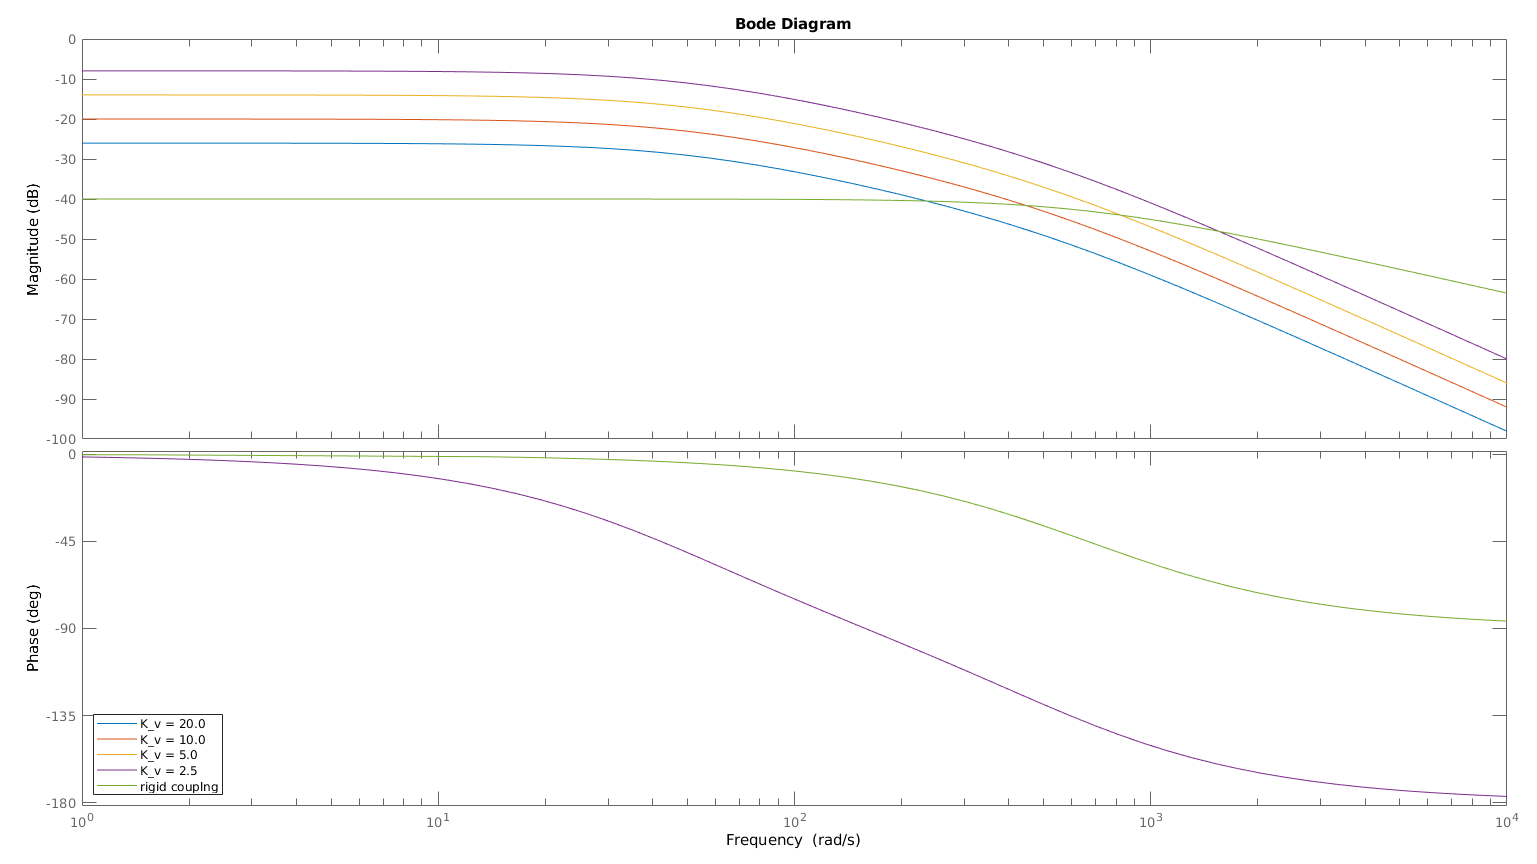
\includegraphics[width=0.9\linewidth]{Images/bodo}
	\caption{Bode diagram of the proposed vibration filter}
	\label{fig:bodo}
\end{figure}
For this reason, in order to reach better task execution performances we want to
reduce the impact of invironment vibrations at minimum.\\
This could be accomplished, as shown before, by building an ad-hoc filter, such
as fig.\ref{fig:bodo} depicits, in which there are different slope profiles that
will end up rejecting the disturbances at higher frequencies than the cut-off ones and preserving the
signal at lower ones.\\
Analizying the two opposite behaviours: \textbf{rigid coupling} and \textbf{induced virtual
compliance} which is achieved through the choice of the desired cut-off
frequencies ( which converted in Htz are respectively equal to 8 and 80 Htz ),
it is intresting the comparation of the vibration suppression applied on three different noise frequencies ( $10^{1}$,$10^{2}$and $10^{2} Htz$):
\begin{itemize}
\item In fig.\ref{fig:10Htz} is shown how the vibrations at lower frequencies are preserved by the
\textsl{virtual compliance},this is a rather desiderable aspect of a teleoperation interaction
since the input commands generated by the controller will have kind of low frequencies.
\item The fig.\ref{fig:100Htz} demonstrates a turning point in which the
disturbance rejection achieved by the \textsl{rigid coupling} is comparable to
the performance of the Set 1 of \textsl{virtual compliance} parameters.
\item At frequencies higher than the cut-off ones, the
vibrations will be dumped more effectly by the sets of computed virtual
parameters than with \textsl{rigid coupling}, this is deducible from fig.\ref{fig:1000Htz}.
\end{itemize}

\begin{figure}
	\begin{subfigure}[h!]{1\linewidth}
		\centering
		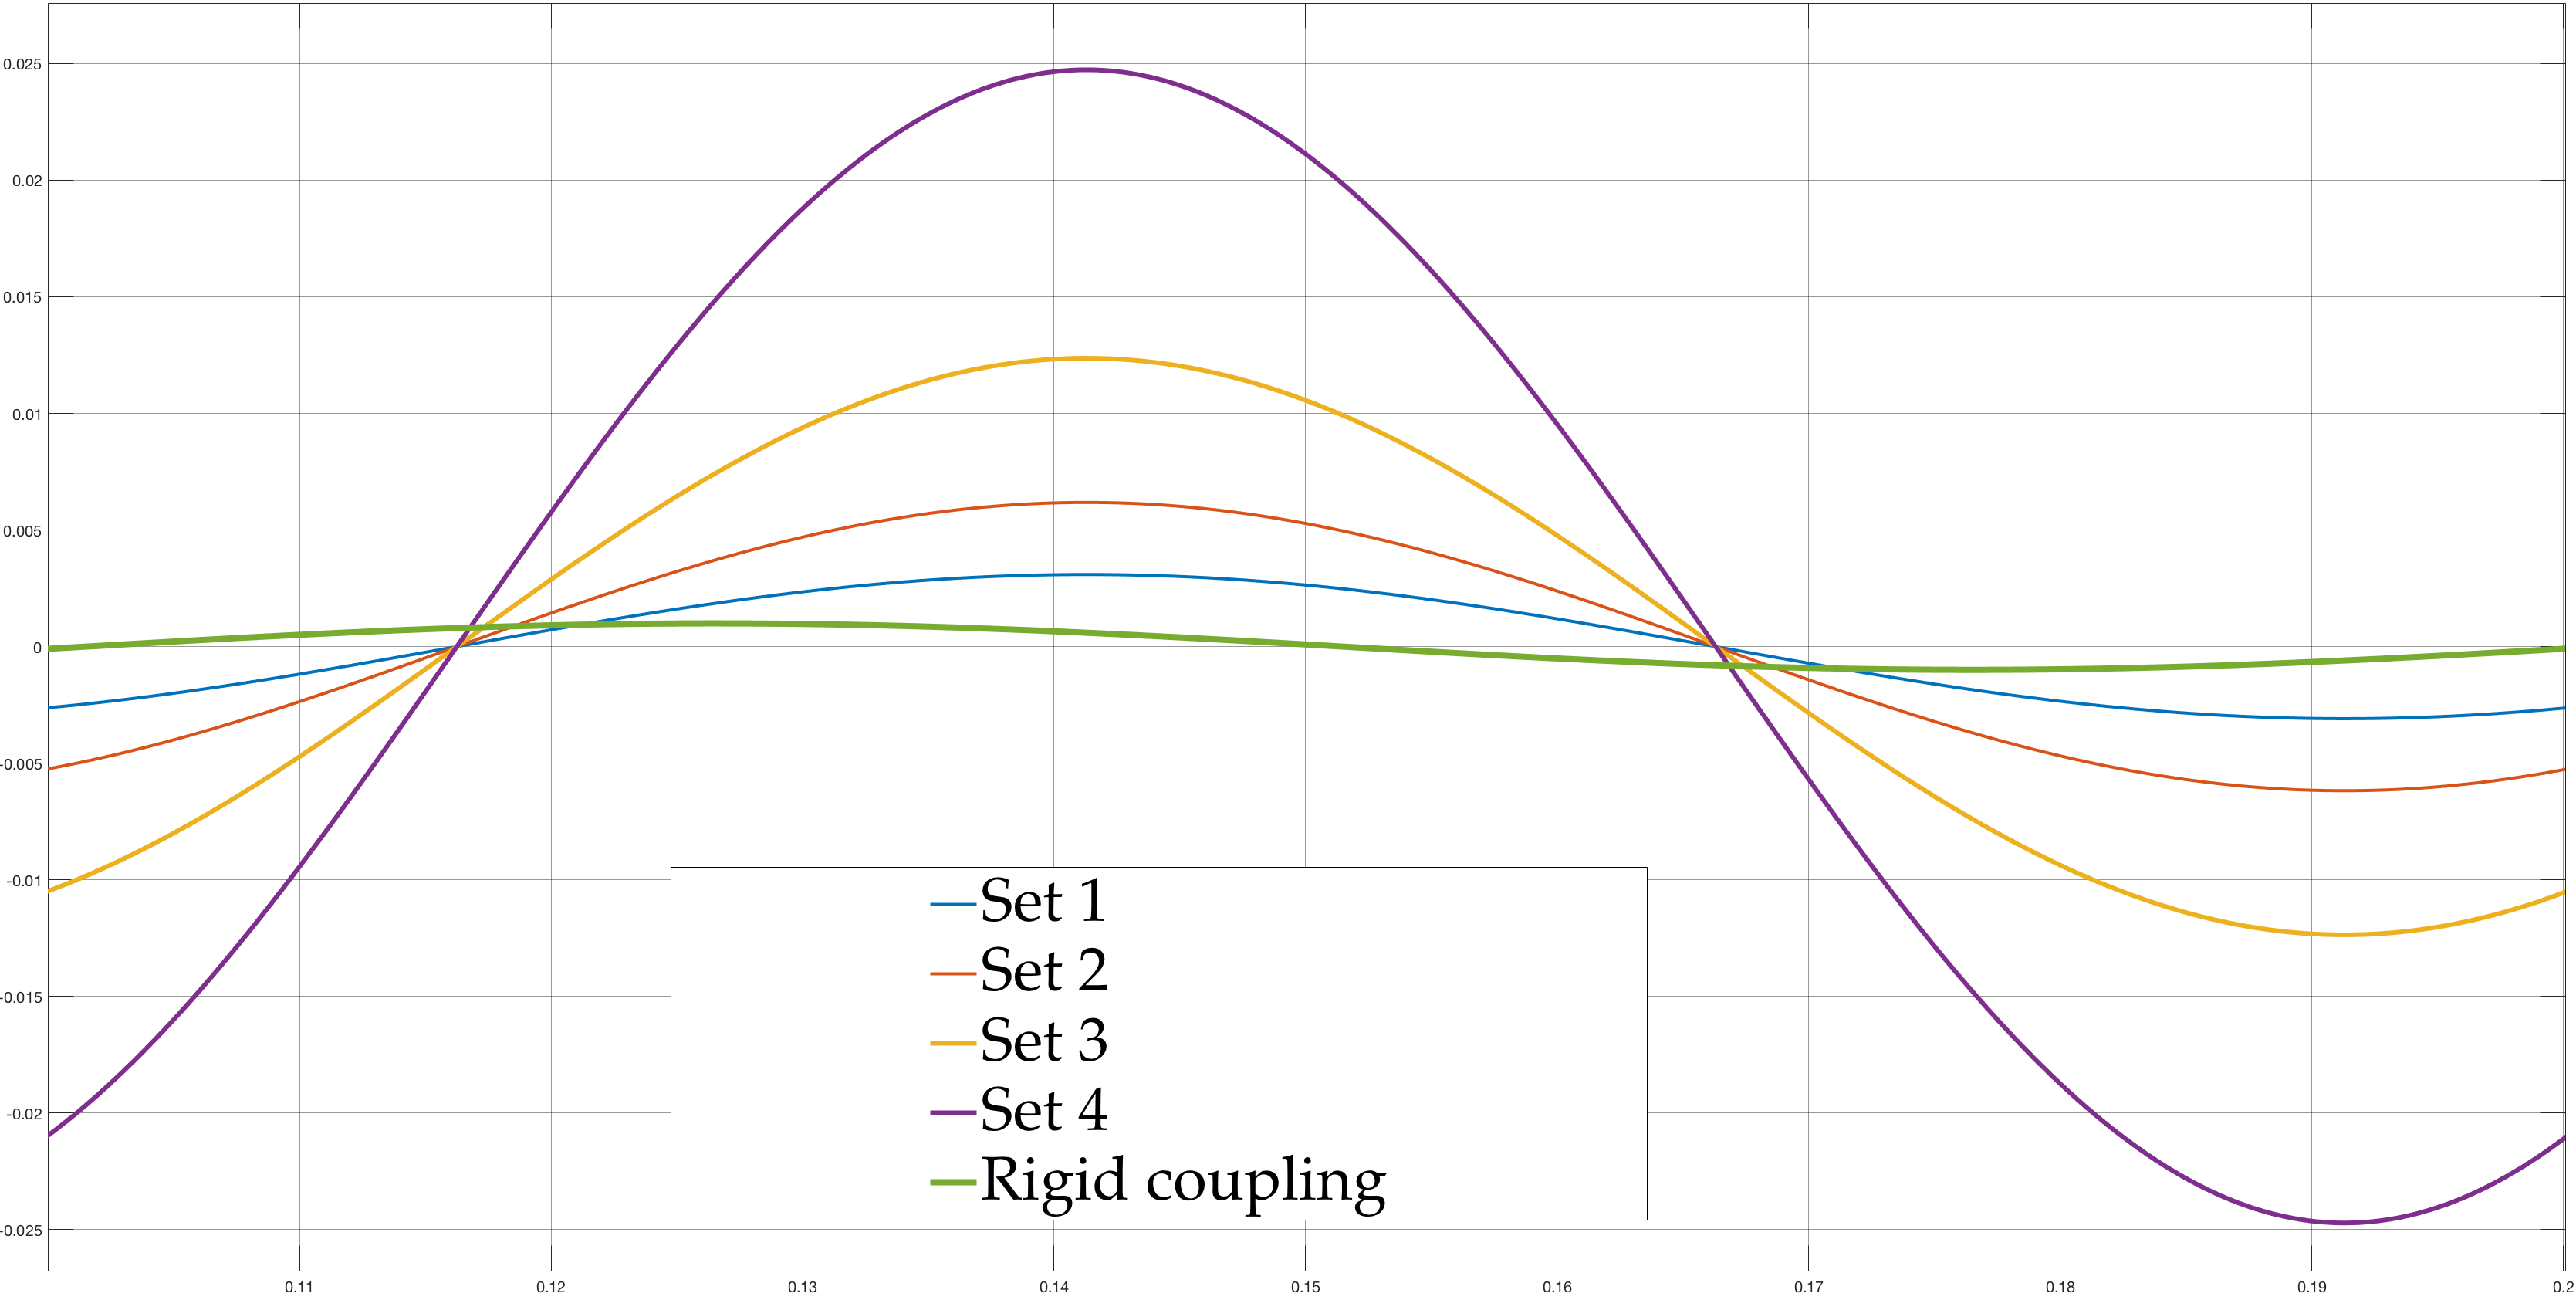
\includegraphics[width=\textwidth, height=\textwidth/3]{Images/vibr10Htz}
		\caption{10 Htz}
		\label{fig:10Htz}
	\end{subfigure}	
  \newline
	\begin{subfigure}[h!]{1\linewidth}
		\centering
		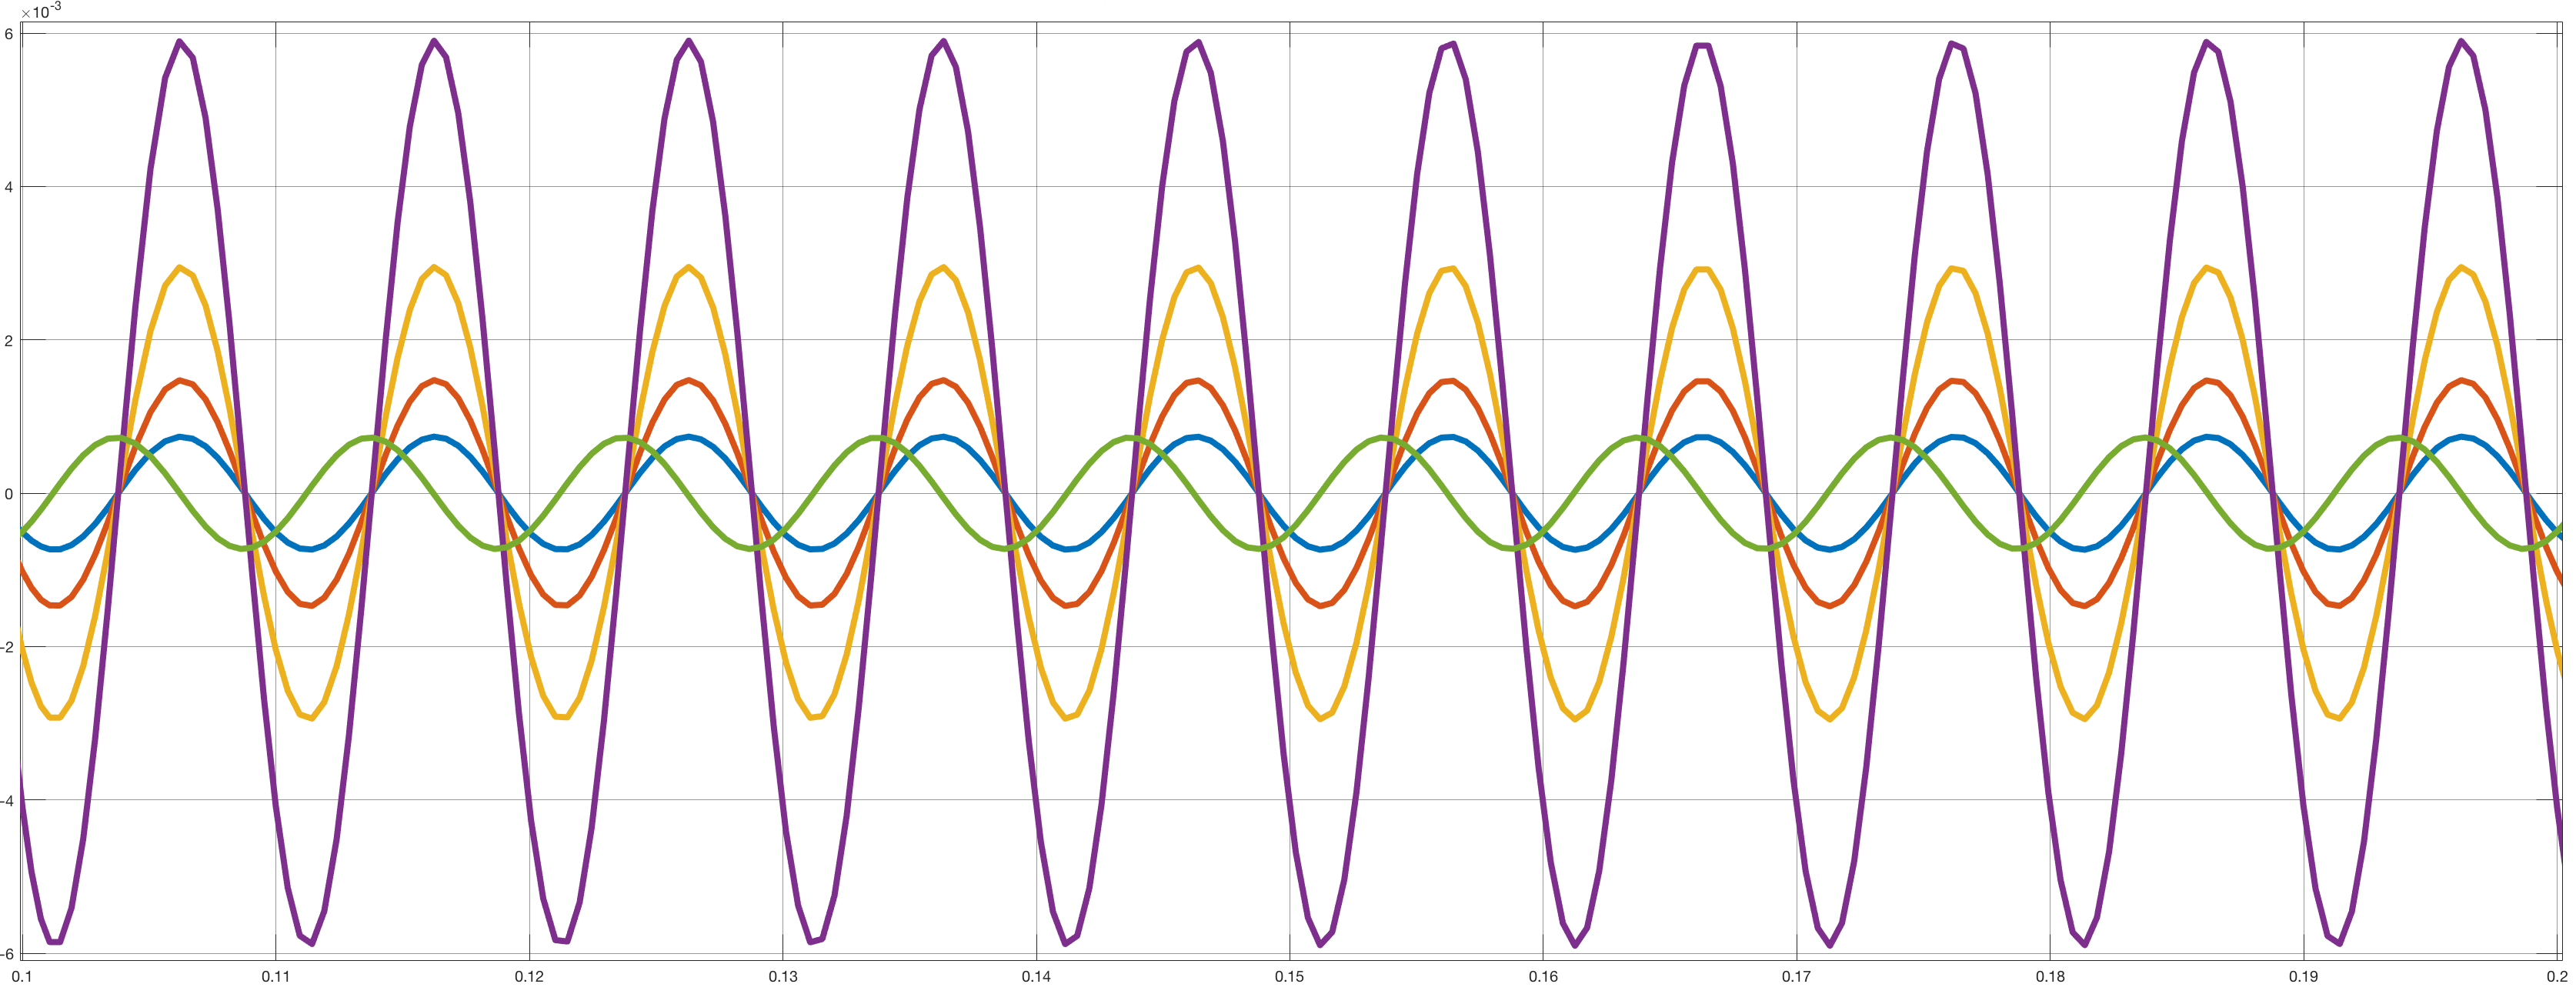
\includegraphics[width=\textwidth, height=\textwidth/3]{Images/vibr100Htz}
		\caption{100 Htz}
		\label{fig:100Htz}
	\end{subfigure}	
  \newline
	\begin{subfigure}[h!]{1\linewidth}
		\centering.
		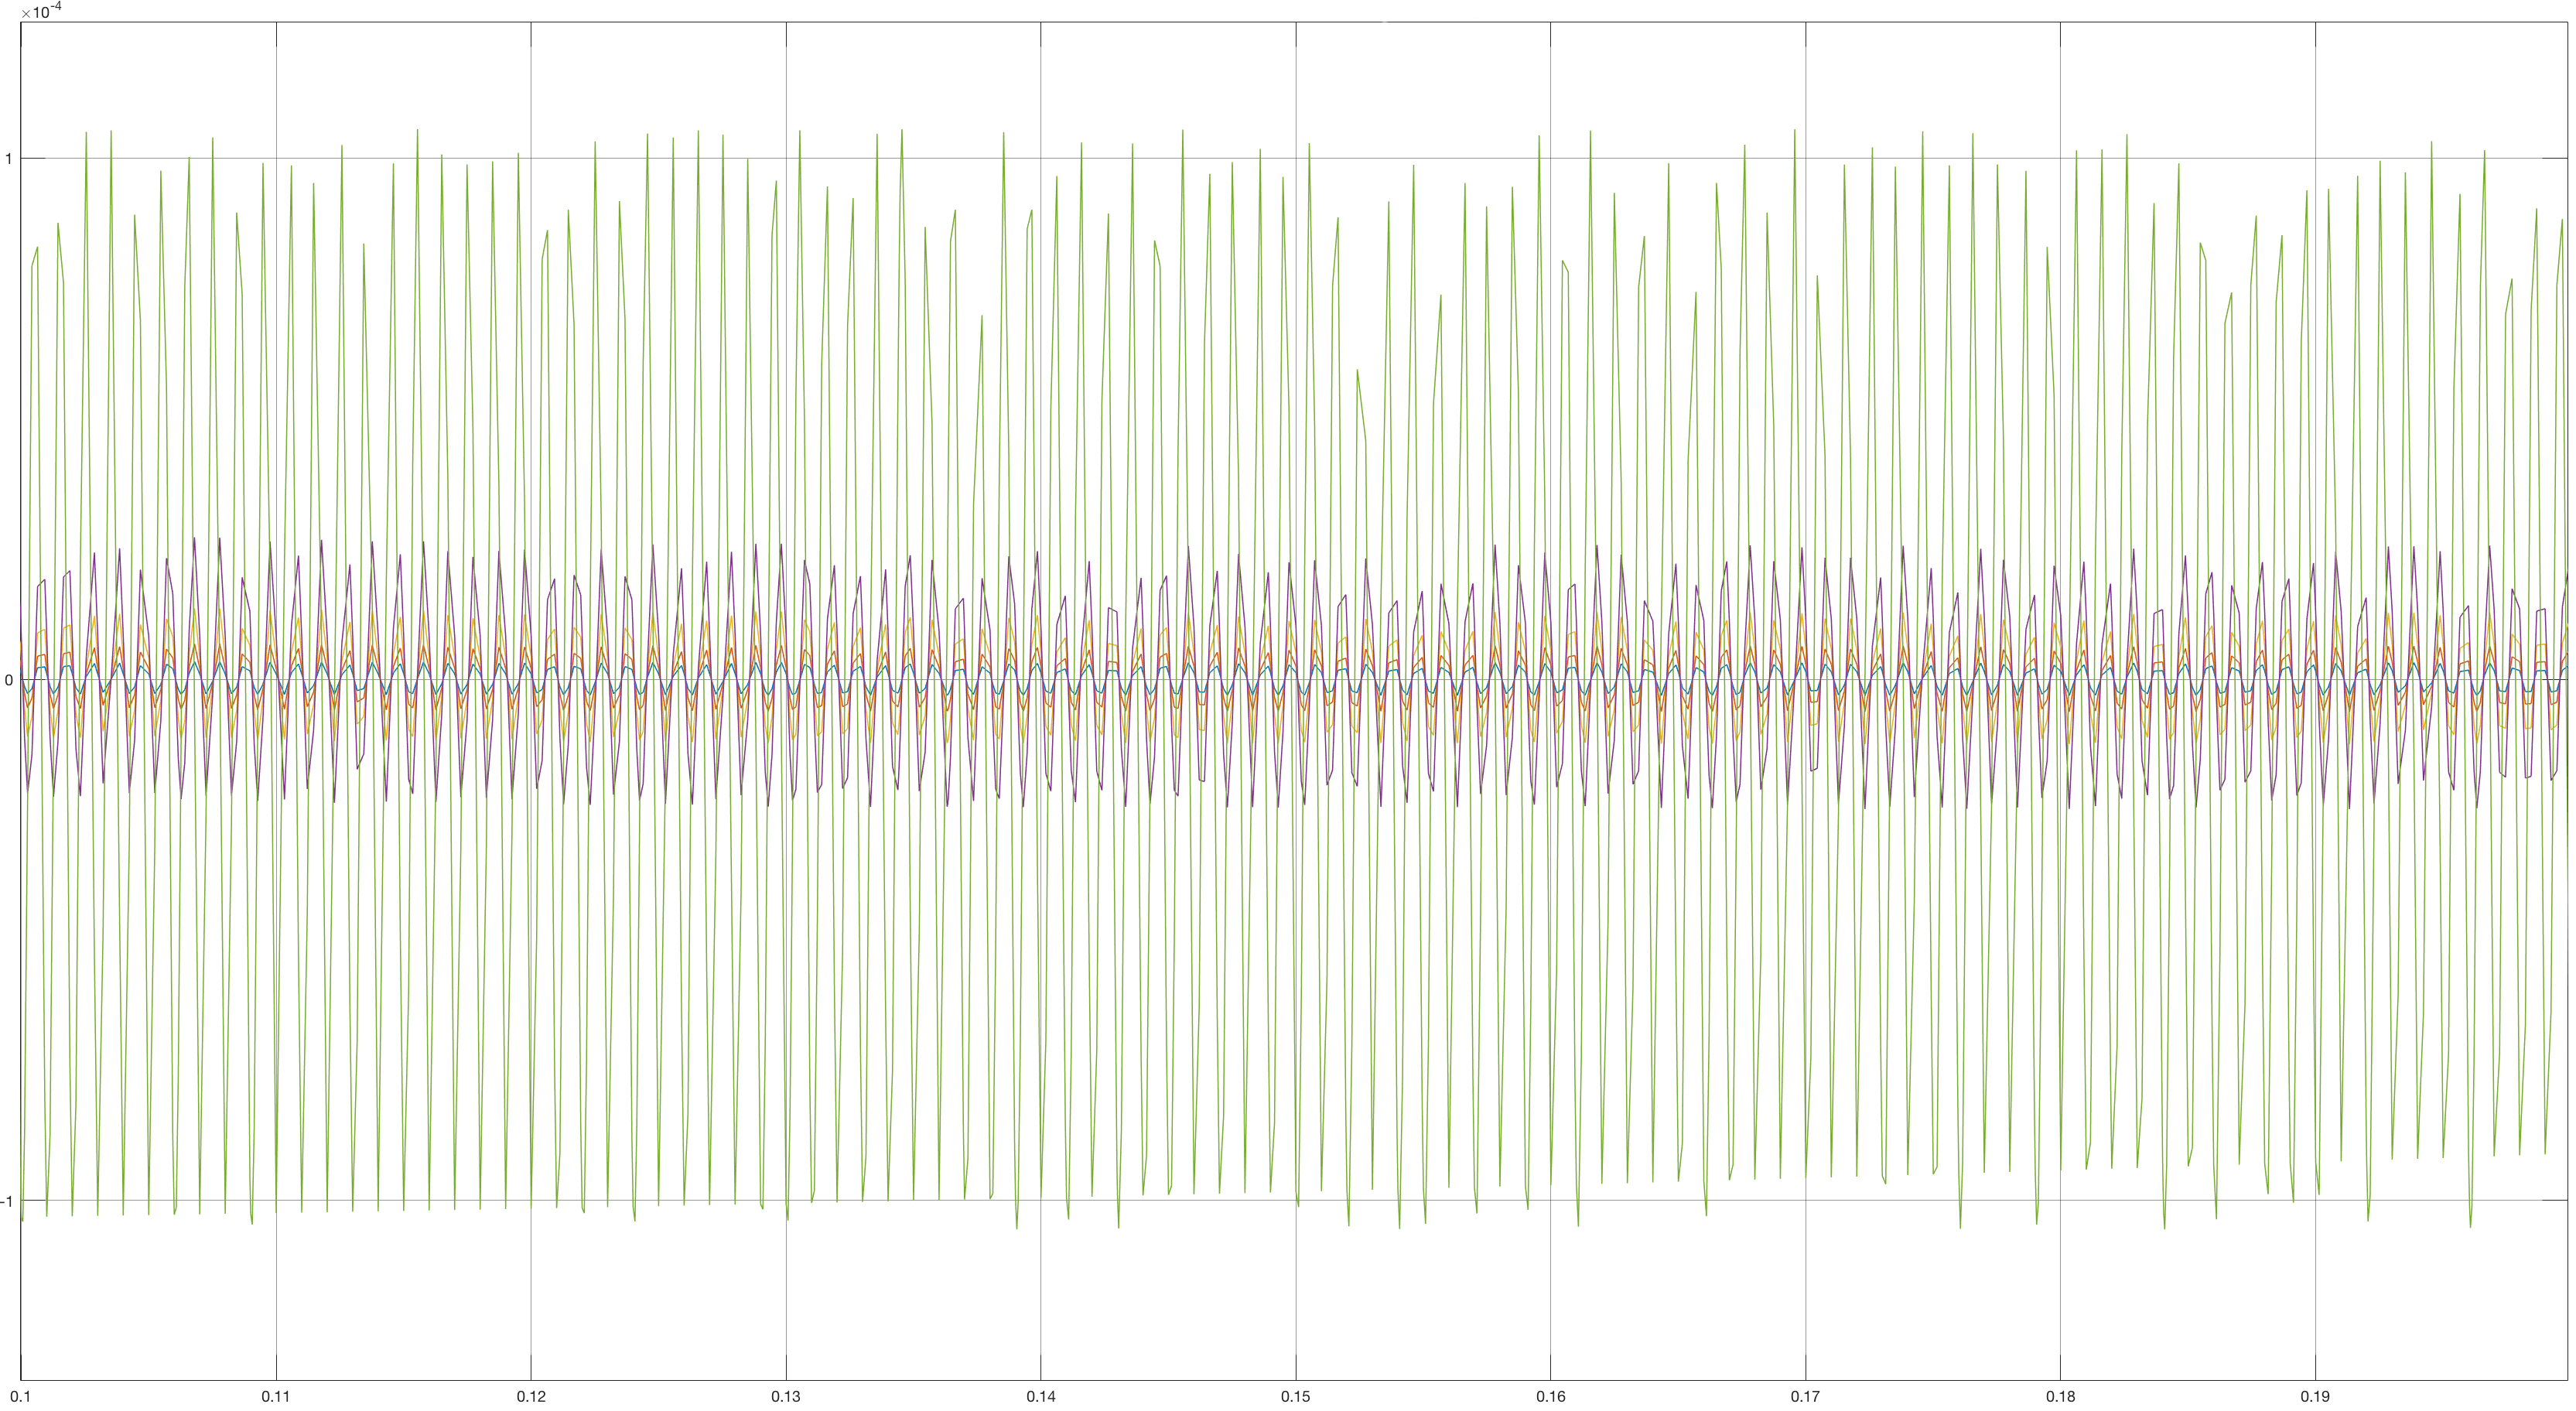
\includegraphics[width=\textwidth, height=\textwidth/3]{Images/vibr1000Htz}
		\caption{1000 Htz}
		\label{fig:1000Htz}
	\end{subfigure}
\caption{ Signal response to a noise with three different frequencies modulated 
  by the proposed vibration damping filter.}
\end{figure}

\newpage

\subsection{Task execution analisys}

\subsubsection{Free motion with high noise frequencies}

At first, we present an execution in free motion where , the
slave succeds to follow the trajectory given to the master, applying both
\textsl{rigid coupling} (fig.\ref{fig:freeRigTot50HR}) and \textsl{virtual
  compliance} (fig.\ref{fig:freeSetTot50HR}), with almost no task error
(without considering the error due to noise disturbances).
This kind of disturbance should be damped, and in fact, using \textsl{virtual
  compliance} (fig.\ref{fig:freeRigPar50HR}) the profile of the angle is smoother
than in \textsl{rigid coupling} (fig.\ref{fig:freeSetPar50HR}).

\begin{figure}
	\begin{subfigure}[h!]{1\linewidth}
		\centering
		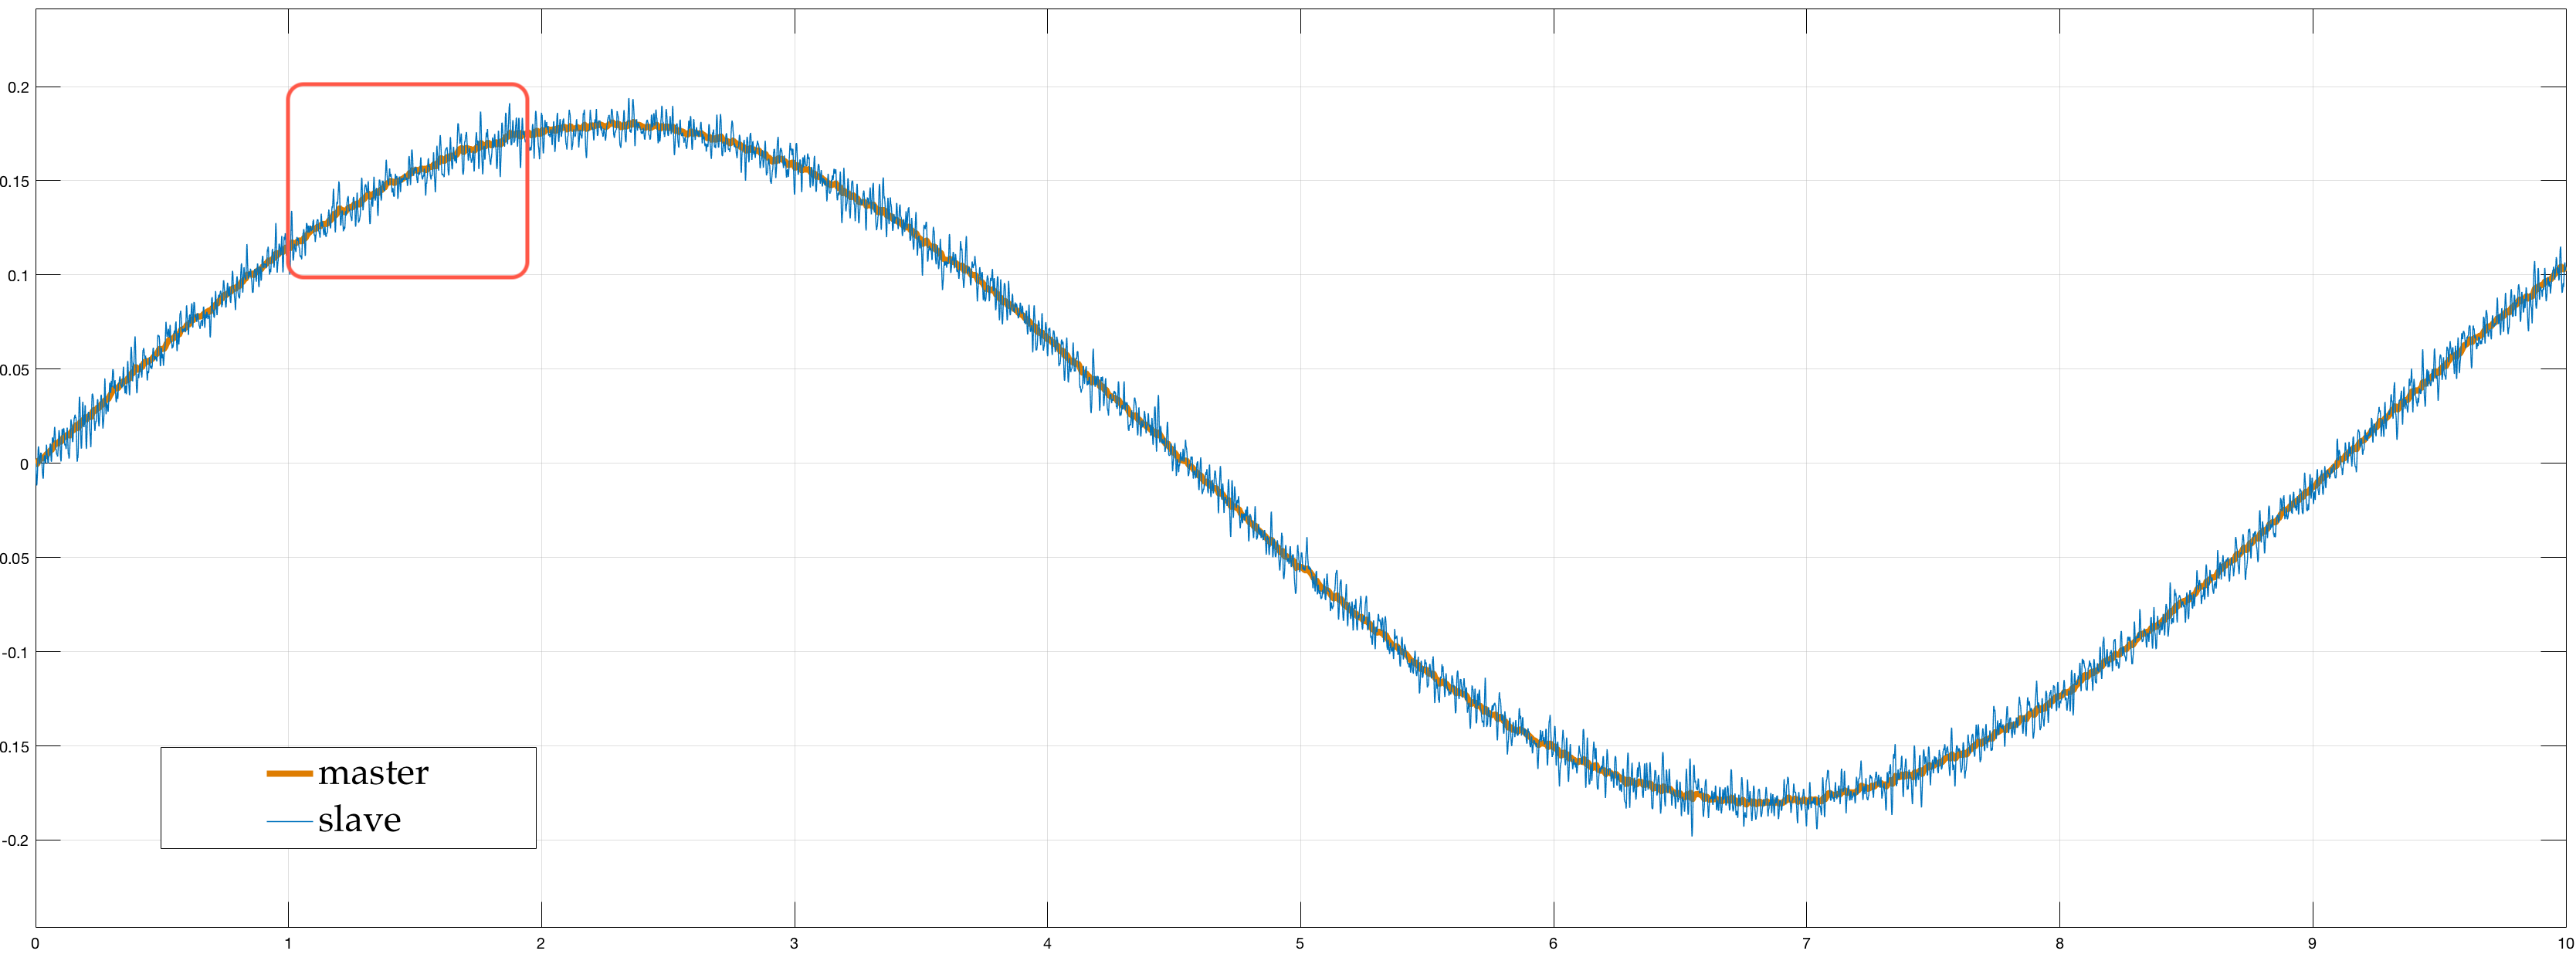
\includegraphics[width=\textwidth, height=\textwidth/4]{Images/rCoupFreeTot50htznoiseRect}
		\caption{Rigid coupling}
		\label{fig:freeRigTot50HR}
	\end{subfigure}	
  \newline
	\begin{subfigure}[h!]{1\linewidth}
		\centering
		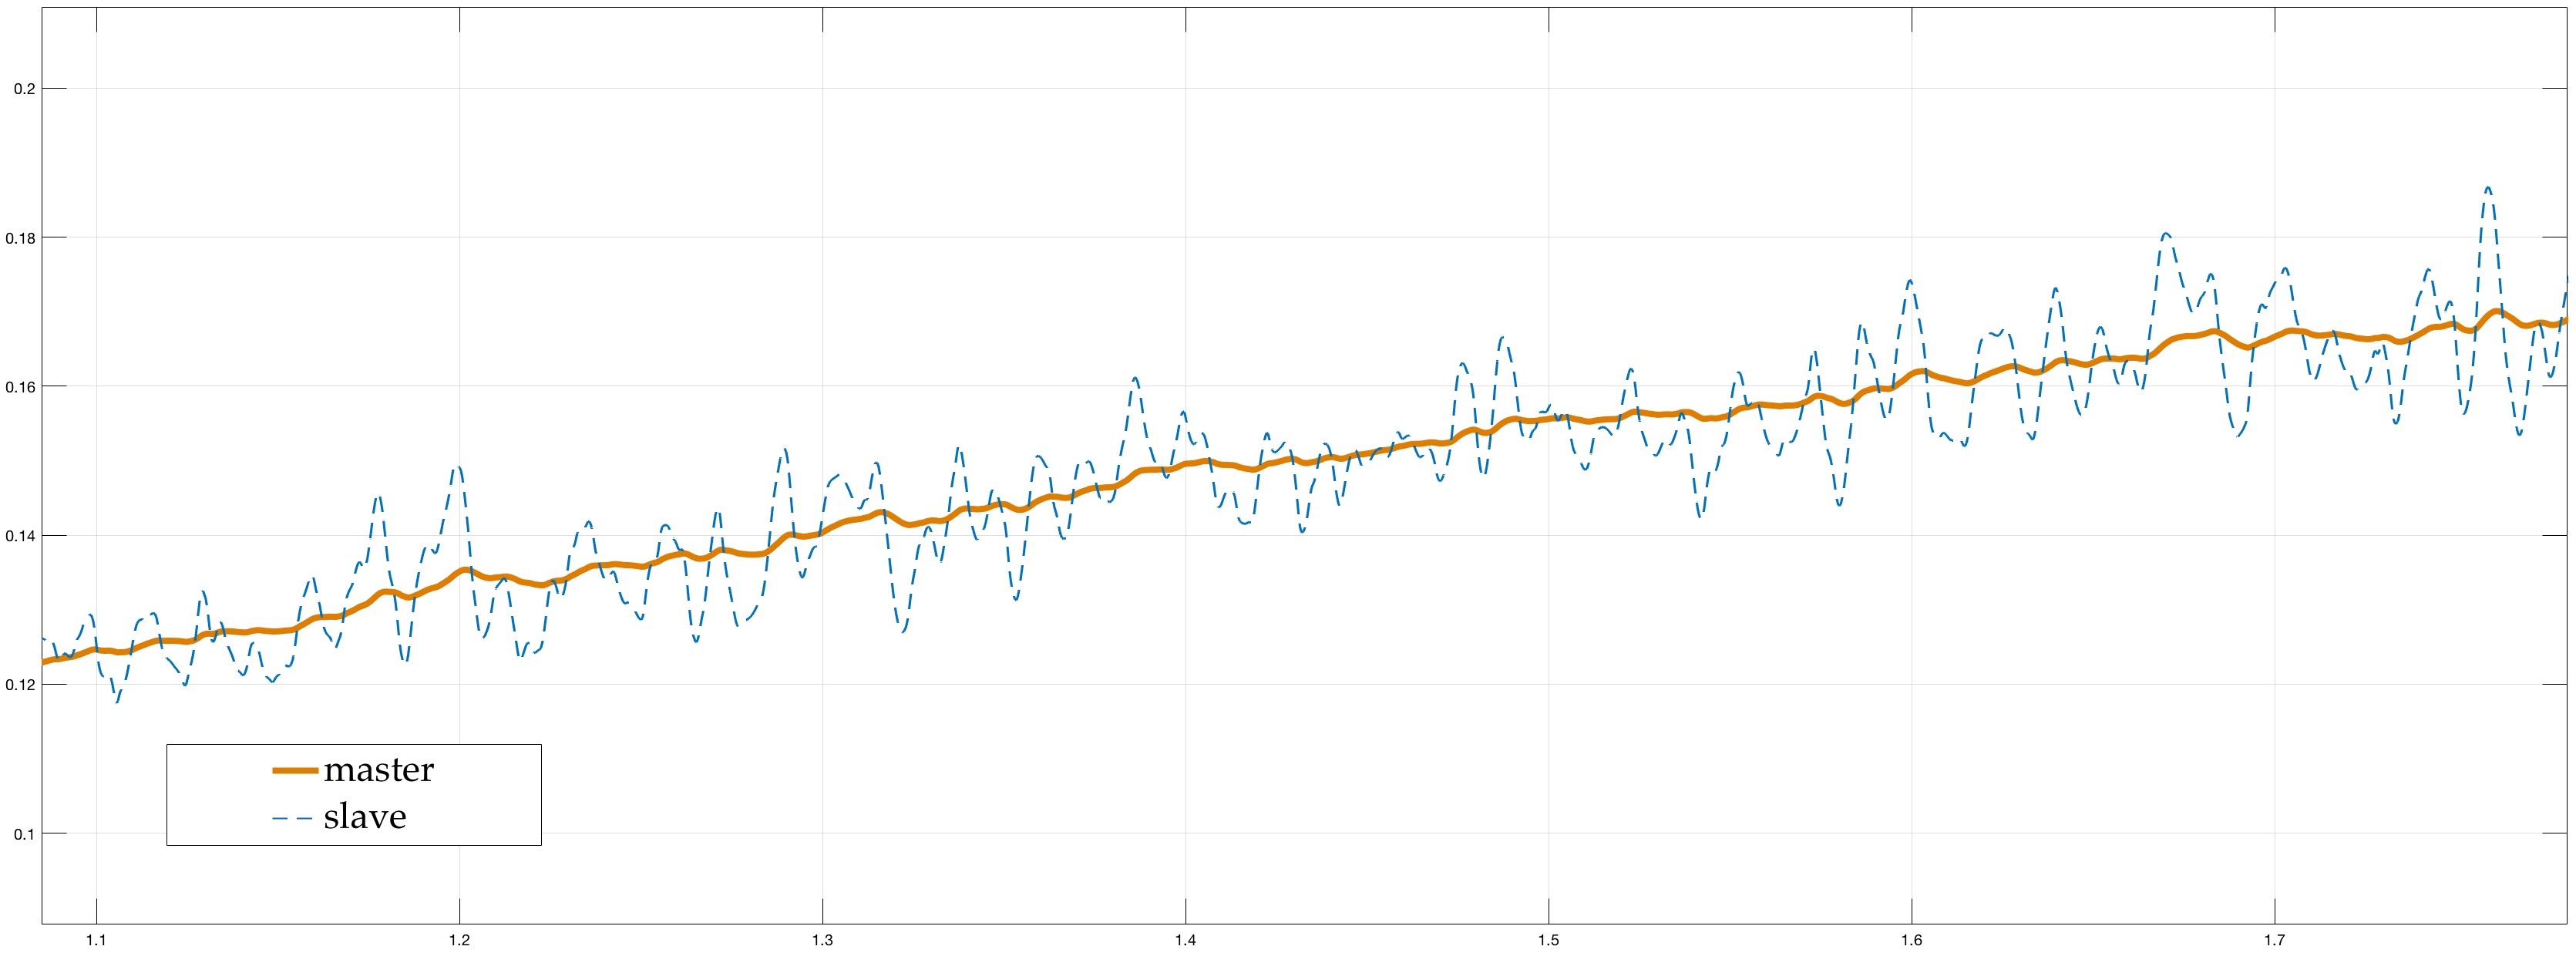
\includegraphics[width=\textwidth, height=\textwidth/4]{Images/rCoupFree50htznoise}
		\caption{Particular taken from the highlighted area in fig.\ref{fig:freeRigTot50HR}}
		\label{fig:freeRigPar50HR}
	\end{subfigure}	
  \newline
	\begin{subfigure}[h!]{1\linewidth}
		\centering
		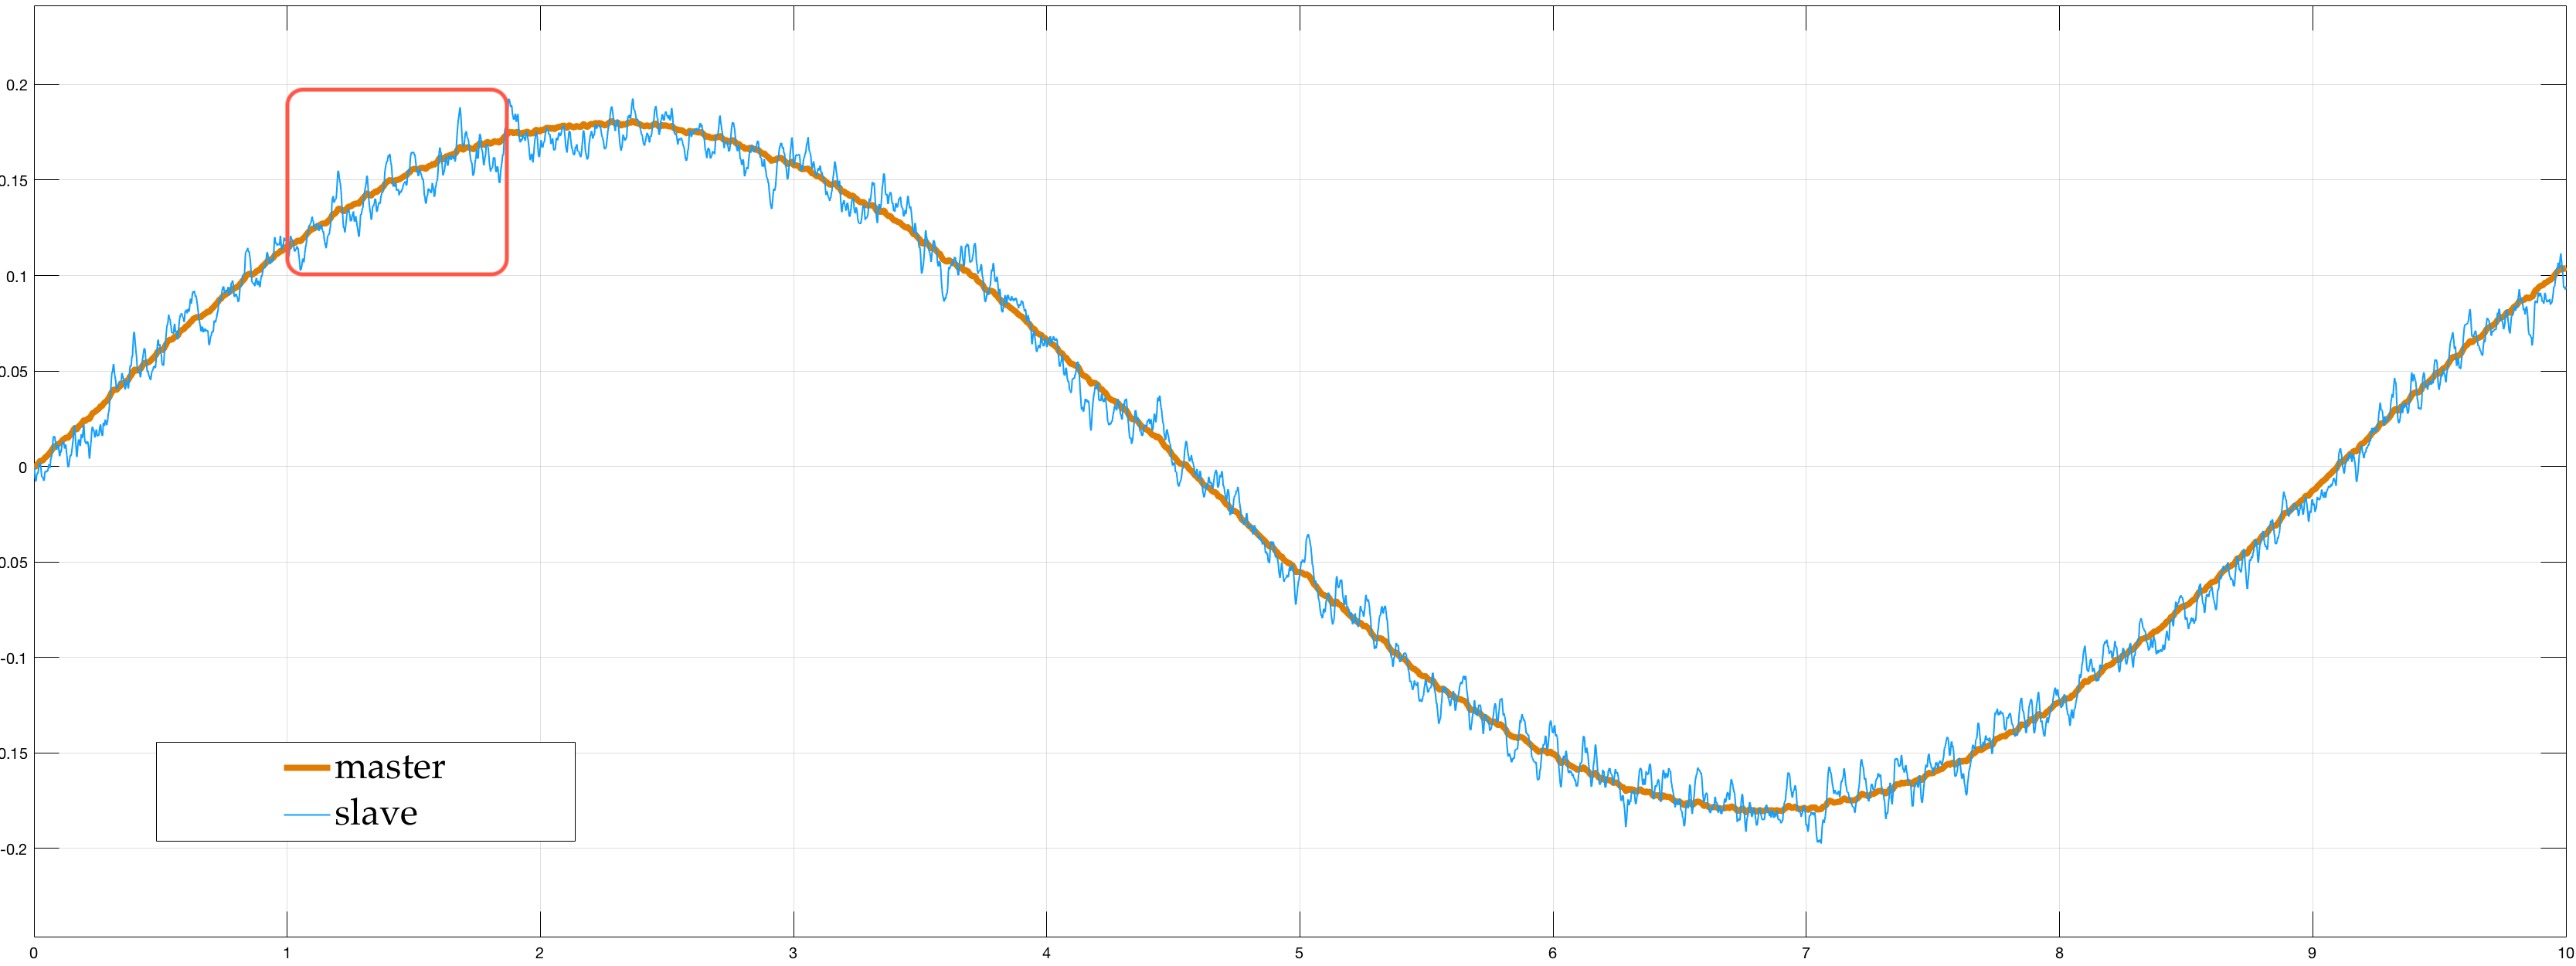
\includegraphics[width=\textwidth, height=\textwidth/4]{Images/set20freeTot50HtznoiseRect}
		\caption{Virtual compliance Set n.4}
		\label{fig:freeSetTot50HR}
	\end{subfigure}	
  \newline
	\begin{subfigure}[h!]{1\linewidth}
		\centering
		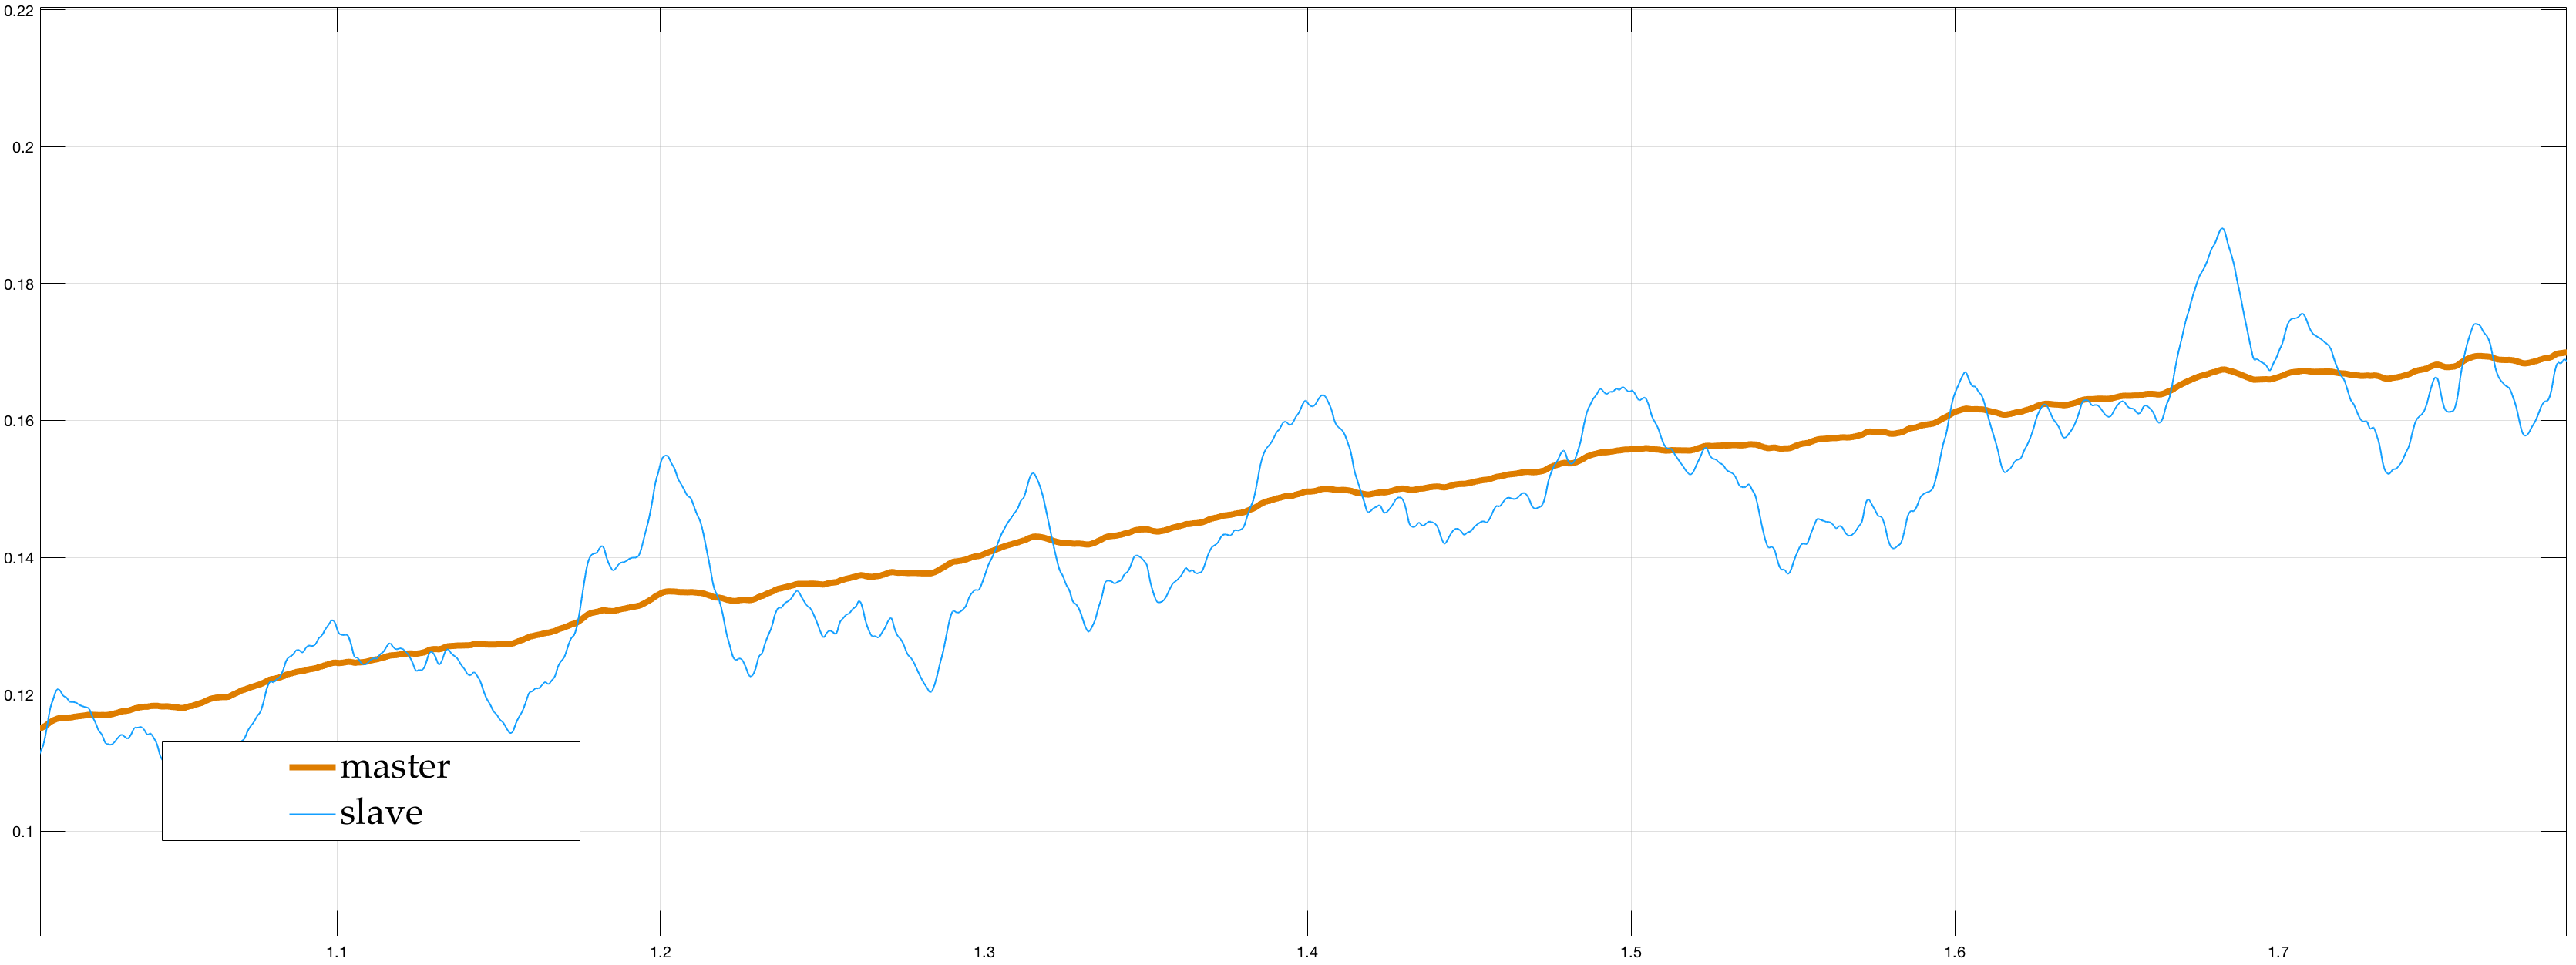
\includegraphics[width=\textwidth, height=\textwidth/4]{Images/set20freePart50Htznoise}
		\caption{Particular taken from the highlighted area in fig.\ref{fig:freeSetTot50HR}}
		\label{fig:freeSetPar50HR}
	\end{subfigure}	
  \caption{ Free motion master-slave simulation, with artificial disturbances at
    50 Htz frequency. }
\end{figure}






\subsubsection{Free motion with low noise frequencies}

Comparatively, two other simulations have been undertaken that share the same
conditions of the previous ones, if not for the noise frequence, which has been lowered.
This kind of disturbance is usually a similar to the input of the control
actuators, so it should be preserved, namely it shouldn't be affected by the
proposed filtering.\\
This phenomenon shows up in fig.\ref{fig:freeRigPar20HR} and fig.\ref{fig:freeSetPar20HR}.
In fact, if compared, the two profiles confirm that \textsl{rigid coupling}
cancel out most of the healty signal, on the contrary \textsl{virtual
  compliance} save the signal information, which is extremely important from a
control perspective.

\begin{figure}
	\begin{subfigure}[h!]{1\linewidth}
		\centering
		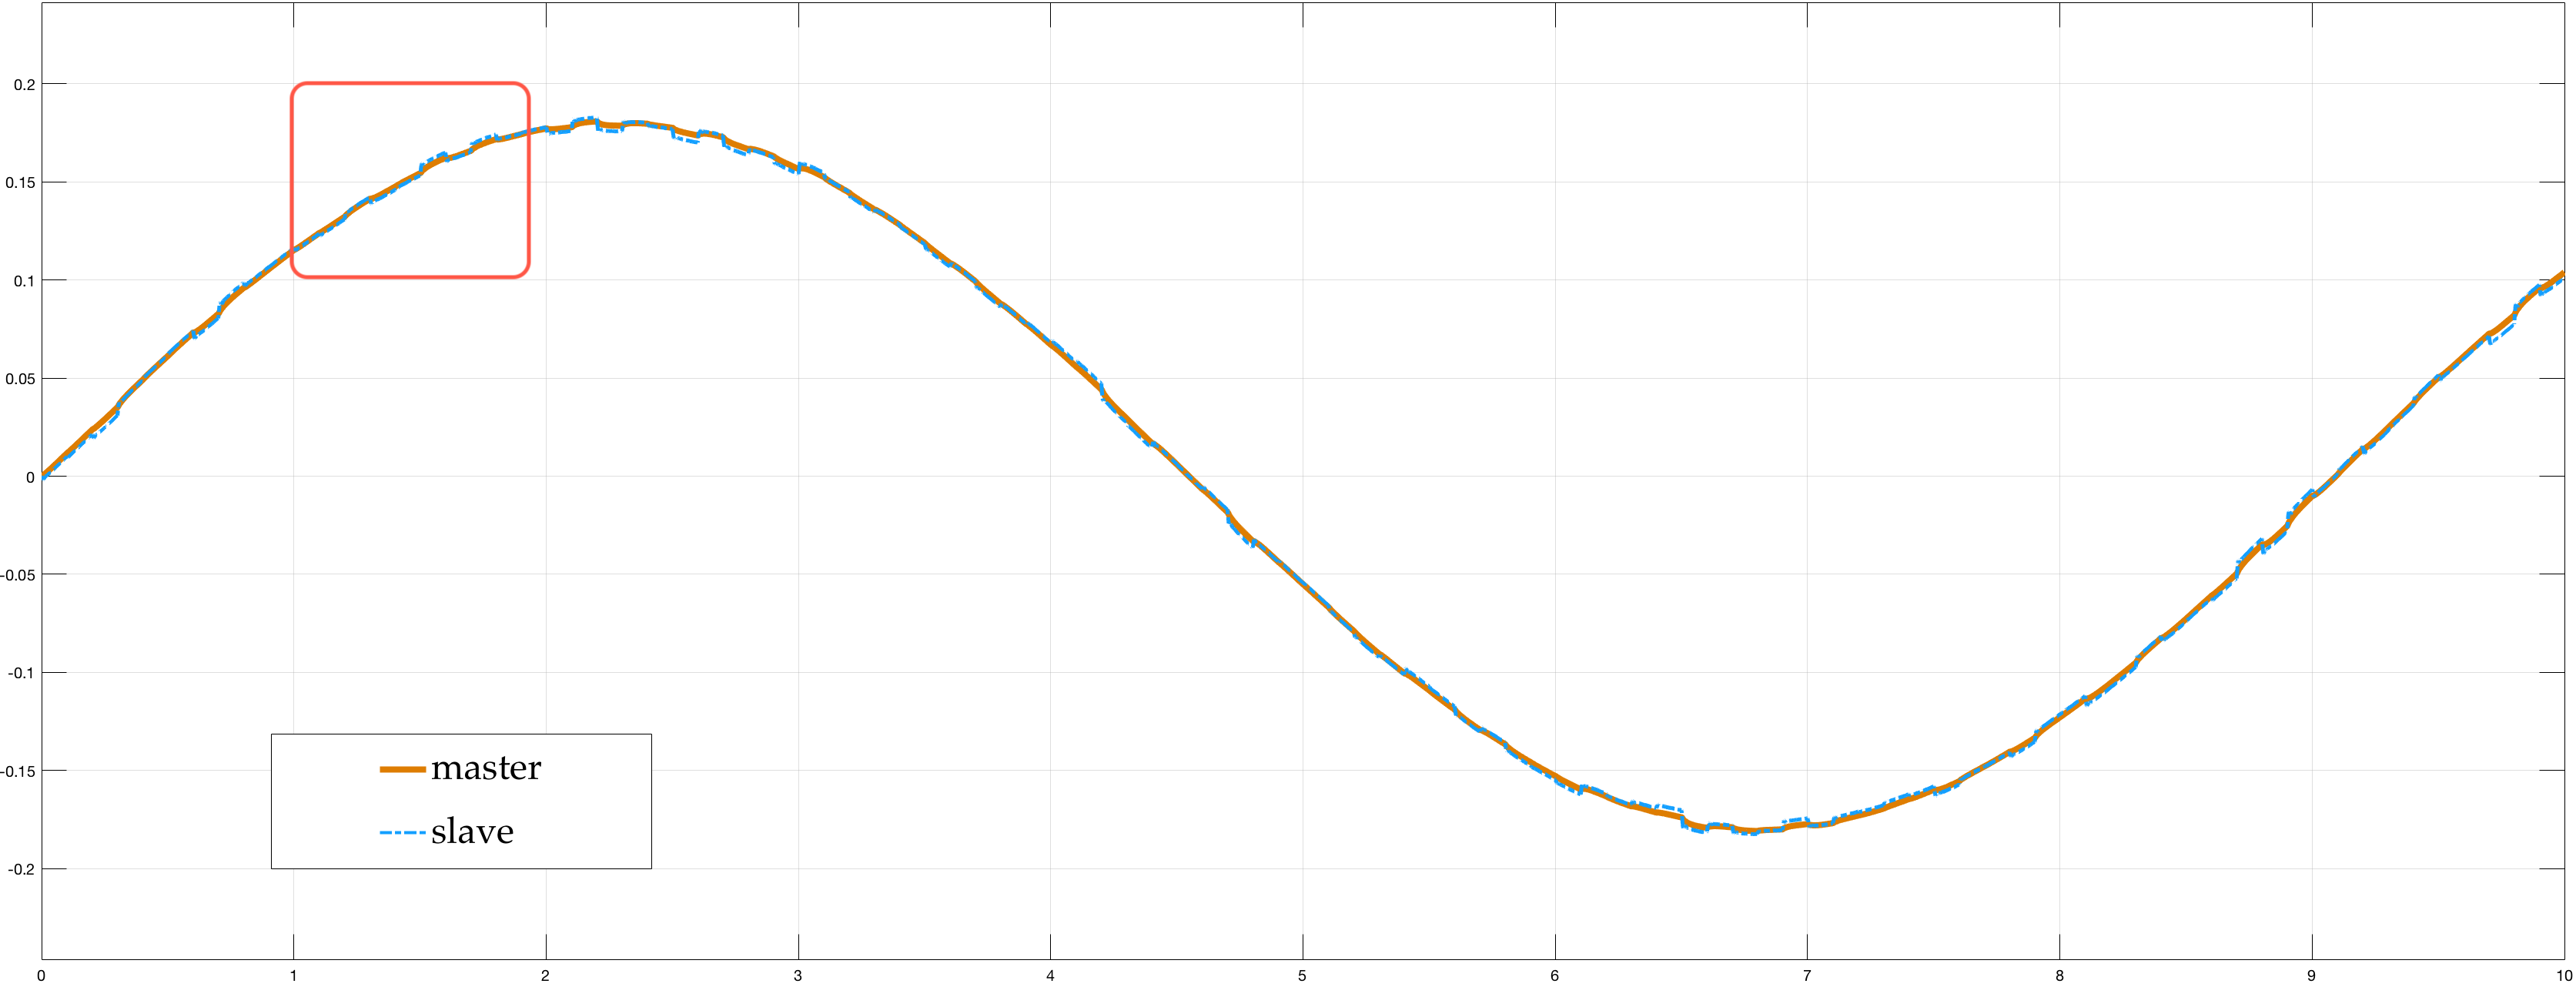
\includegraphics[width=\textwidth, height=\textwidth/4]{Images/freerigidTot20HtznoiseRect}
		\caption{ Rigid coupling }
		\label{fig:freeRigTot20HR}
	\end{subfigure}	
  \newline
	\begin{subfigure}[h!]{1\linewidth}
		\centering
		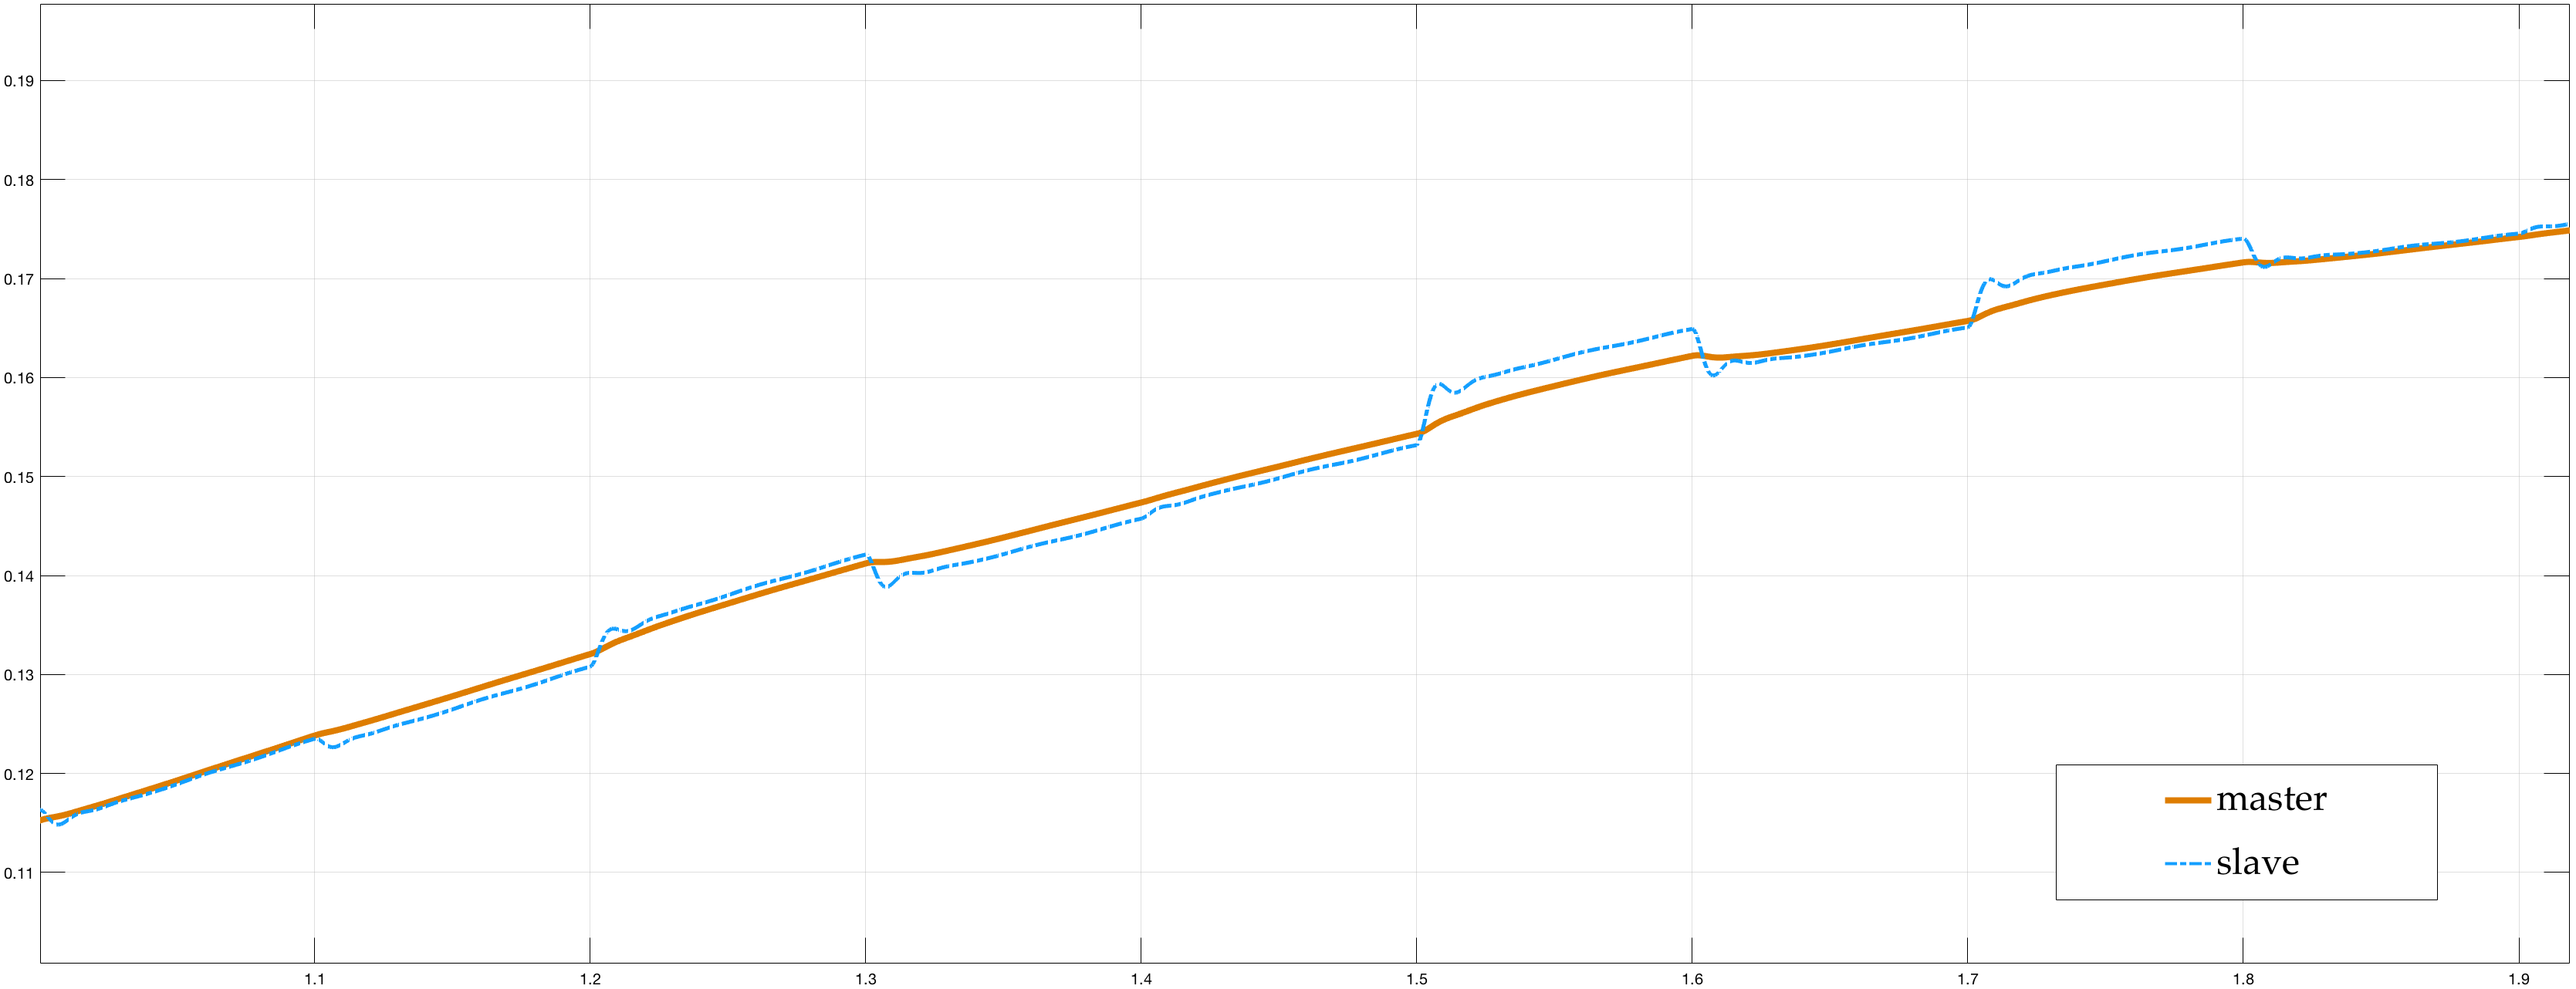
\includegraphics[width=\textwidth, height=\textwidth/4]{Images/freerigidPart20Htznoise}
		\caption{Particular taken from the highlighted area in fig.\ref{fig:freeRigTot20HR}}
		\label{fig:freeRigPar20HR}
	\end{subfigure}	
  \newline
	\begin{subfigure}[h!]{1\linewidth}
		\centering
		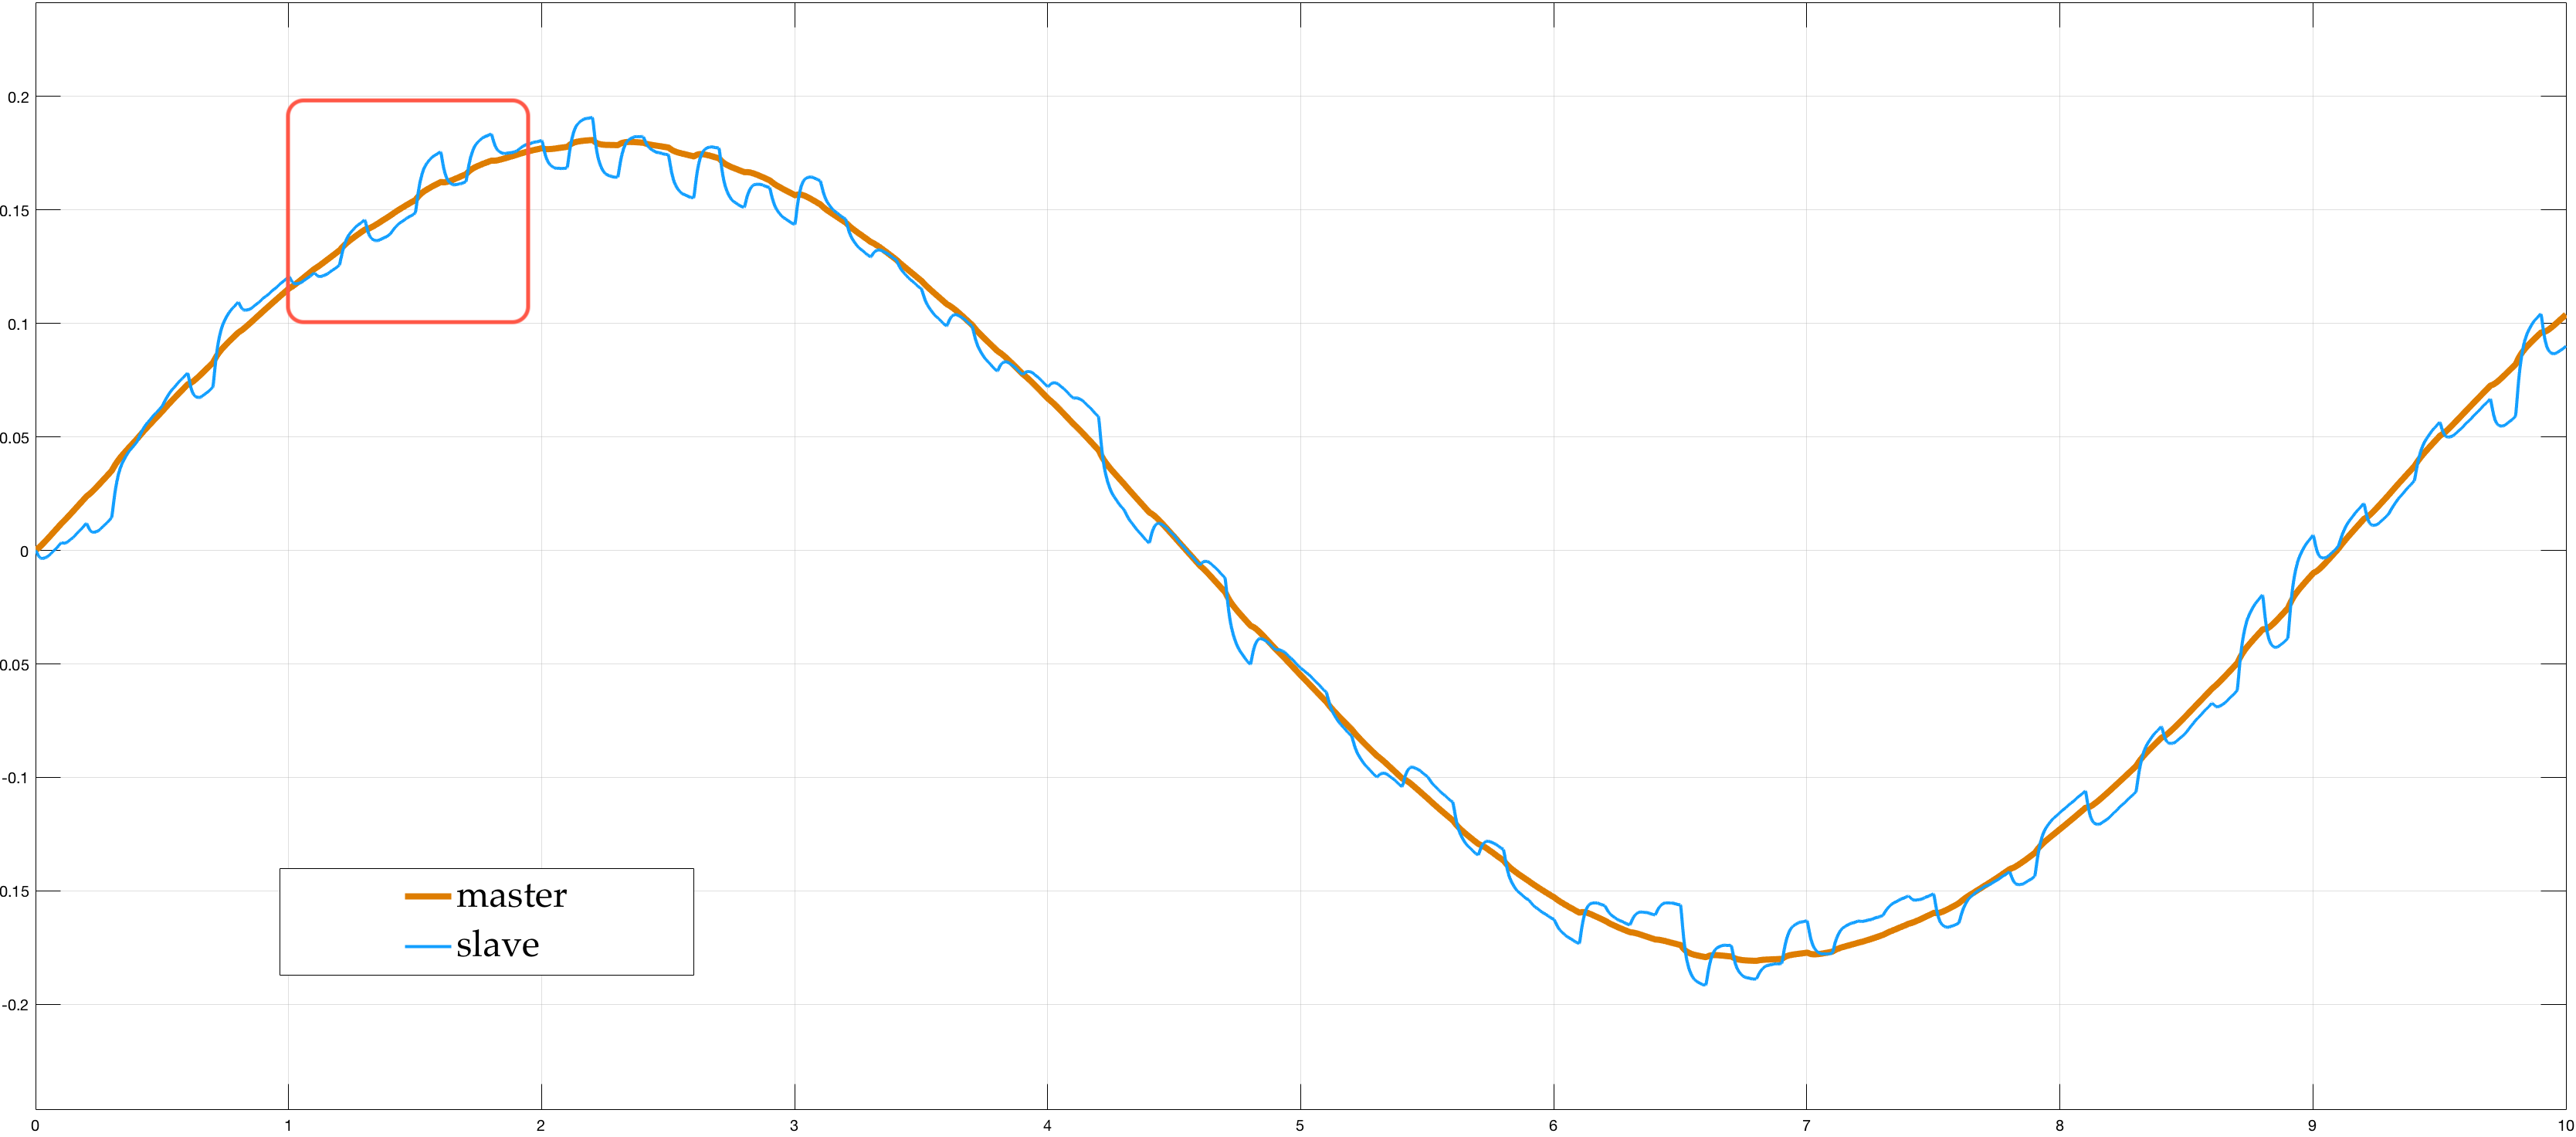
\includegraphics[width=\textwidth, height=\textwidth/4]{Images/freeSet20Tot20HtznoiseRect}
		\caption{Virtual compliance Set n.4}
		\label{fig:freeSetTot20HR}
	\end{subfigure}	
  \newline
	\begin{subfigure}[h!]{1\linewidth}
		\centering
		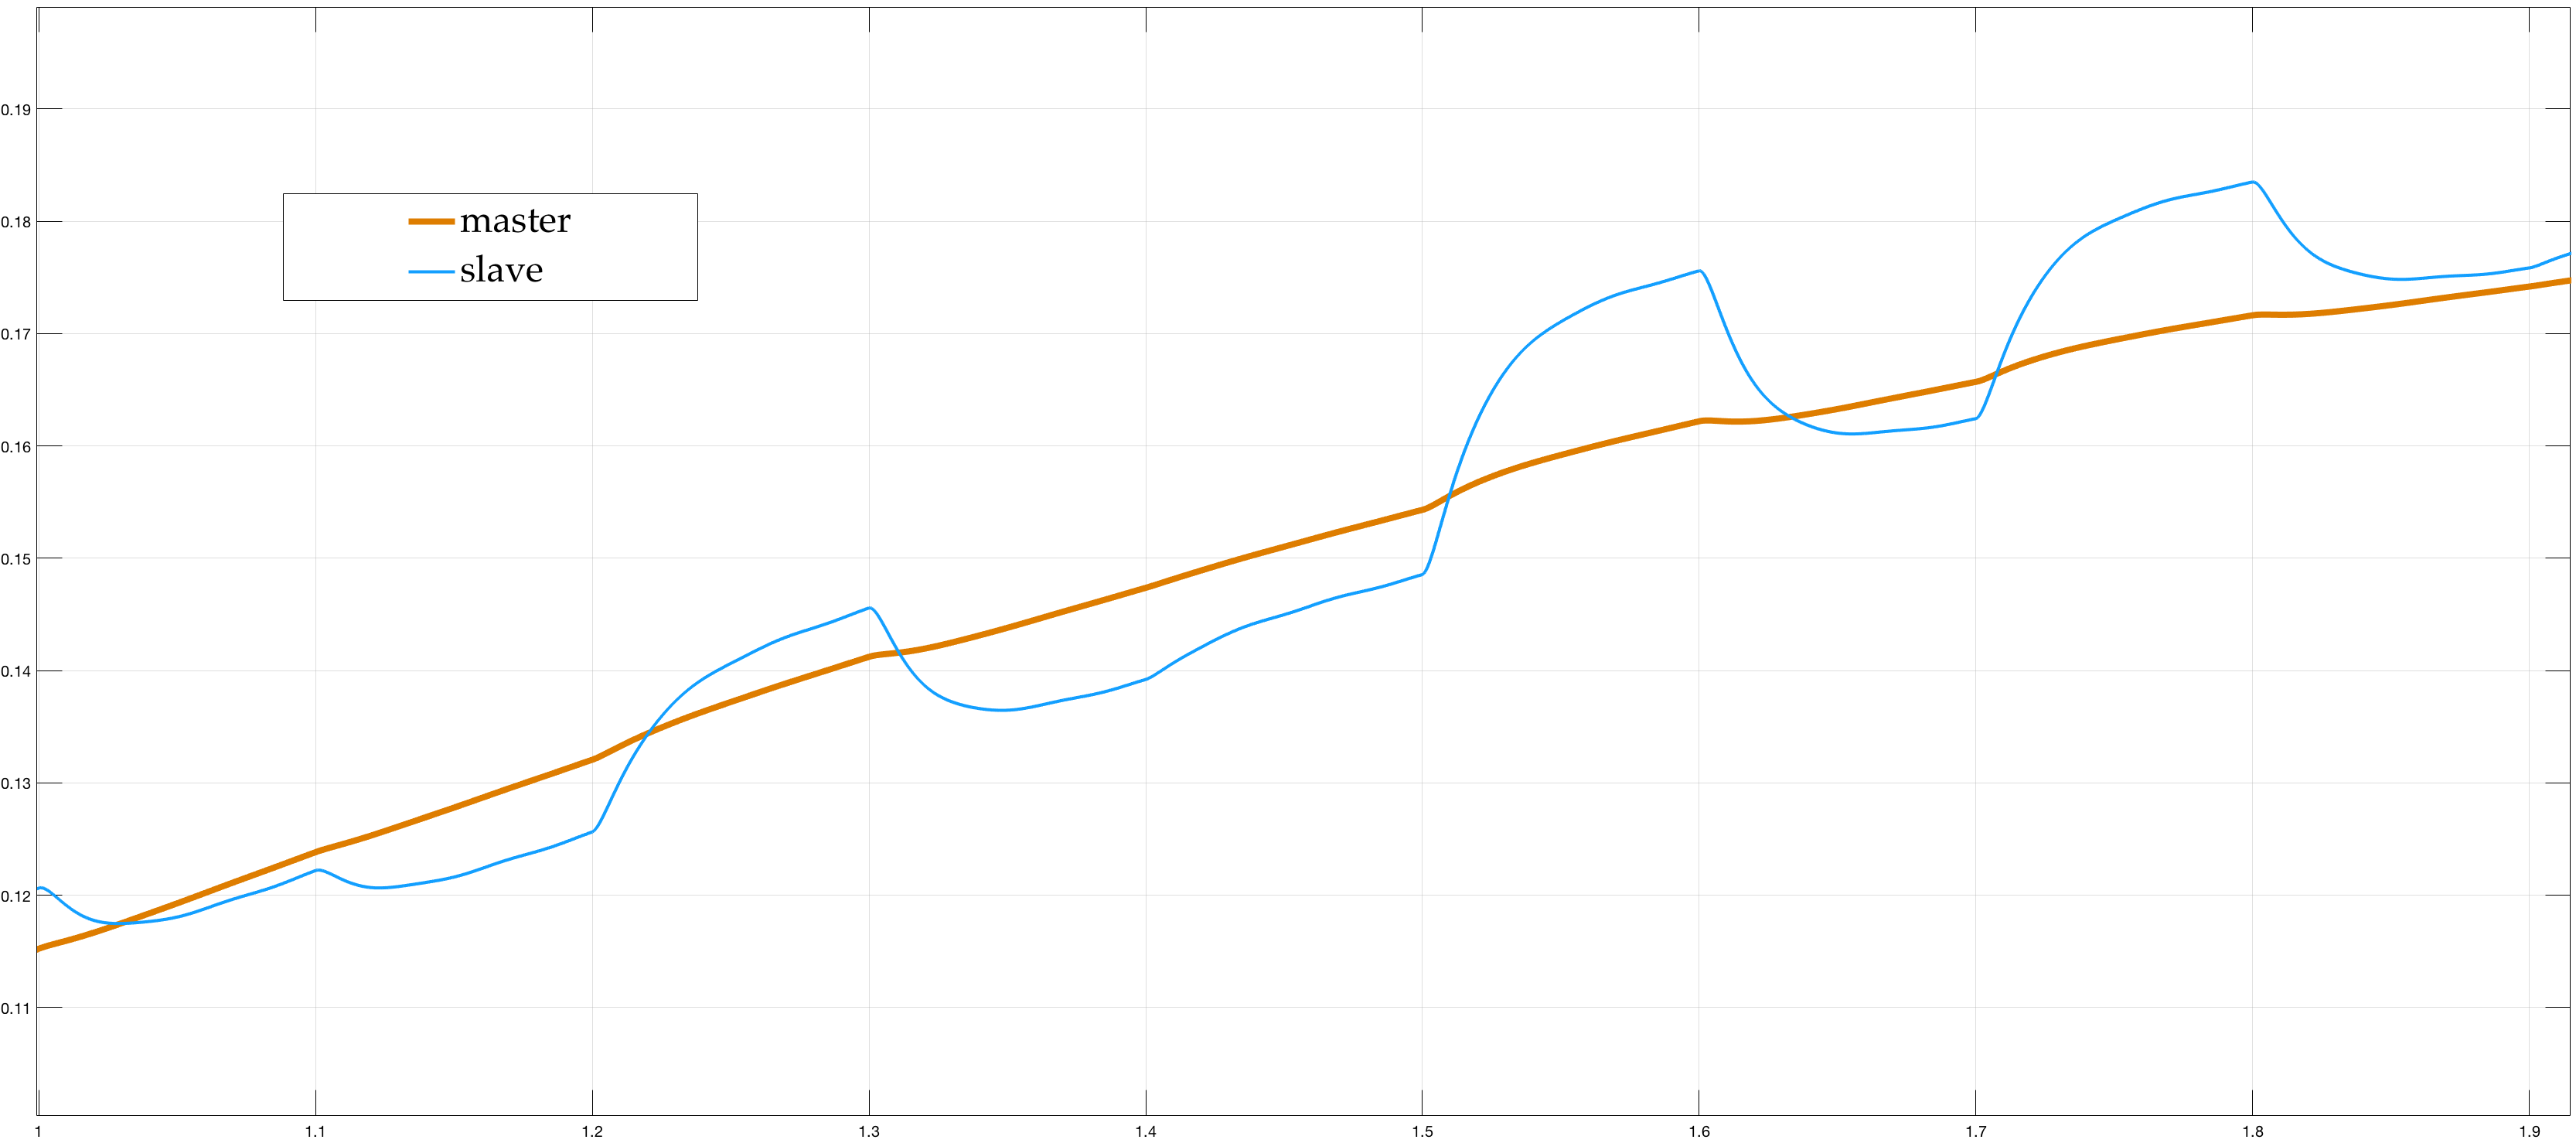
\includegraphics[width=\textwidth, height=\textwidth/4]{Images/freeSet20Part20Htznoise}
		\caption{Particular taken from the highlighted area in fig.\ref{fig:freeSetTot20HR}}
		\label{fig:freeSetPar20HR}
	\end{subfigure}	
  \caption{ Free motion master-slave simulation, with artificial disturbances at
    20 Htz frequency.}
\end{figure}


\subsubsection{Environment contact }

Here the proposed simulations hold the same reference trajectory for master.
But, in addiction, after that the slave would trespass a certaing angle value
there would be a contact with the environment.



% \begin{figure}[h]
% 	\centering
% 	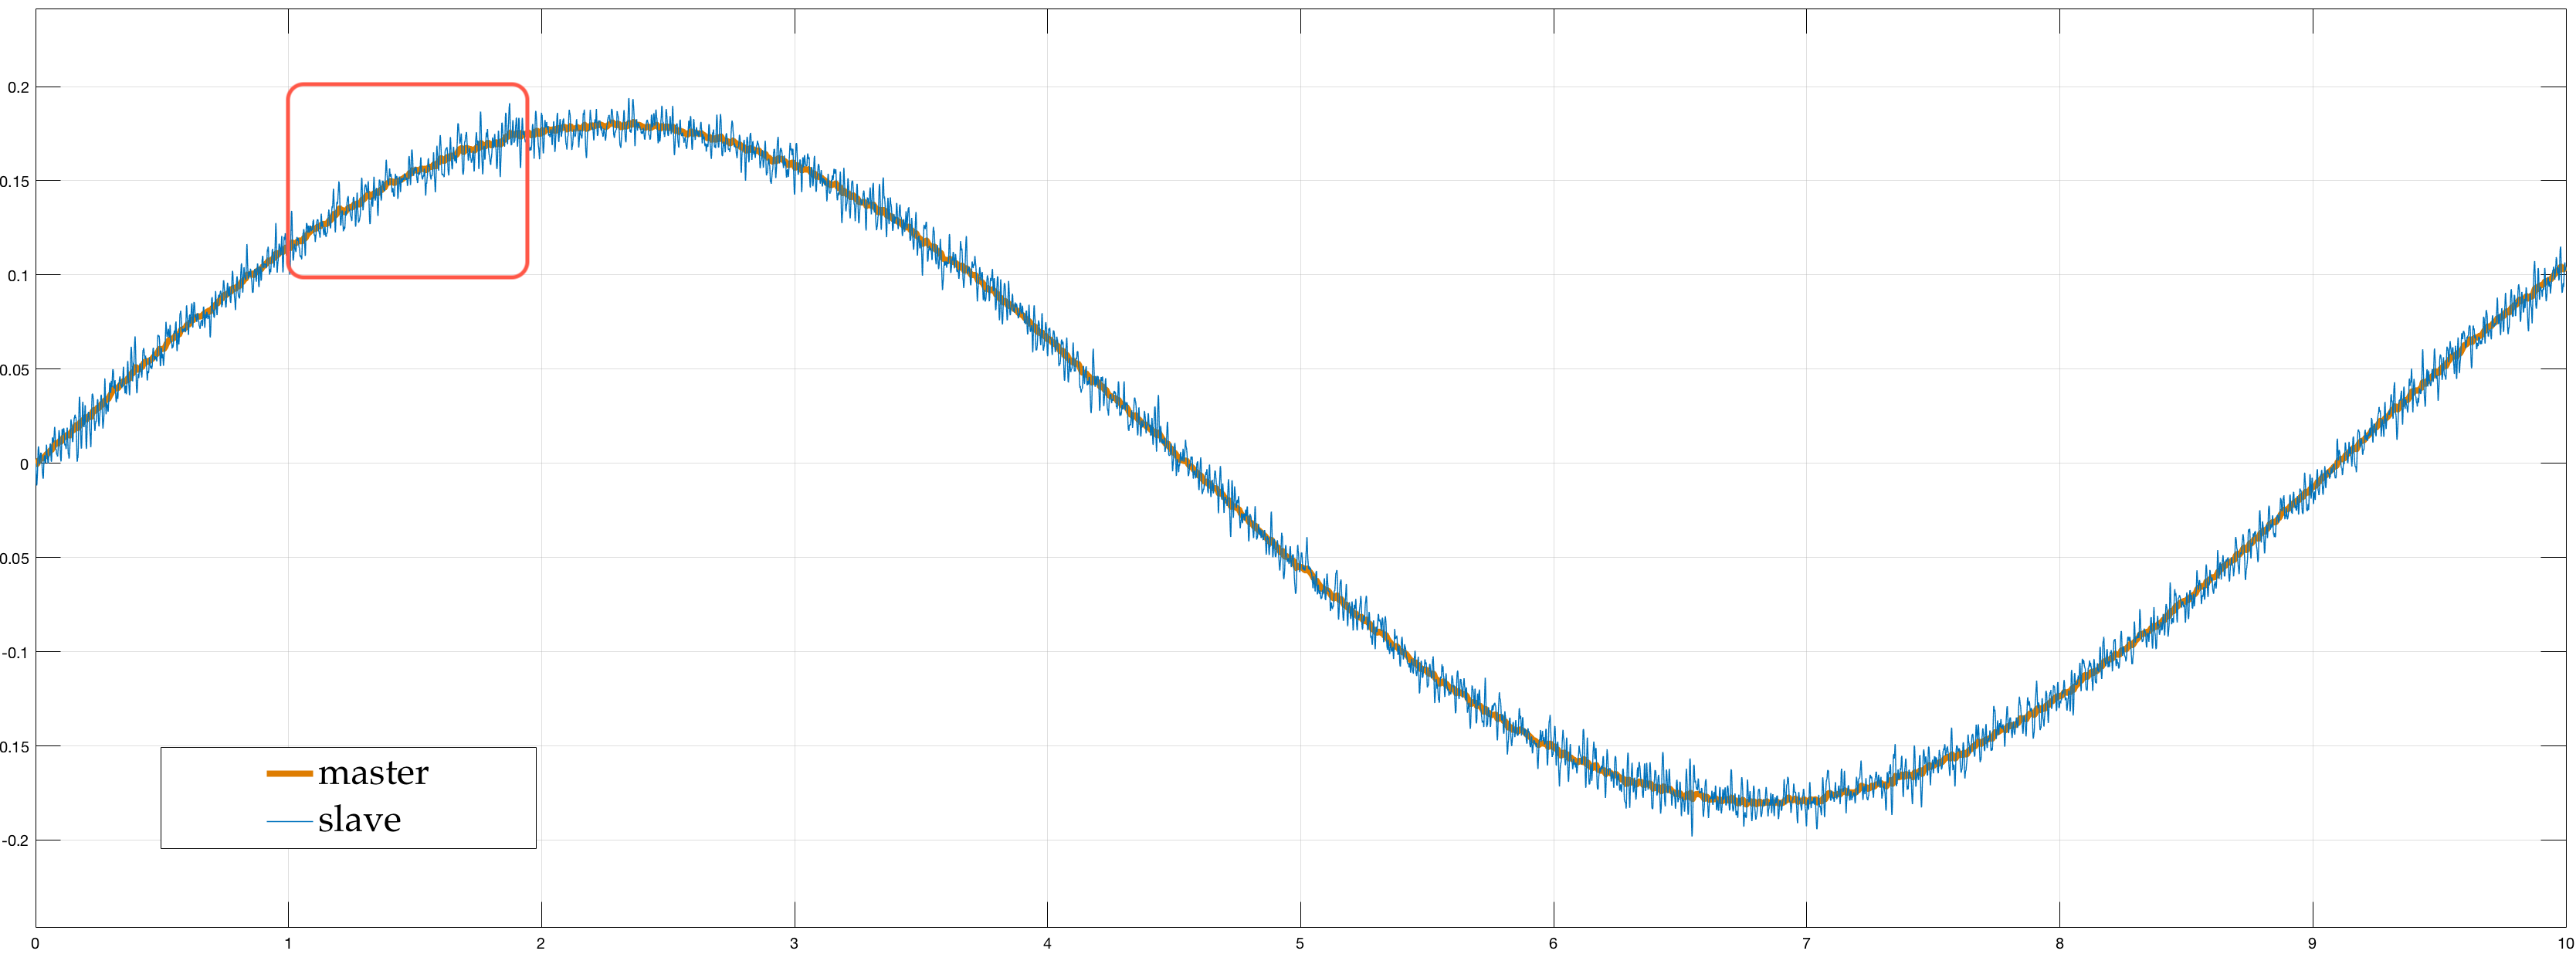
\includegraphics[width=1\linewidth]{Images/rCoupFreeTot50htznoiseRect}
% 	\caption{bodo}
% 	\label{fig:freeRigTot50HR}
% \end{figure}

% \begin{figure}[h]
% 	\centering
% 	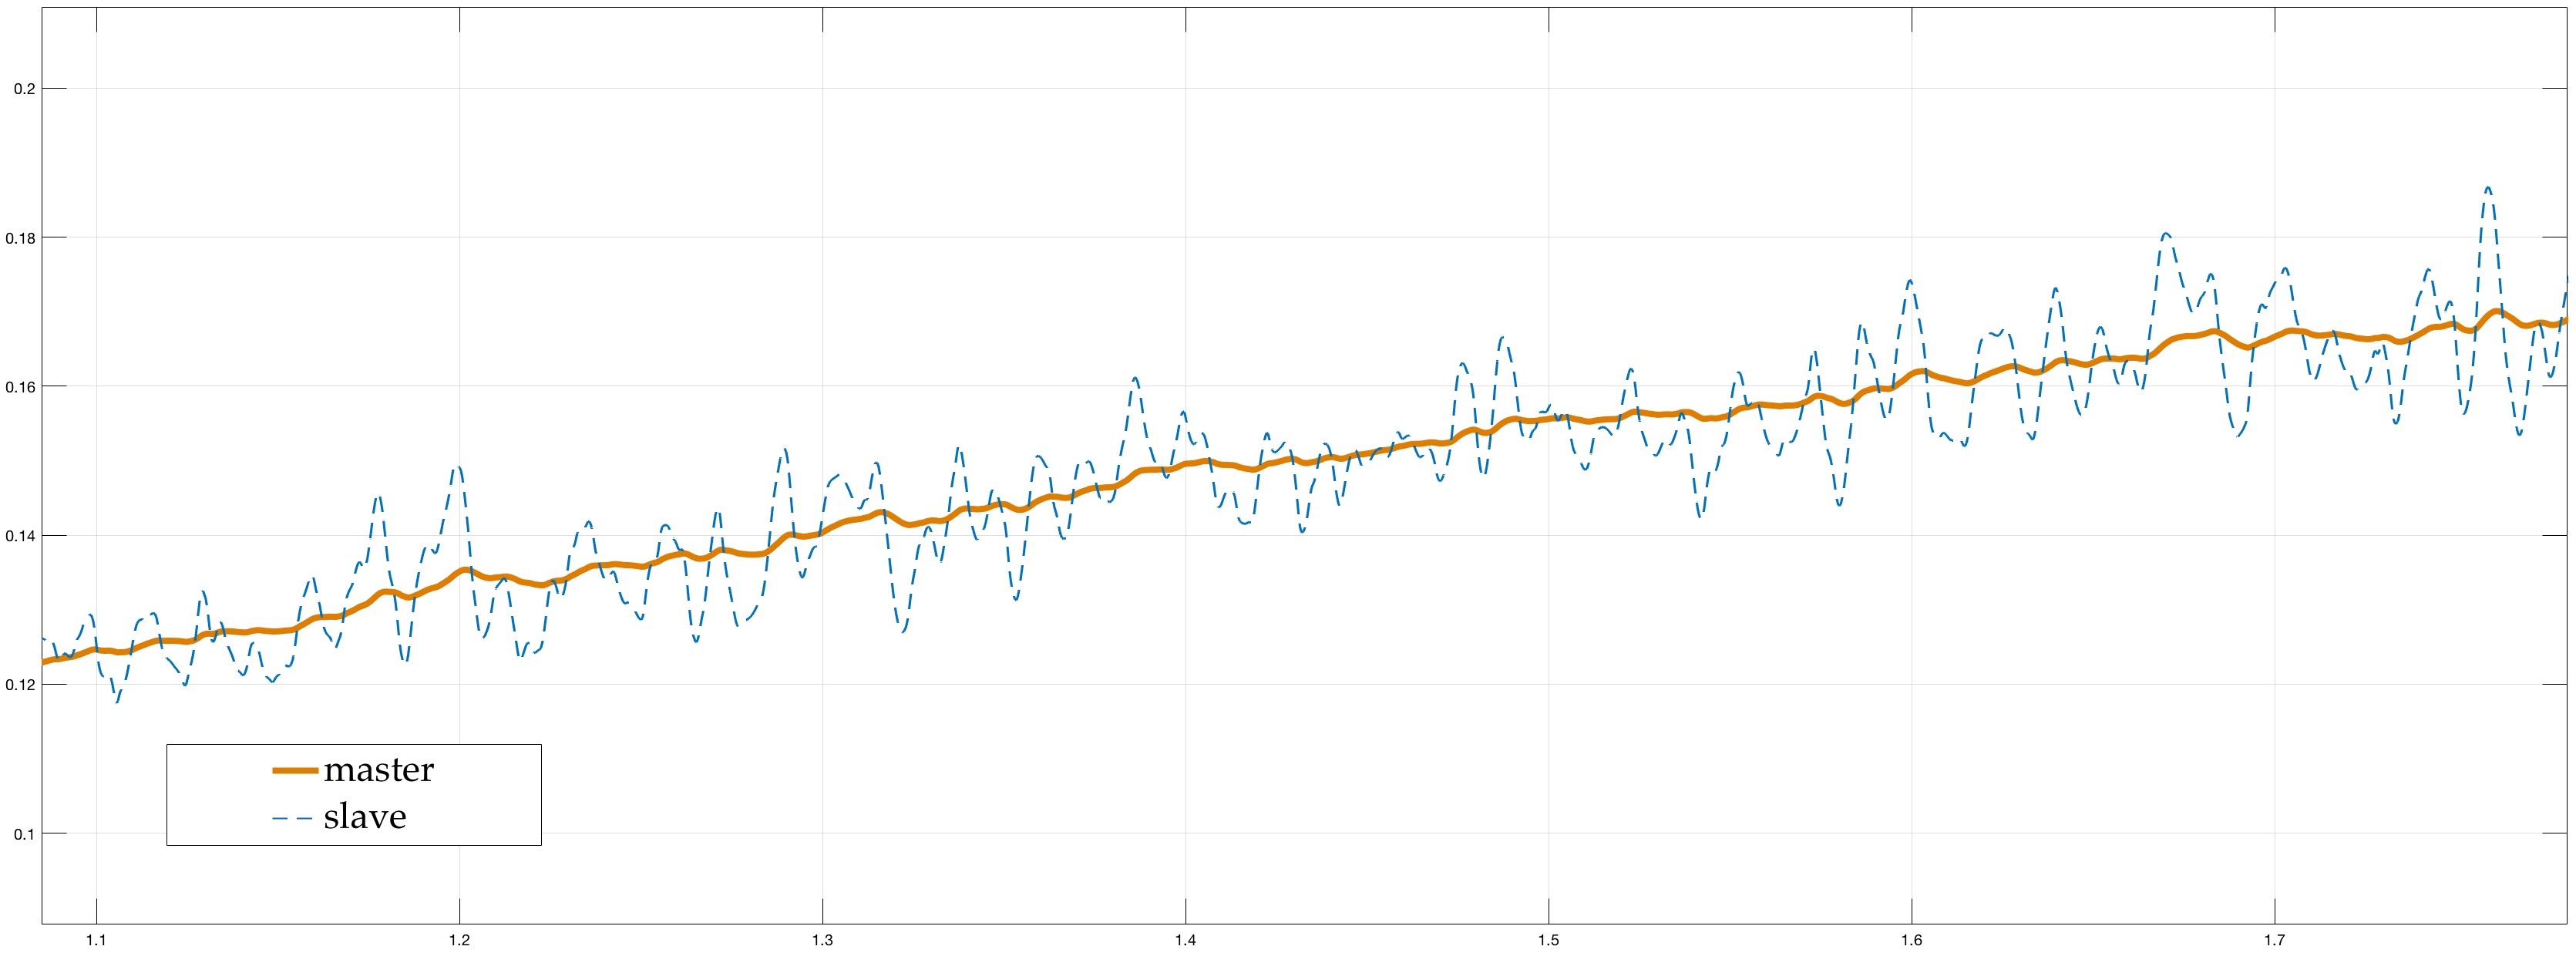
\includegraphics[width=1\linewidth]{Images/rCoupFree50htznoise}
% 	\caption{bodo}
% 	\label{fig:freeRigPar50HR}
% \end{figure}

% \begin{figure}[h]
% 	\centering
% 	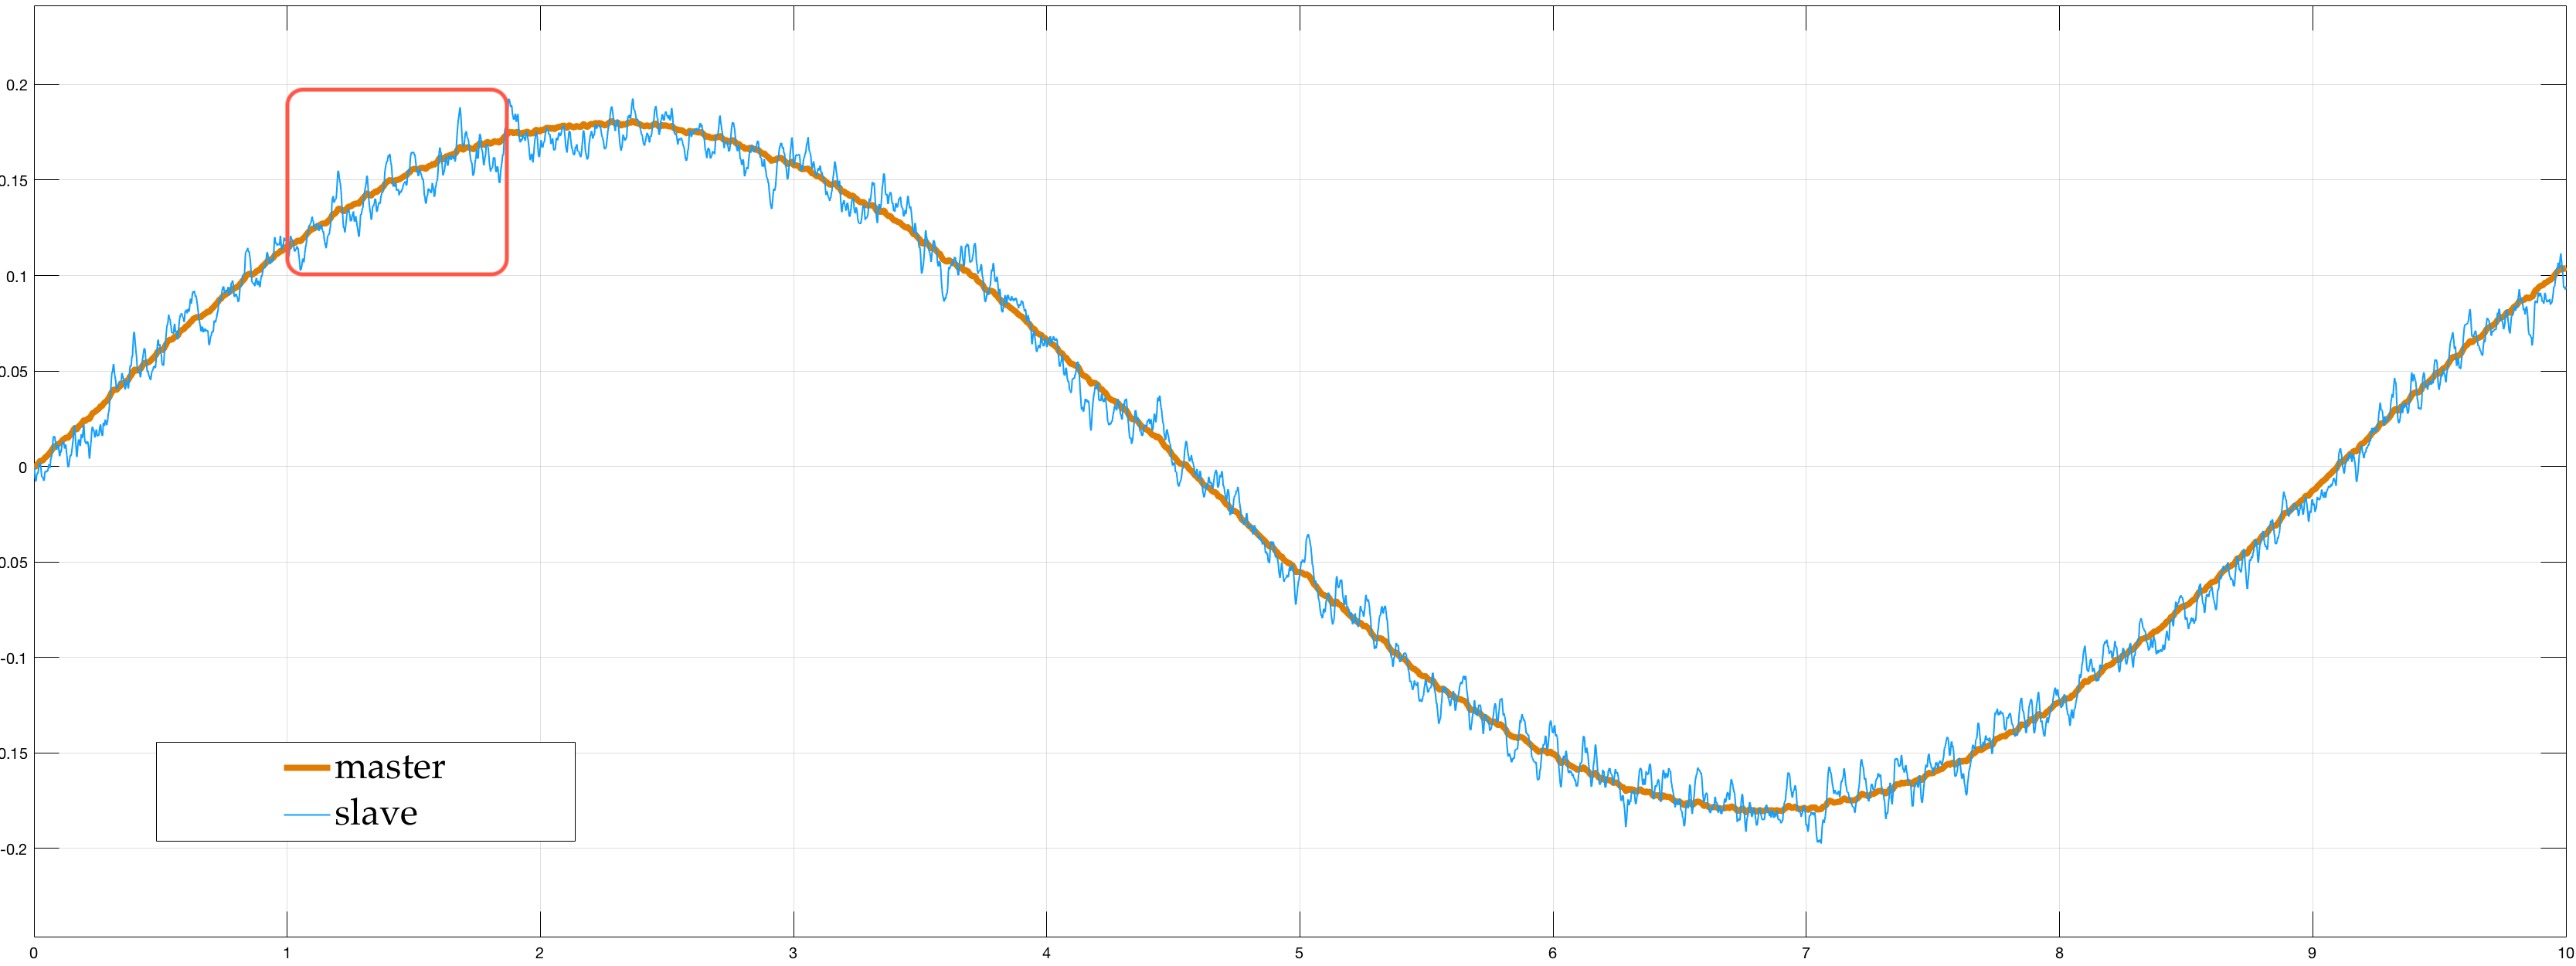
\includegraphics[width=1\linewidth]{Images/set20freeTot50HtznoiseRect}
% 	\caption{bodo}
% 	\label{fig:freeSetTot50HR}
% \end{figure}

% \begin{figure}[h]
% 	\centering
% 	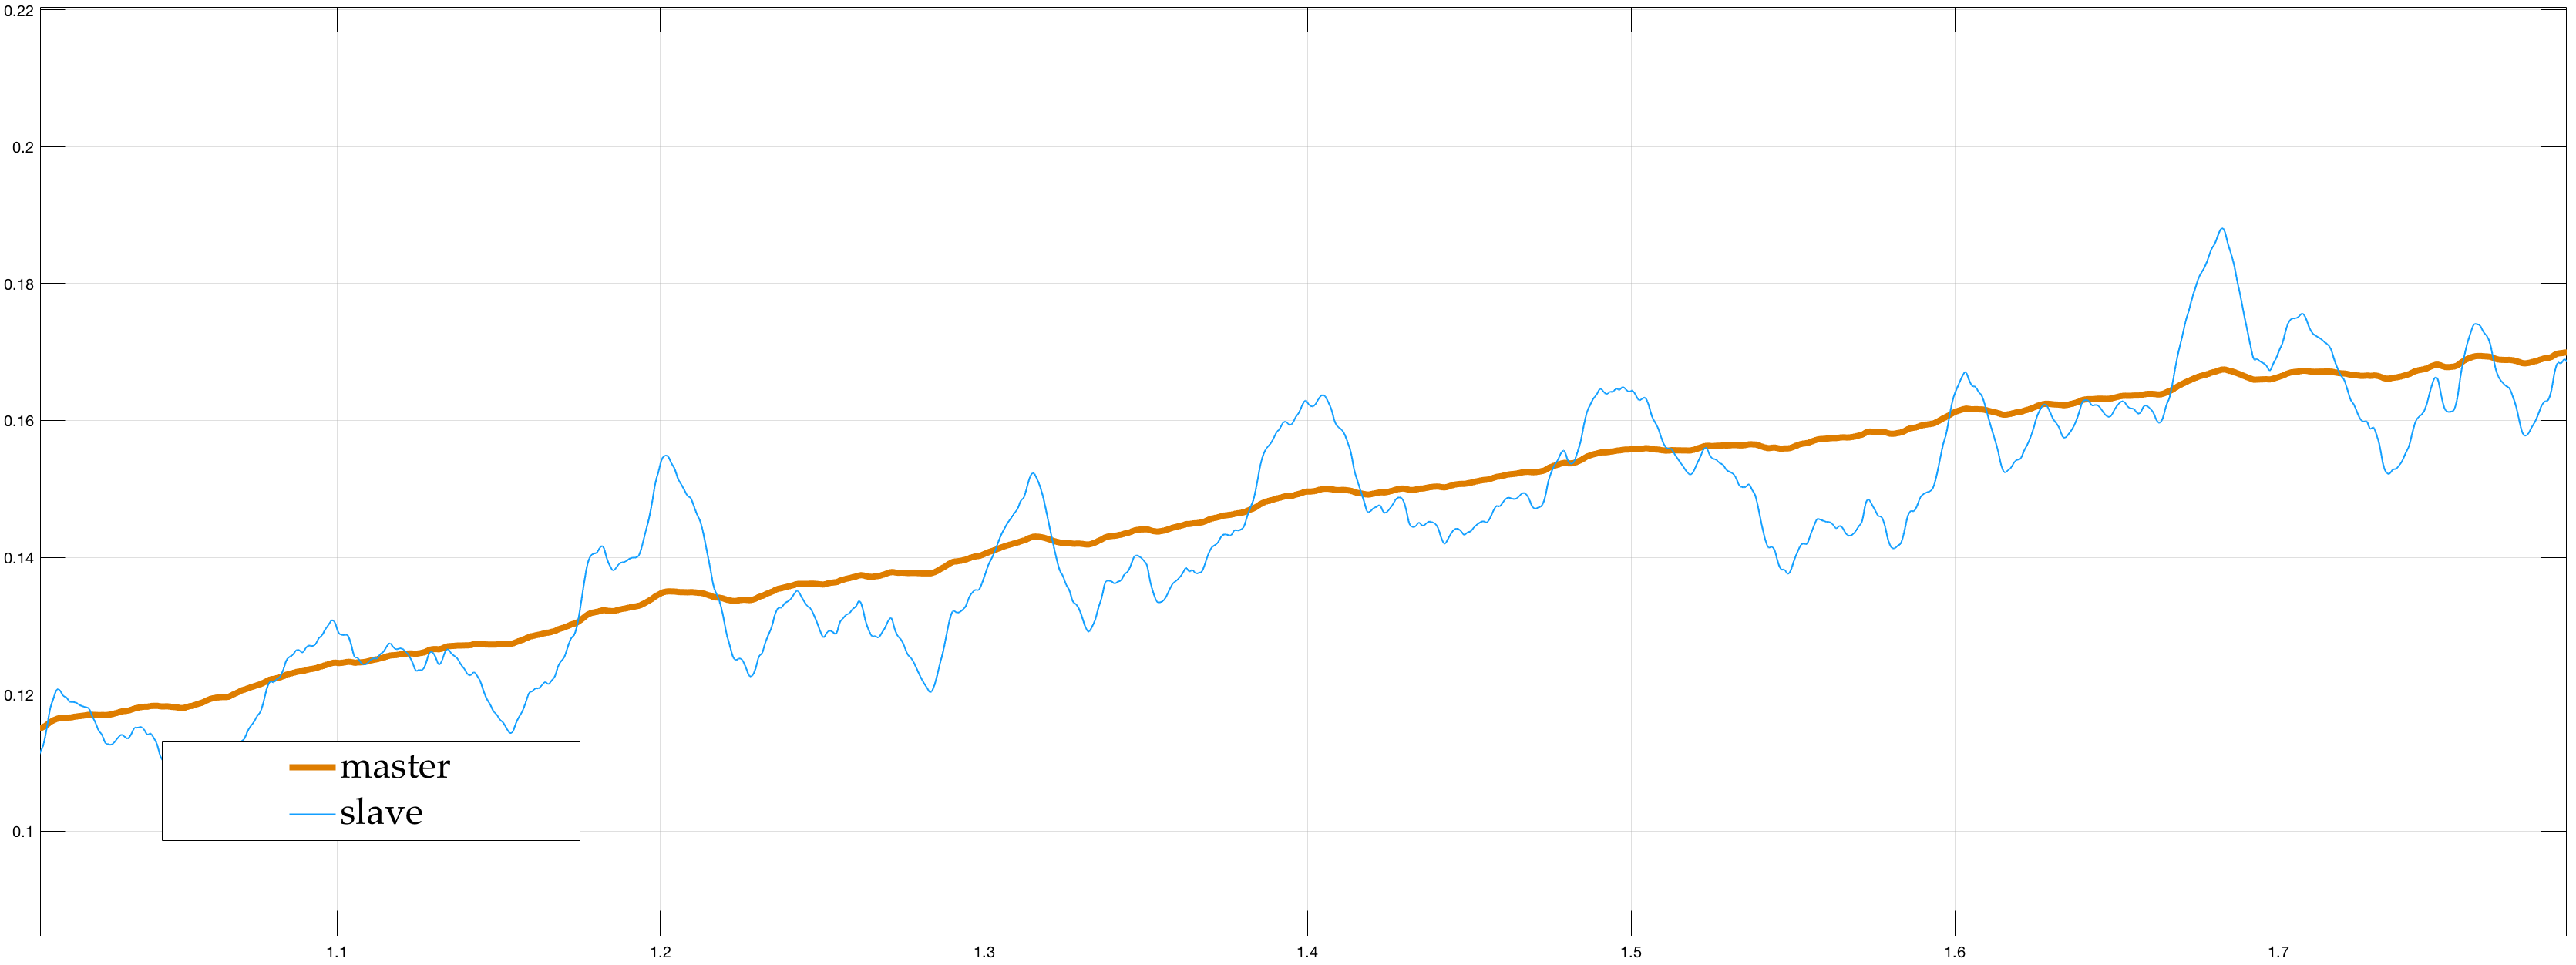
\includegraphics[width=1\linewidth]{Images/set20freePart50Htznoise}
% 	\caption{bodo}
% 	\label{fig:freeSetPar50HR}
% \end{figure}

% \begin{figure}[h]
% 	\centering
% 	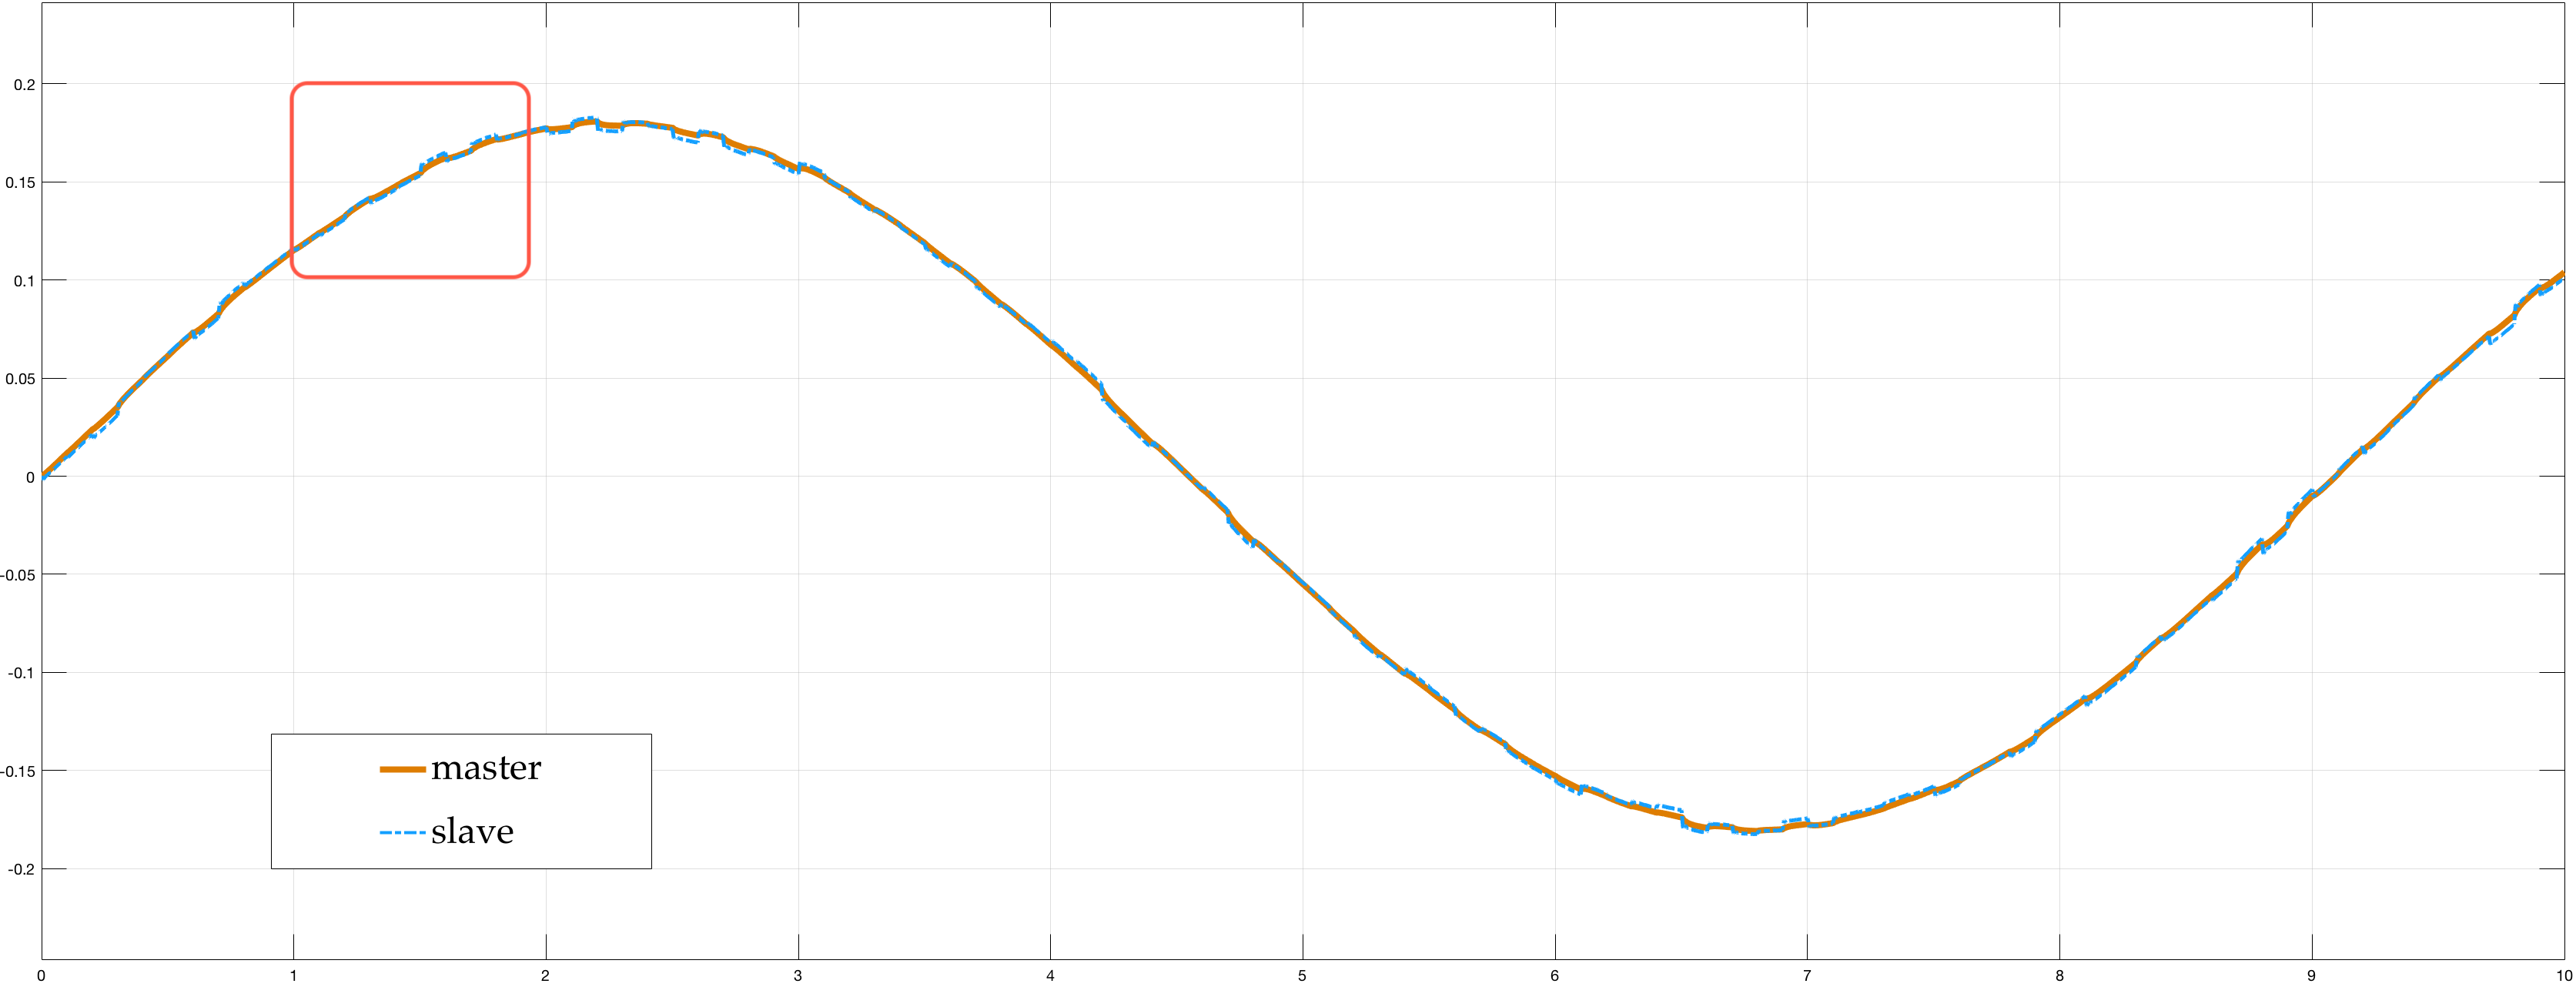
\includegraphics[width=1\linewidth]{Images/freerigidTot20HtznoiseRect}
% 	\caption{bodo}
% 	\label{fig:freeRigTot20HR}
% \end{figure}

% \begin{figure}[h]
% 	\centering
% 	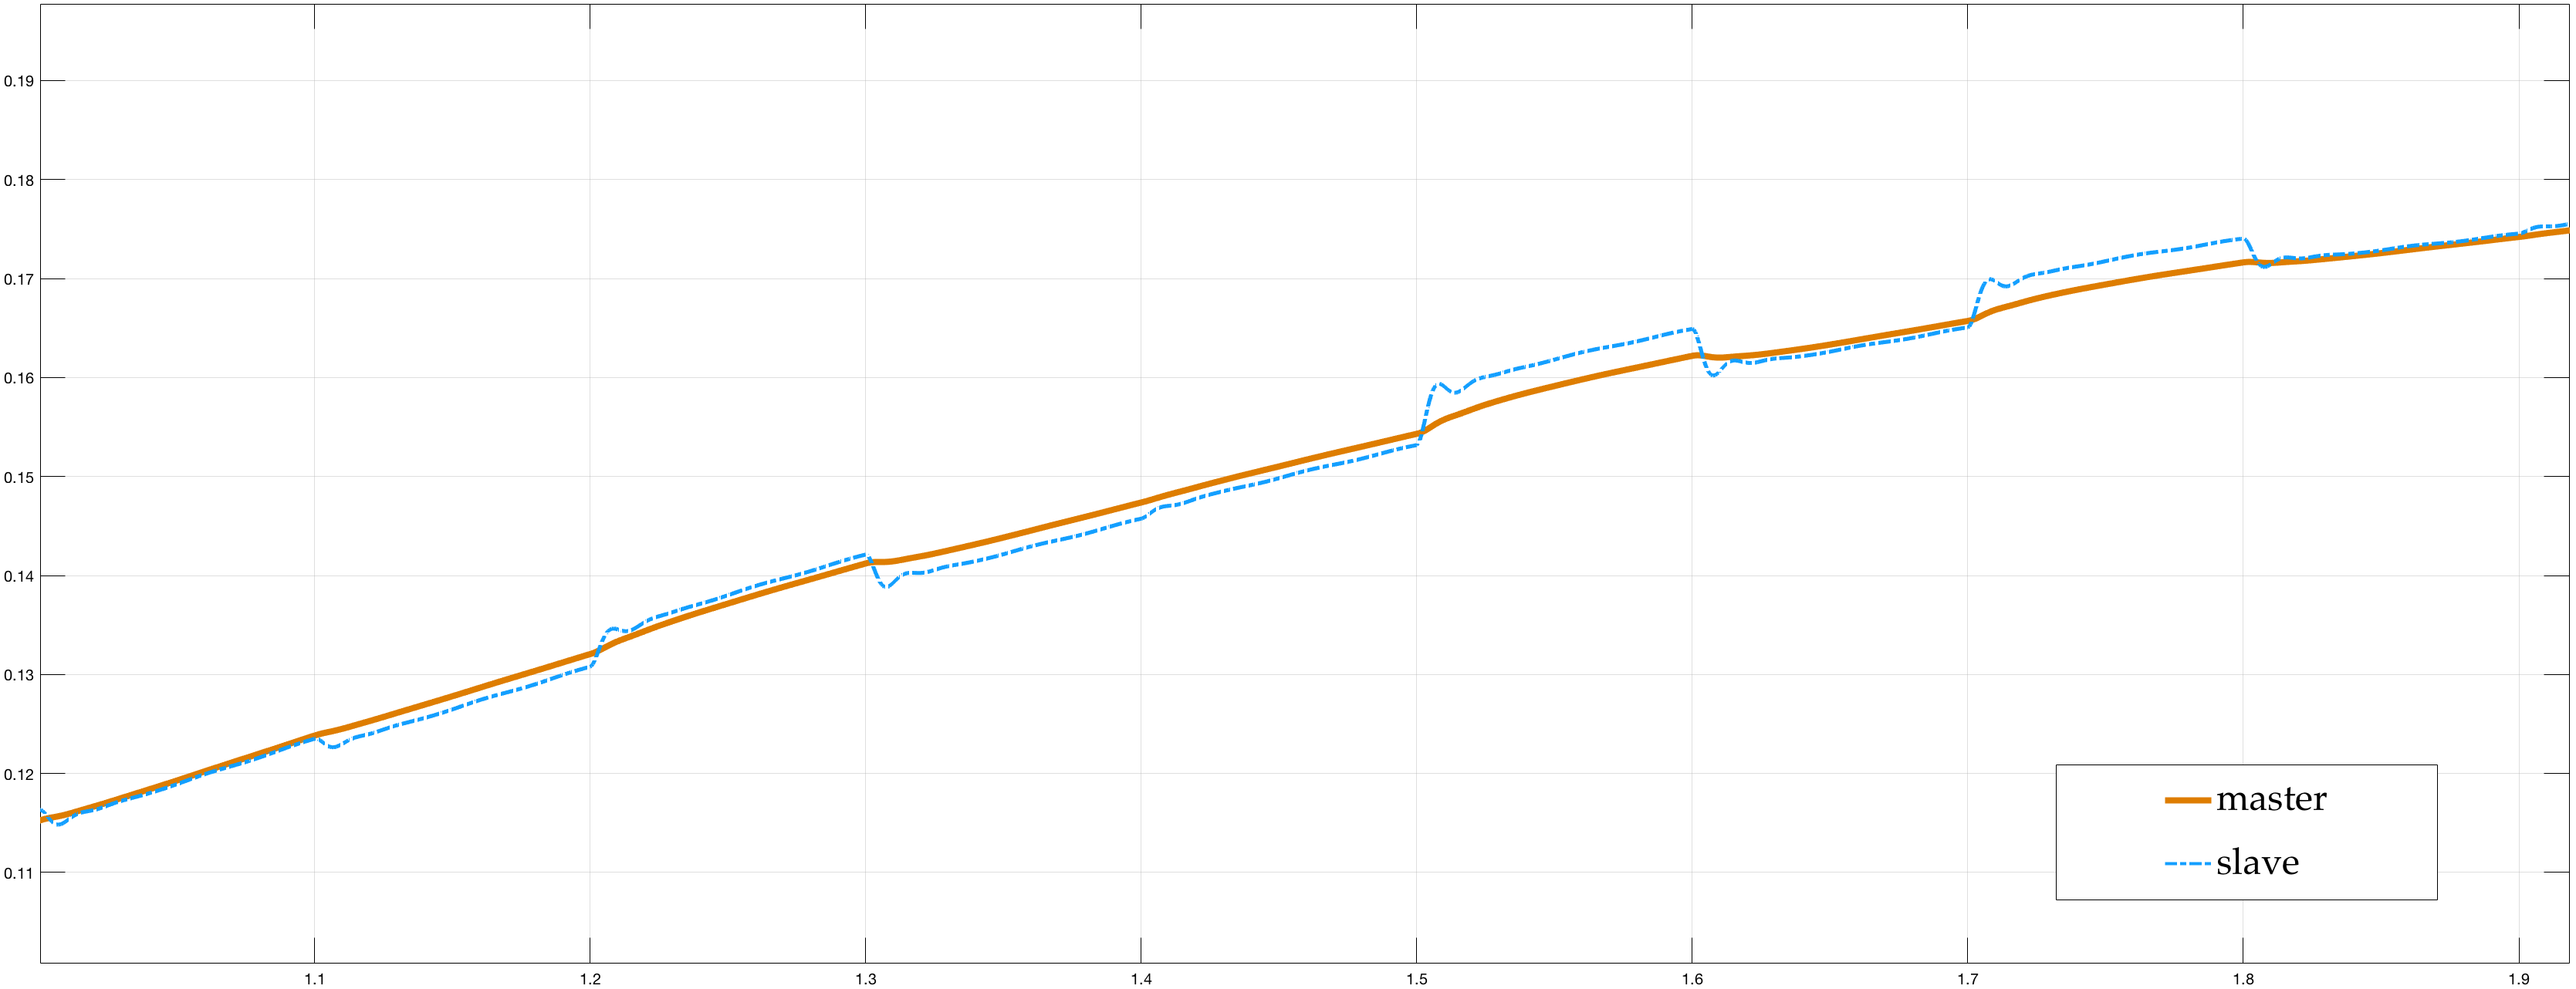
\includegraphics[width=1\linewidth]{Images/freerigidPart20Htznoise}
% 	\caption{bodo}
% 	\label{fig:freeRigPar20HR}
% \end{figure}

% \begin{figure}[h]
% 	\centering
% 	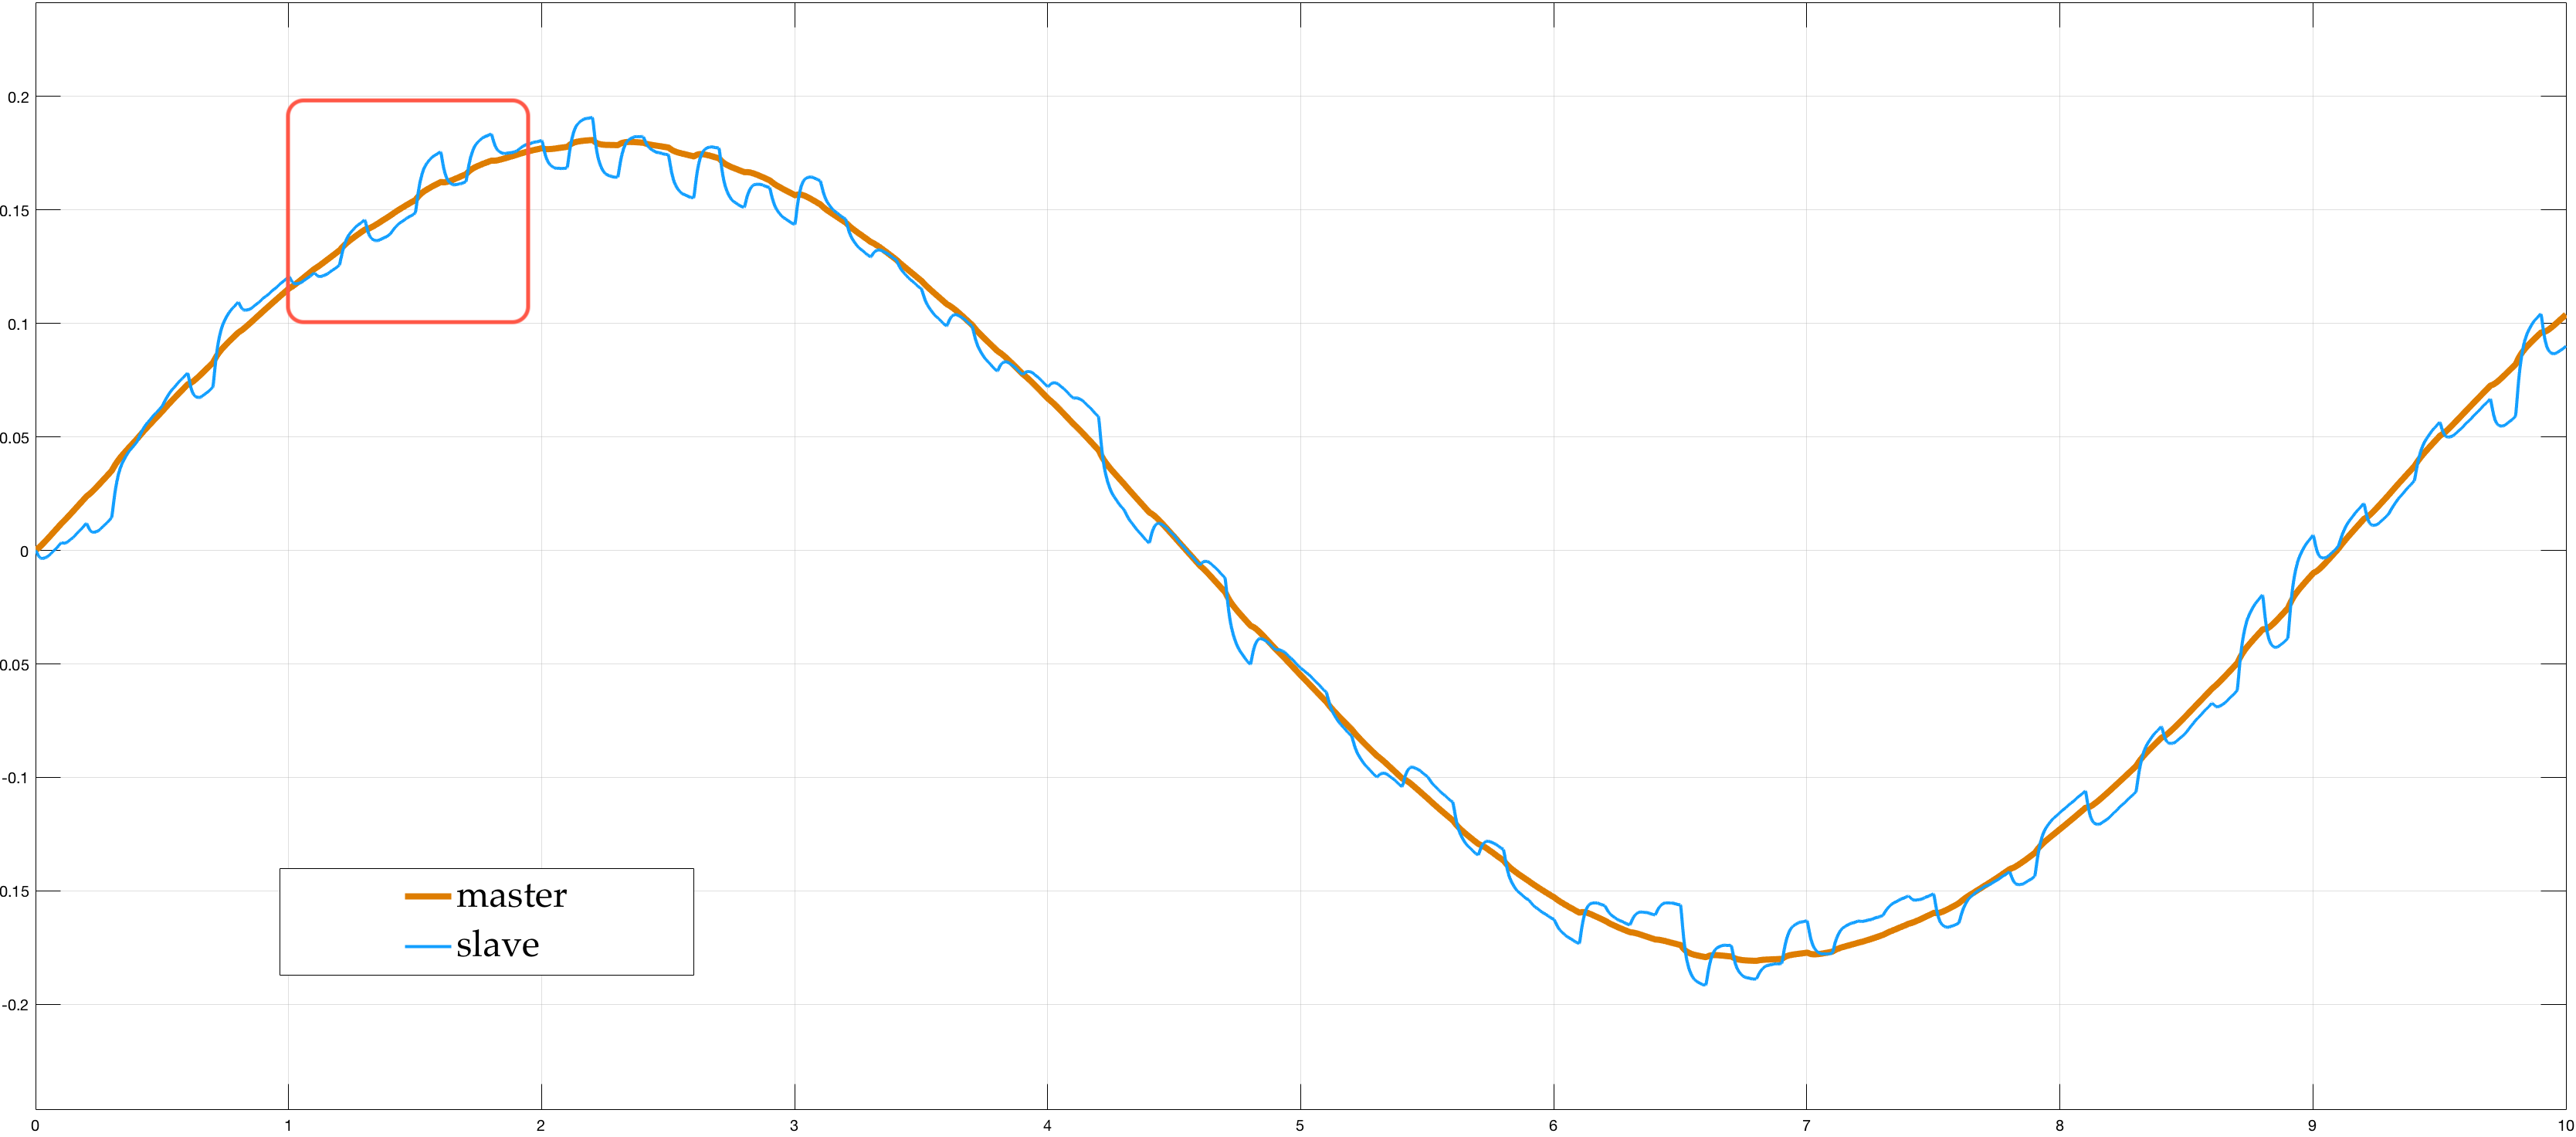
\includegraphics[width=1\linewidth]{Images/freeSet20Tot20HtznoiseRect}
% 	\caption{bodo}
% 	\label{fig:freeSetTot20HR}
% \end{figure}

% \begin{figure}[h]
% 	\centering
% 	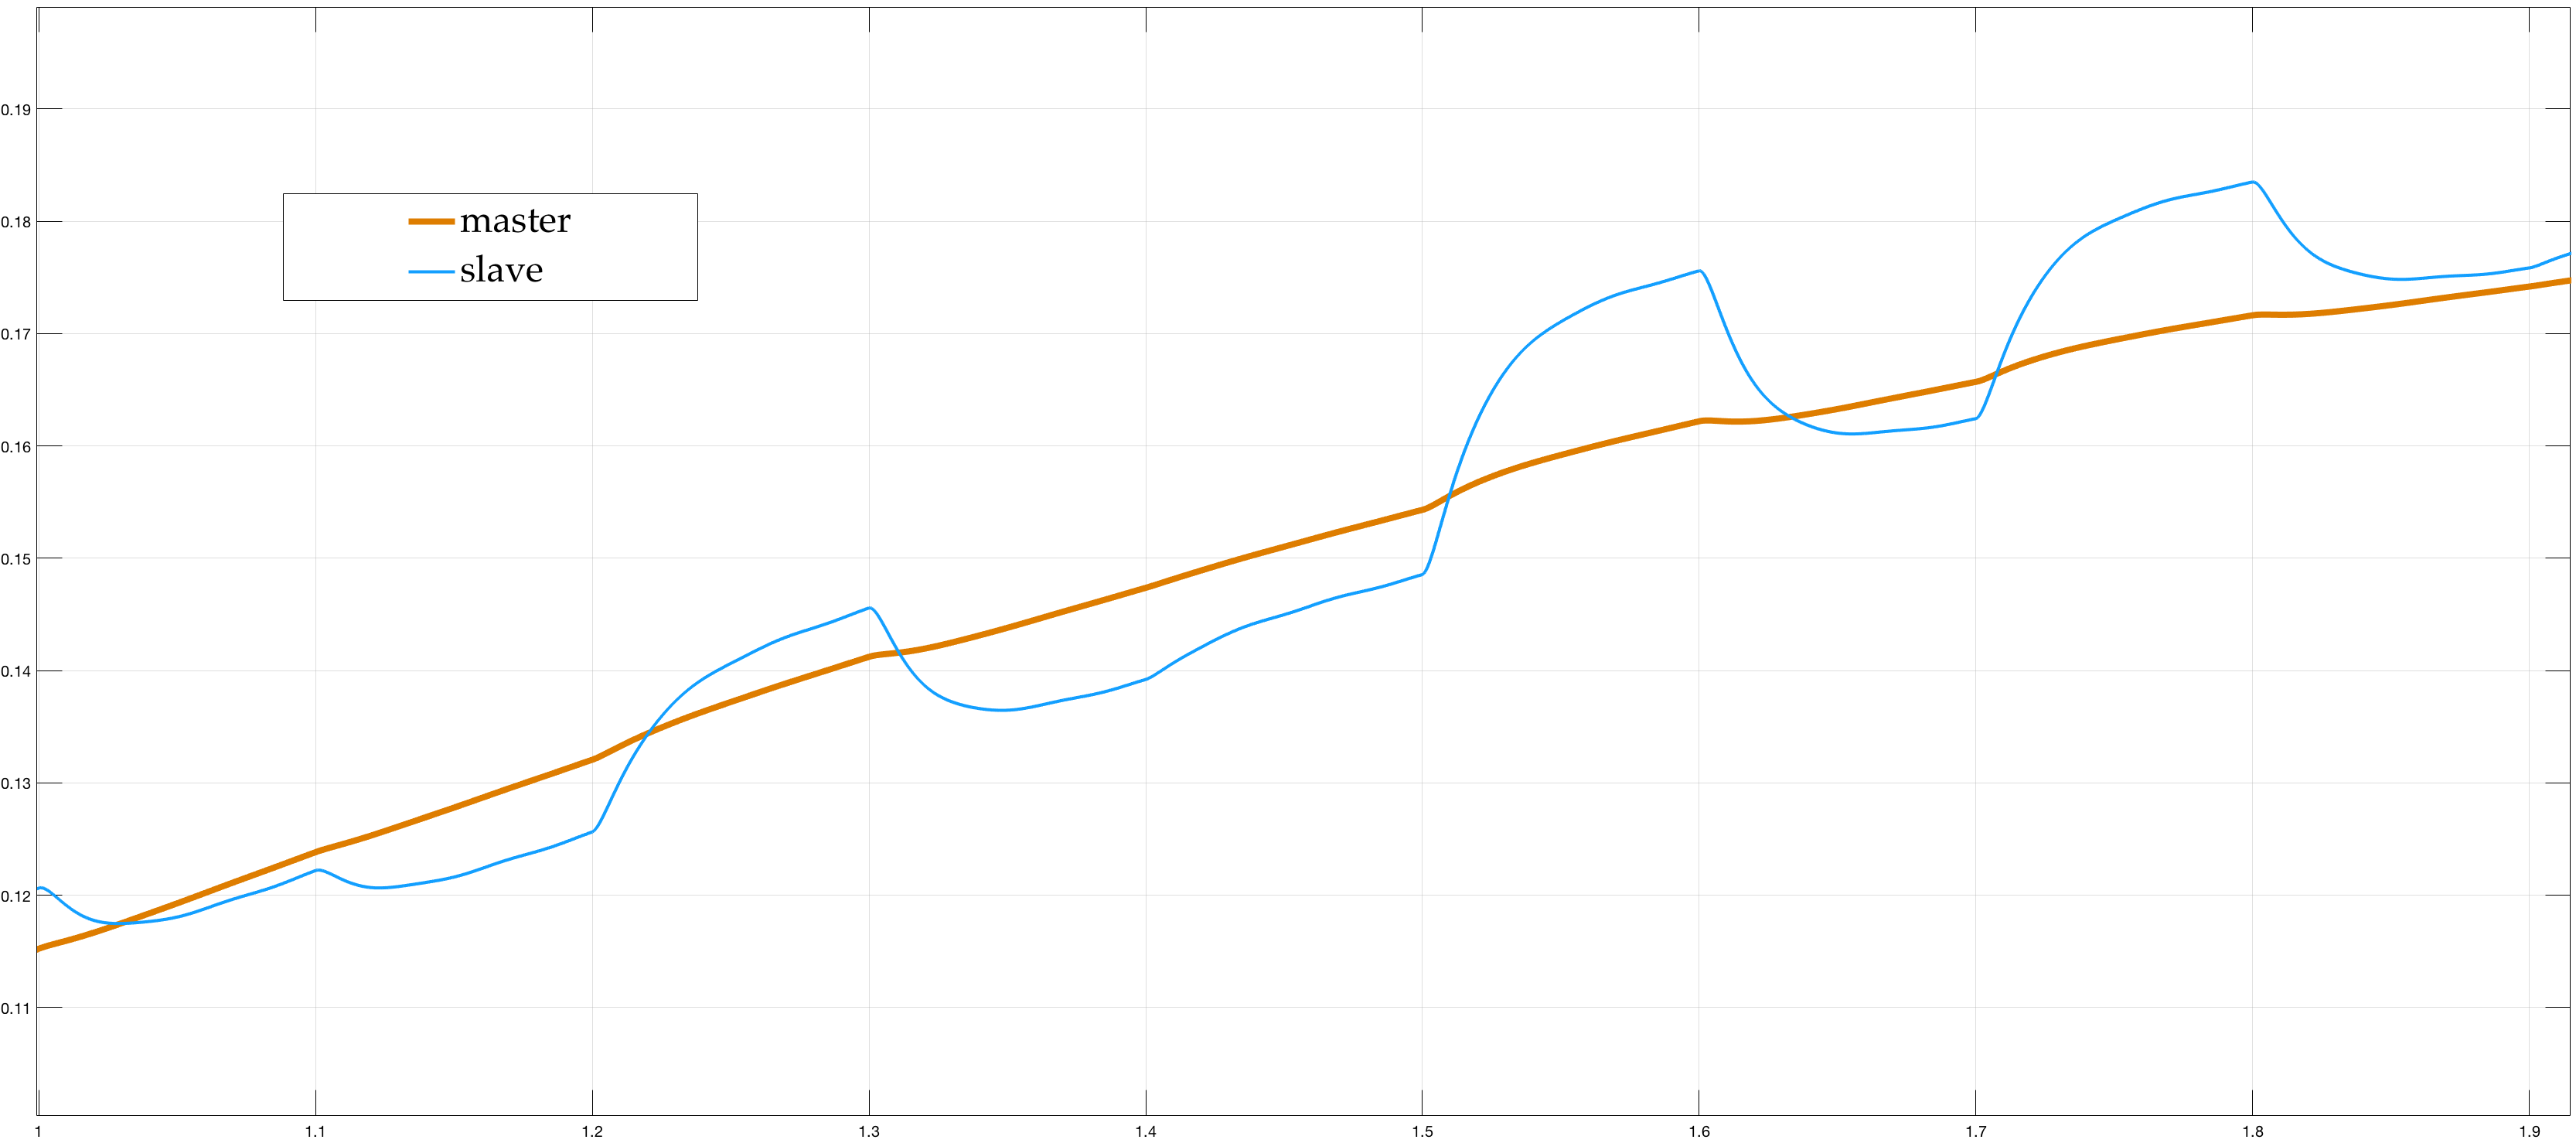
\includegraphics[width=1\linewidth]{Images/freeSet20Part20Htznoise}
% 	\caption{bodo}
% 	\label{fig:freeSetPar20HR}
% \end{figure}




\begin{figure}
	\begin{subfigure}[h!]{1\linewidth}
		\centering
		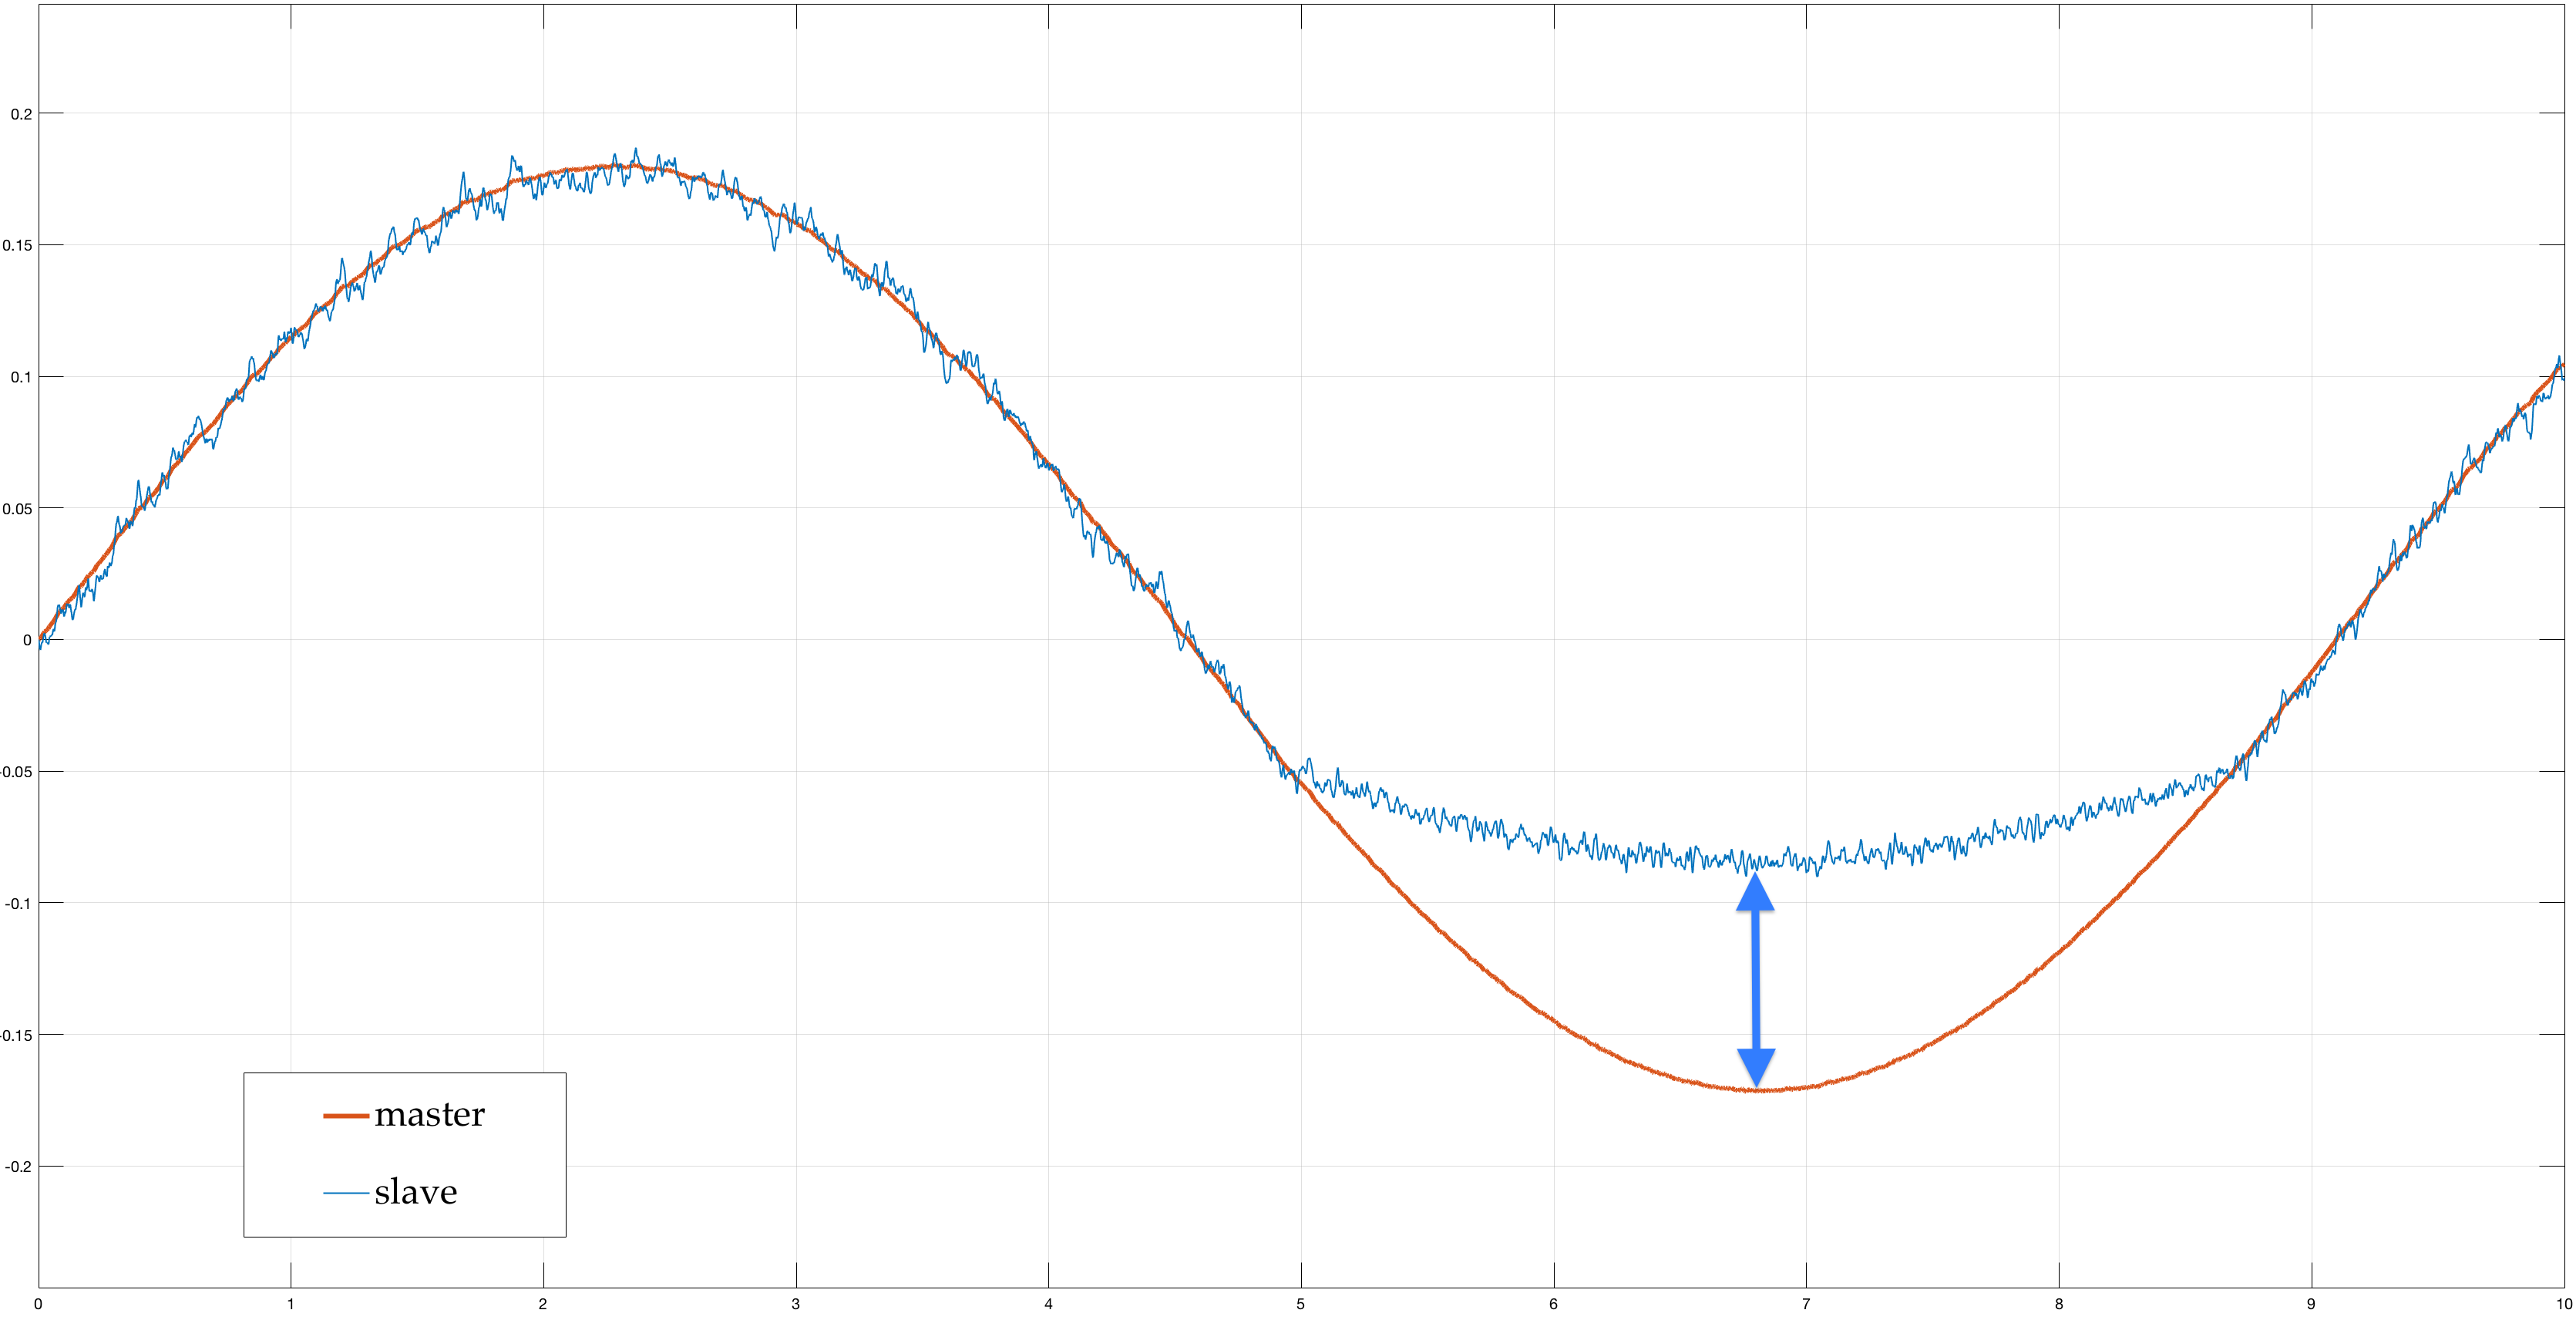
\includegraphics[width=\textwidth, height=\textwidth/2]{Images/setPointContactReacPosArrow}
		\caption{ ffff}
		\label{fig:ContactSetPos}
	\end{subfigure}	
  \newline
	\begin{subfigure}[h!]{1\linewidth}
		\centering
		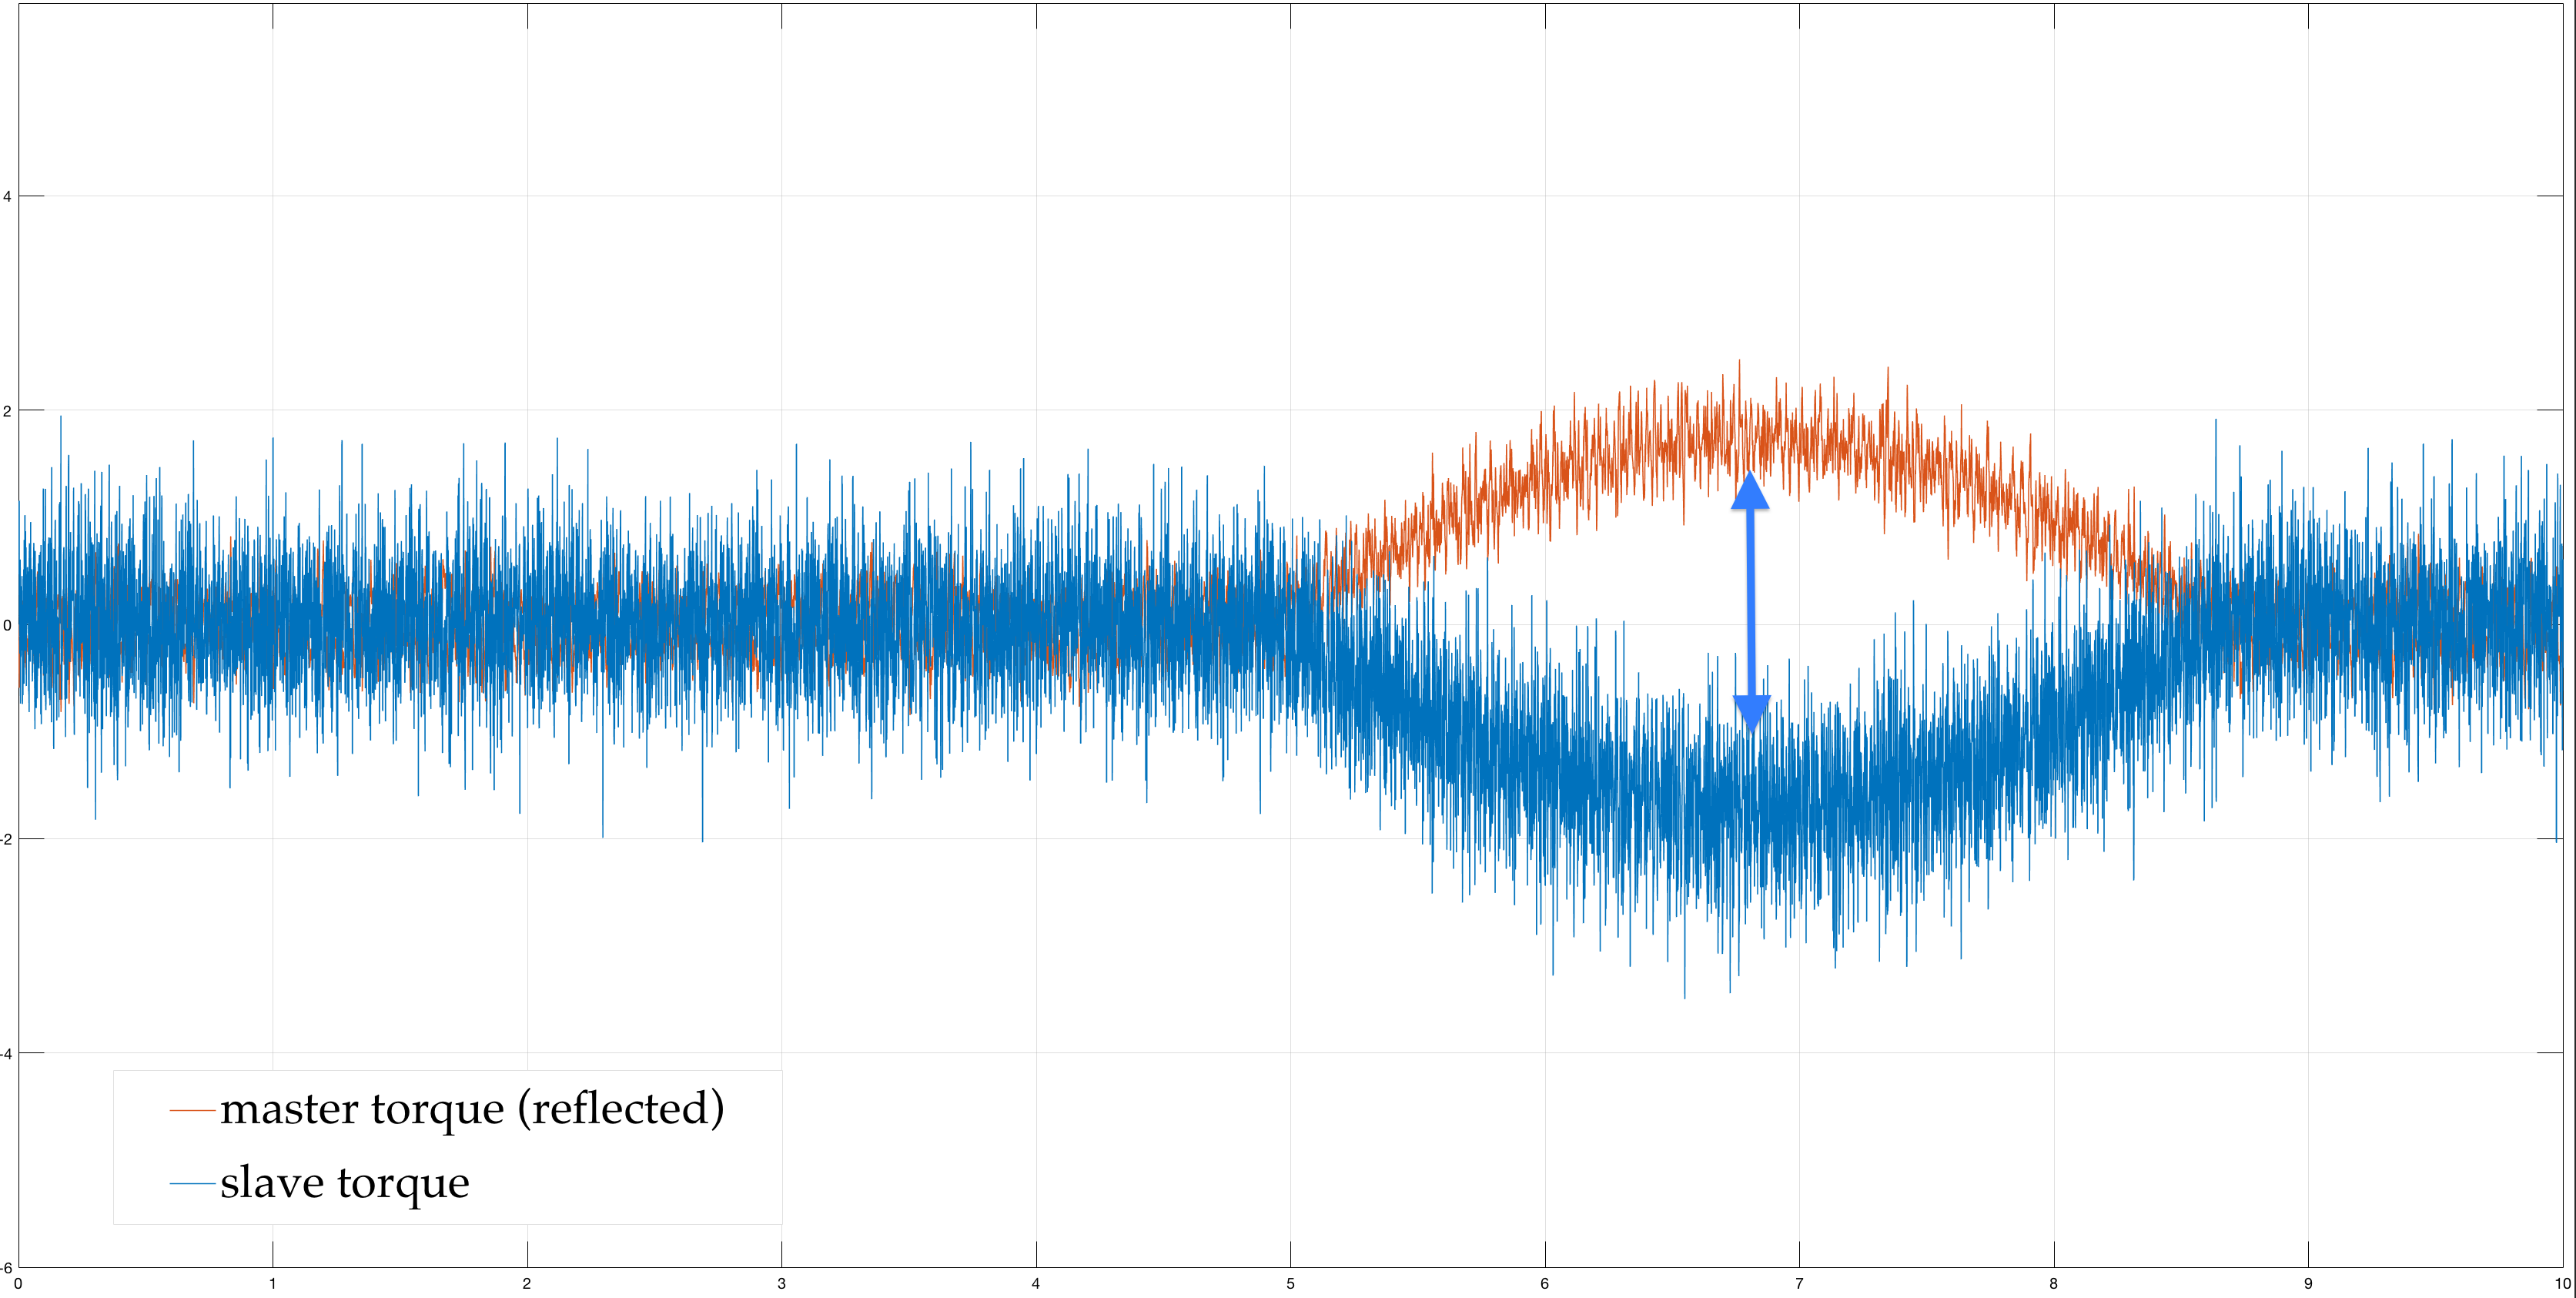
\includegraphics[width=\textwidth, height=\textwidth/2]{Images/setPointContactReacTorArrow}
		\caption{ ffff}
		\label{fig:ContactSetTor}
	\end{subfigure}	
 \caption{ fffff }
\end{figure}

\begin{figure}
	\begin{subfigure}[h!]{1\linewidth}
		\centering
		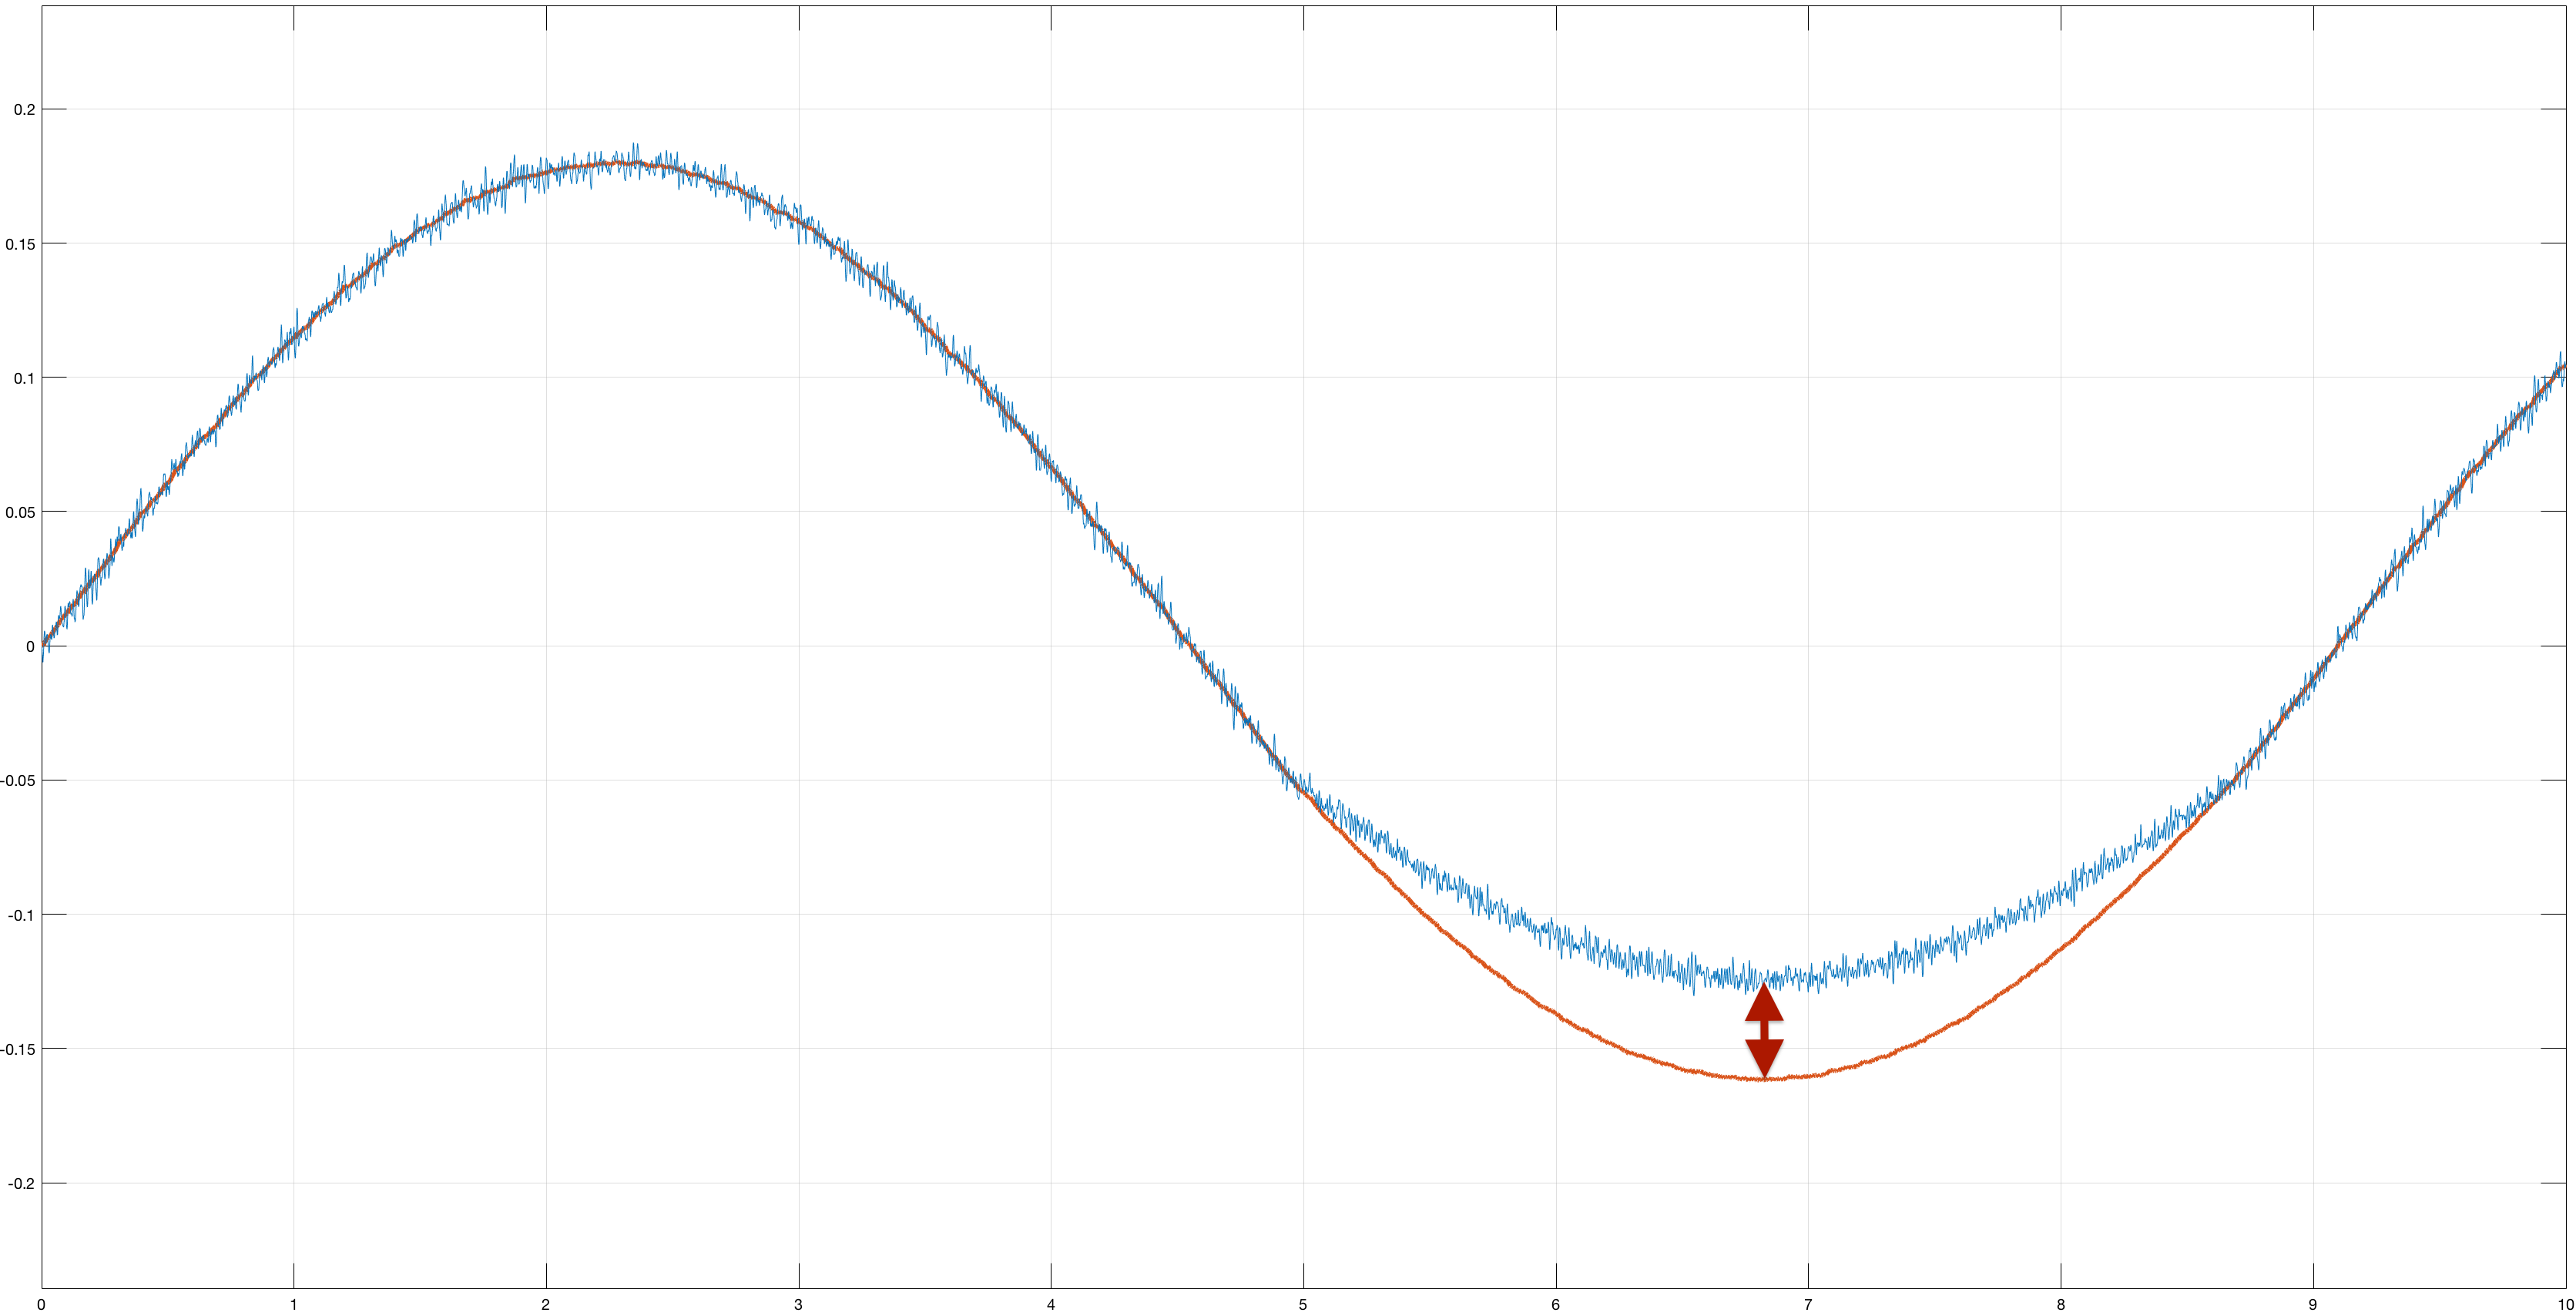
\includegraphics[width=\textwidth, height=\textwidth/2]{Images/rigidContactReacPosArrow}
		\caption{ ffff}
		\label{fig:ContactRigPos}
	\end{subfigure}	
  \newline
	\begin{subfigure}[h!]{1\linewidth}
		\centering
		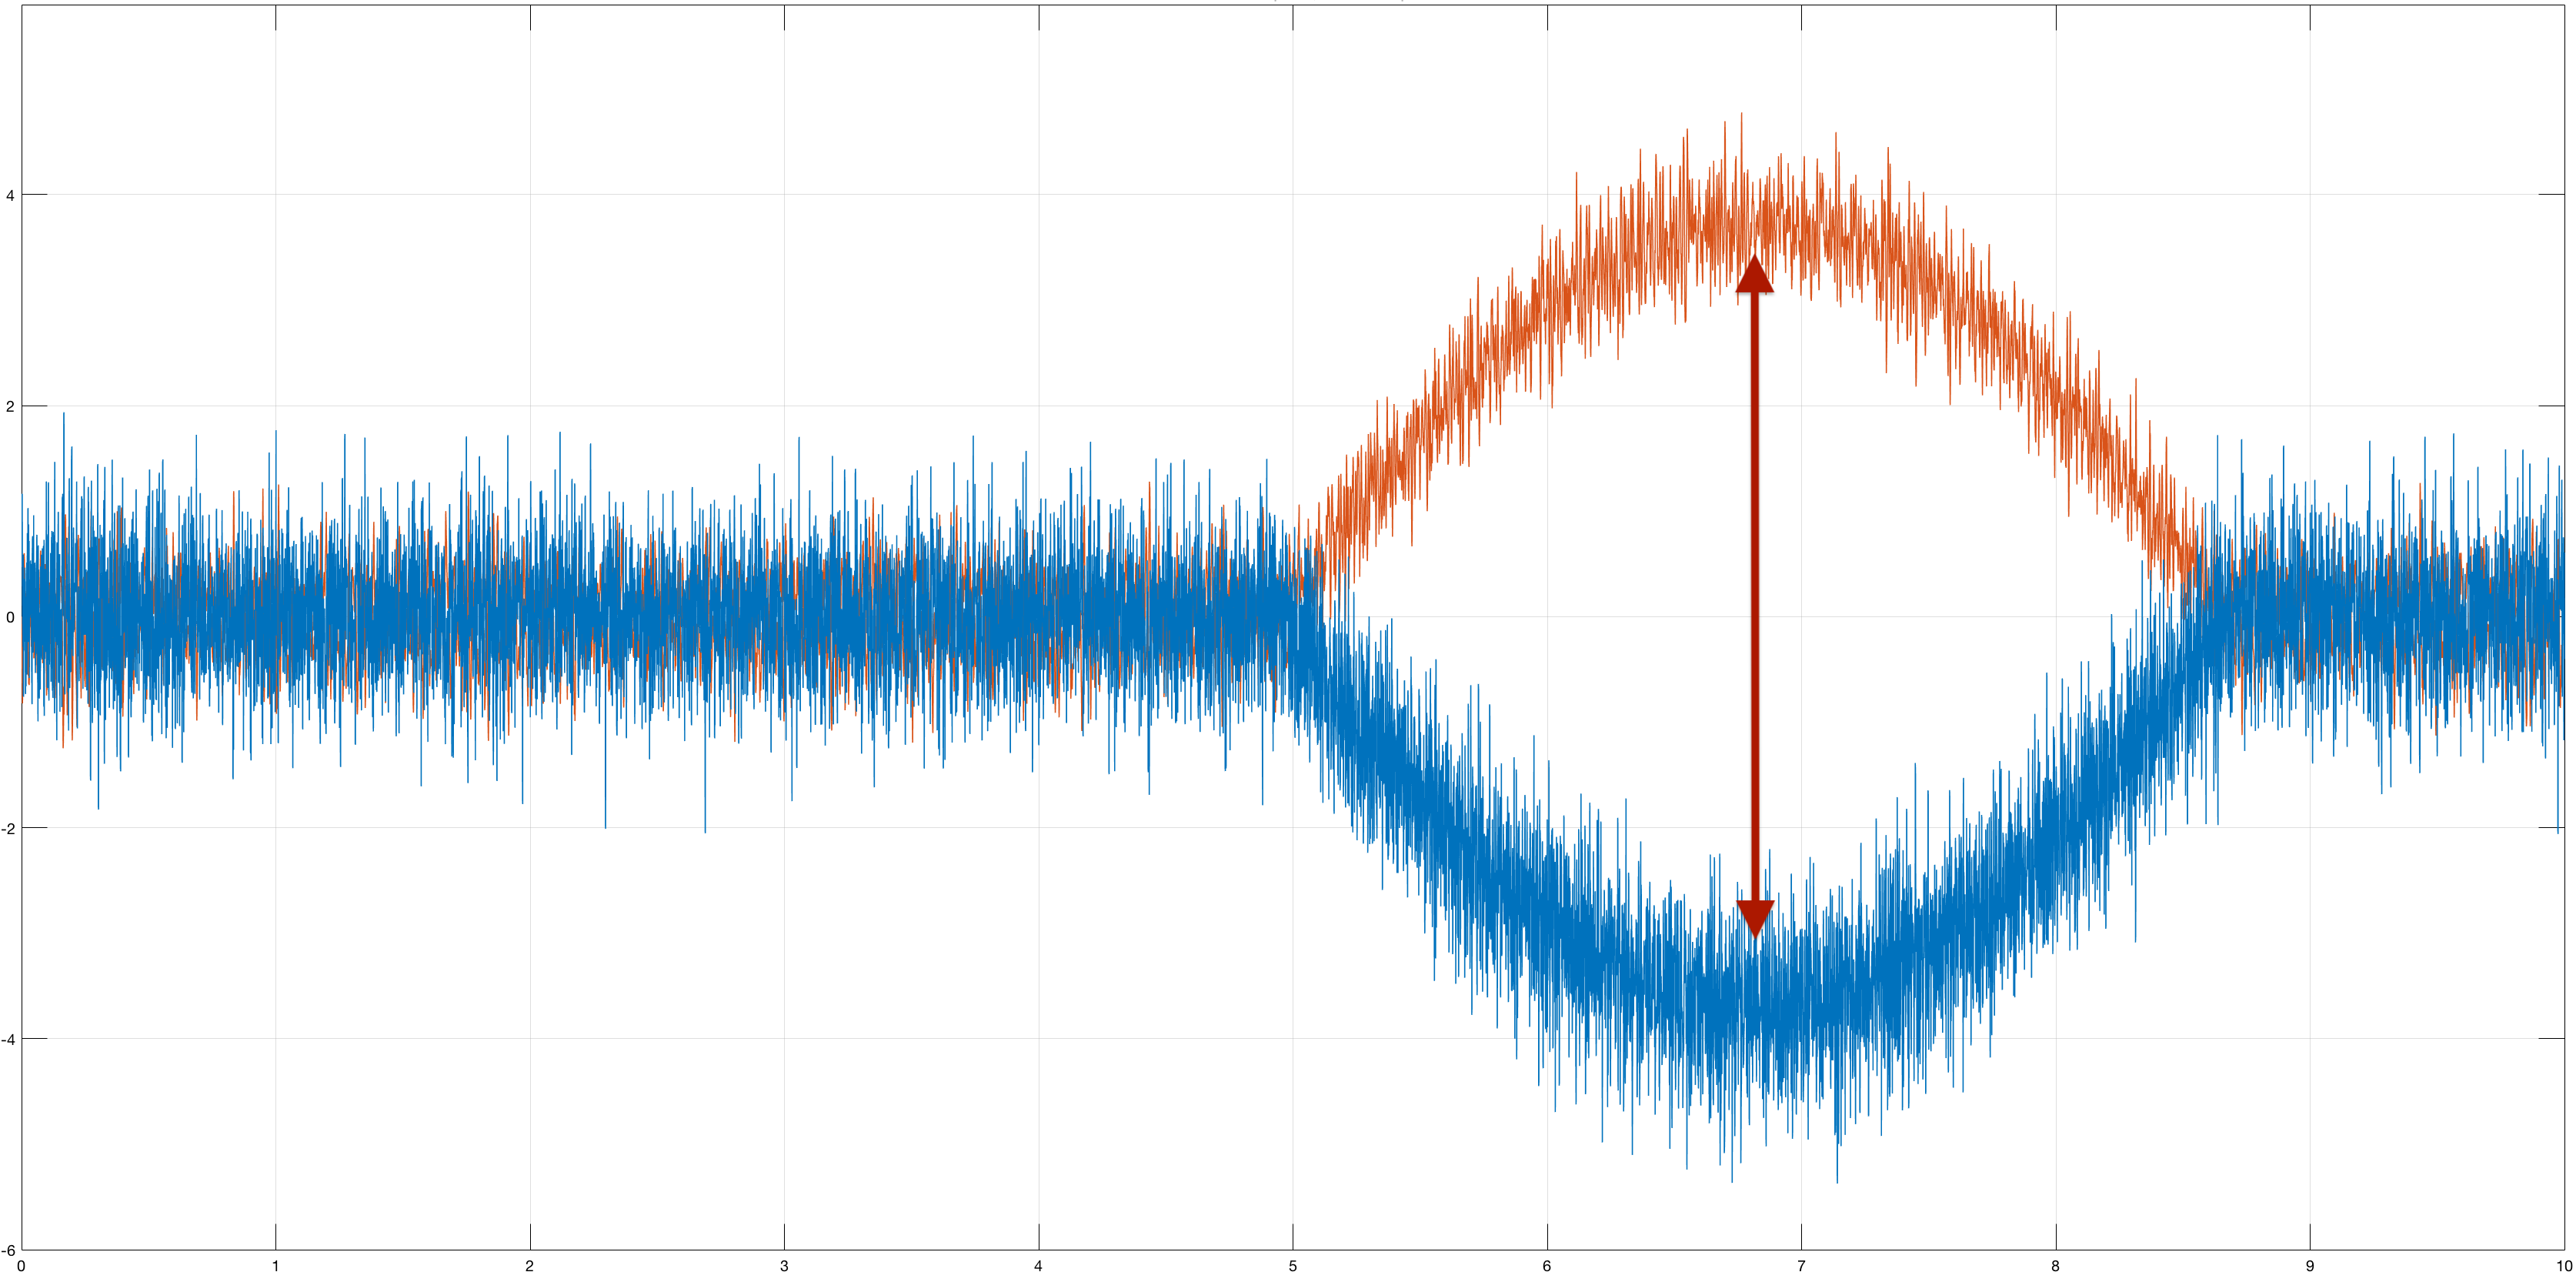
\includegraphics[width=\textwidth, height=\textwidth/2]{Images/rigidContactReacTorArrow}
		\caption{ ffff}
		\label{fig:ContactRigTor}
	\end{subfigure}	
 \caption{ fffff }
\end{figure}






% \begin{figure}[h]
% 	\centering
% 	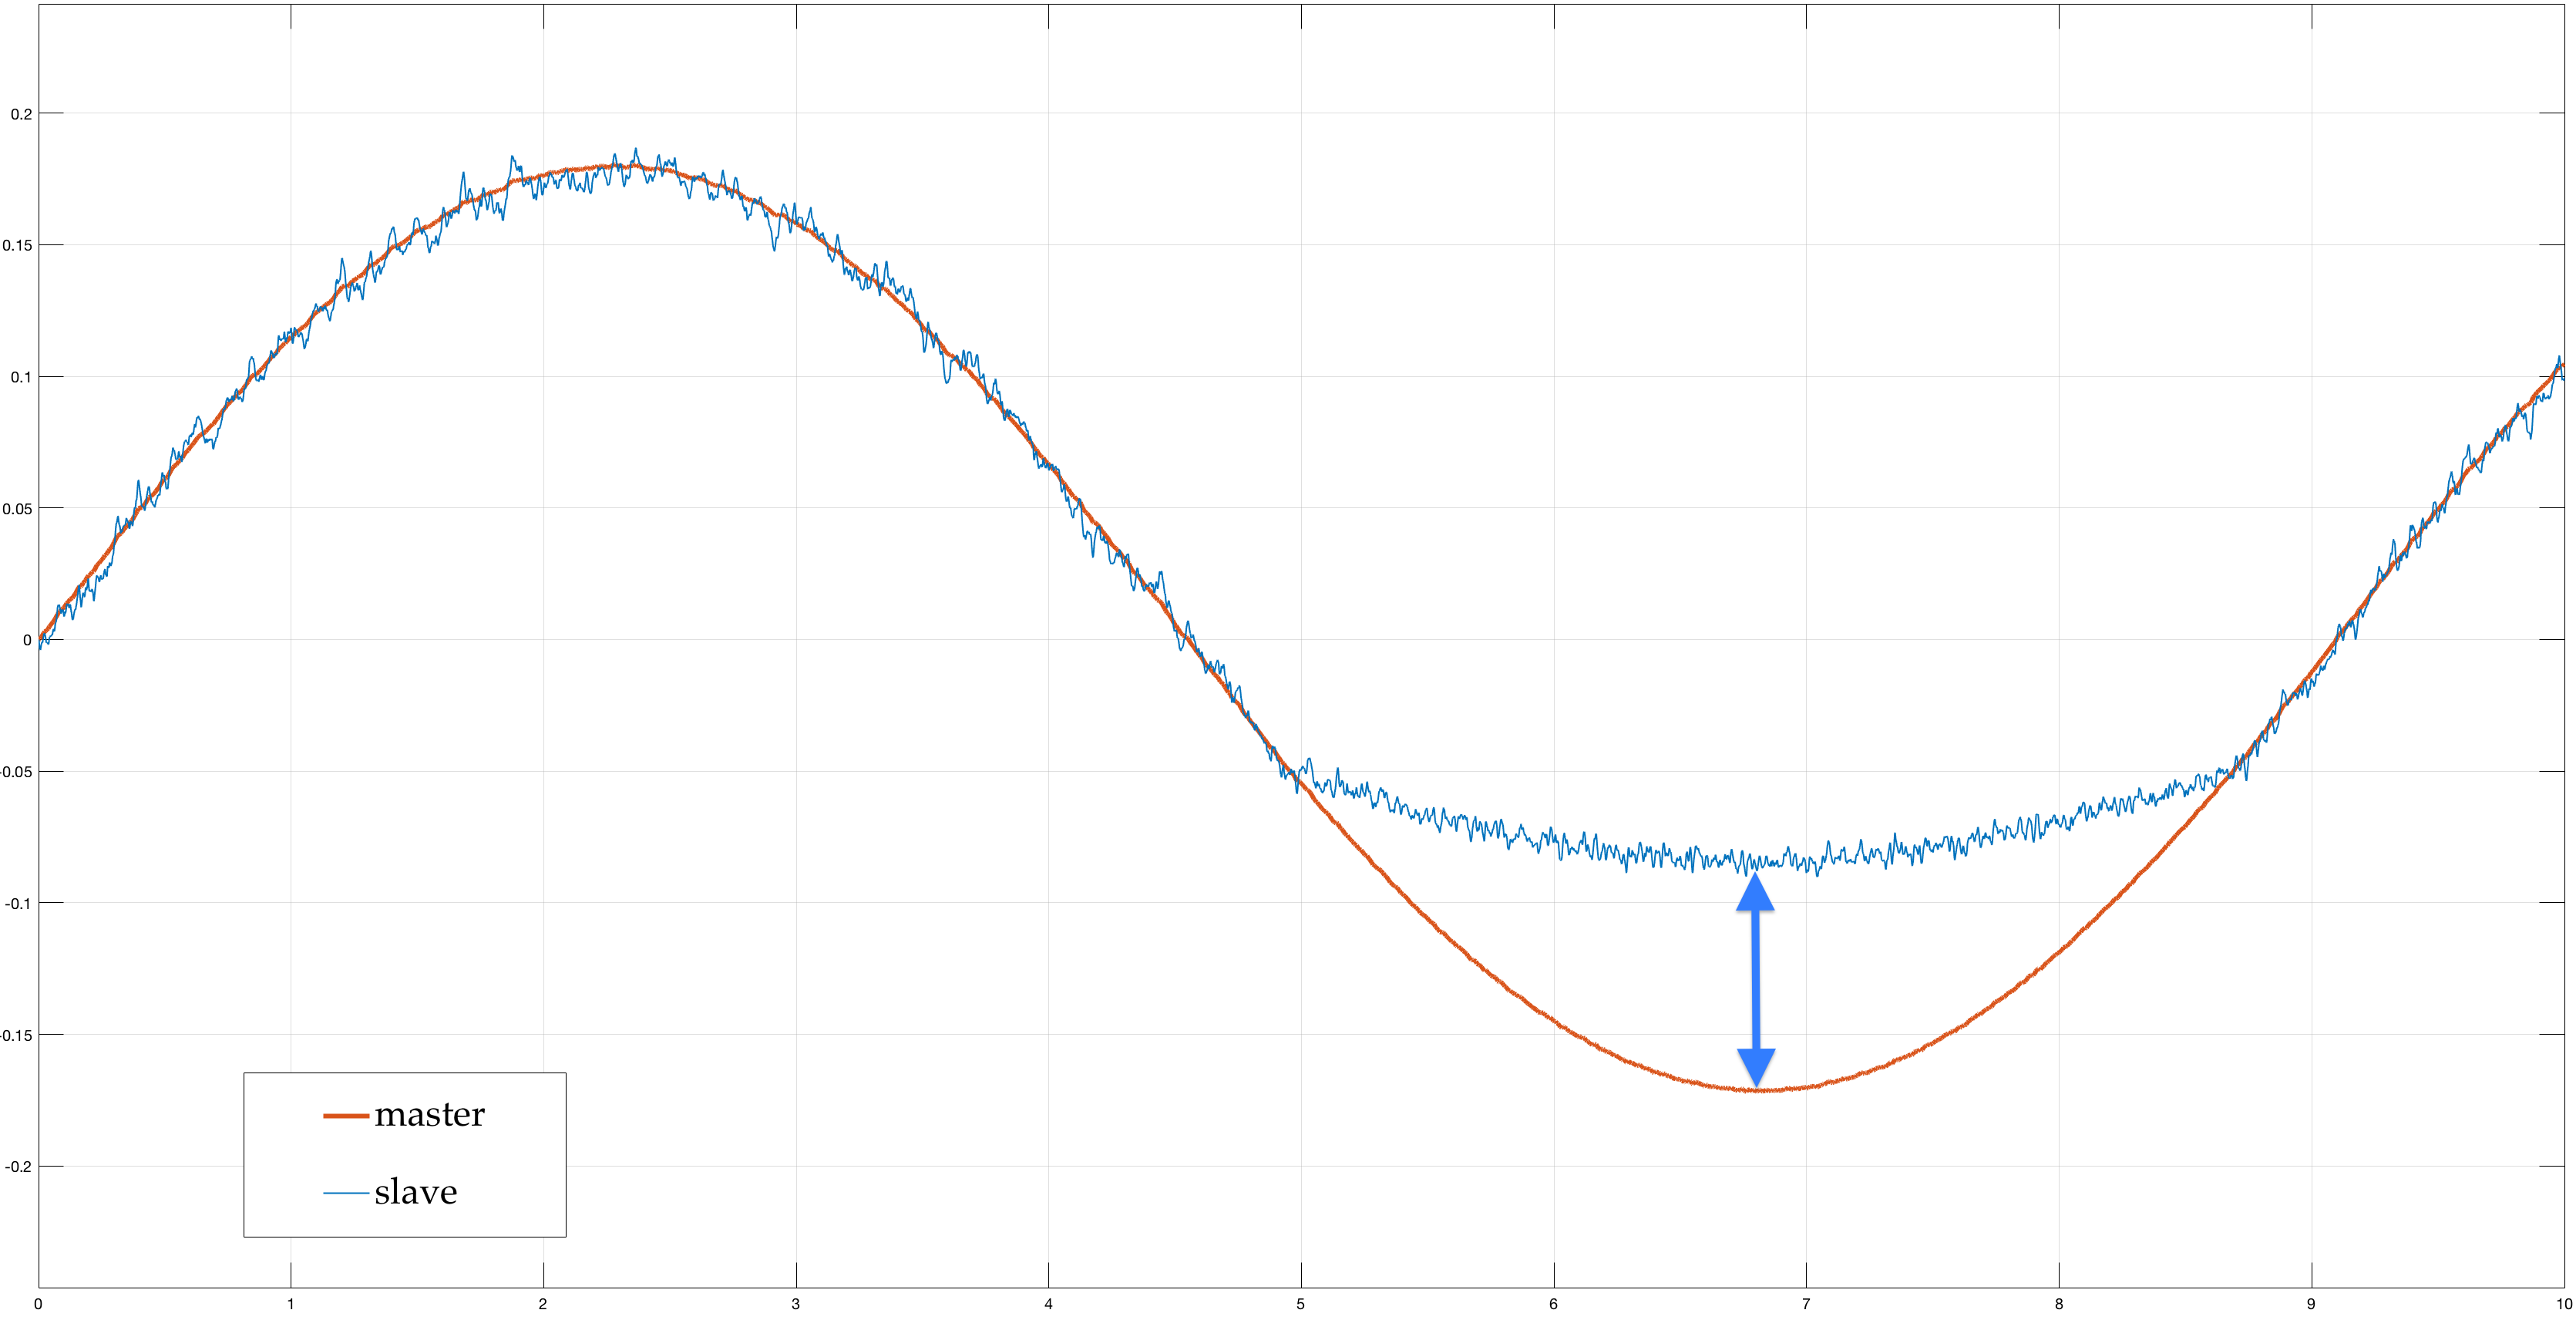
\includegraphics[width=1\linewidth]{Images/setPointContactReacPosArrow}
% 	\caption{bodo}
% 	\label{fig:ContactSetPos}
% \end{figure}

% \begin{figure}[h]
% 	\centering
% 	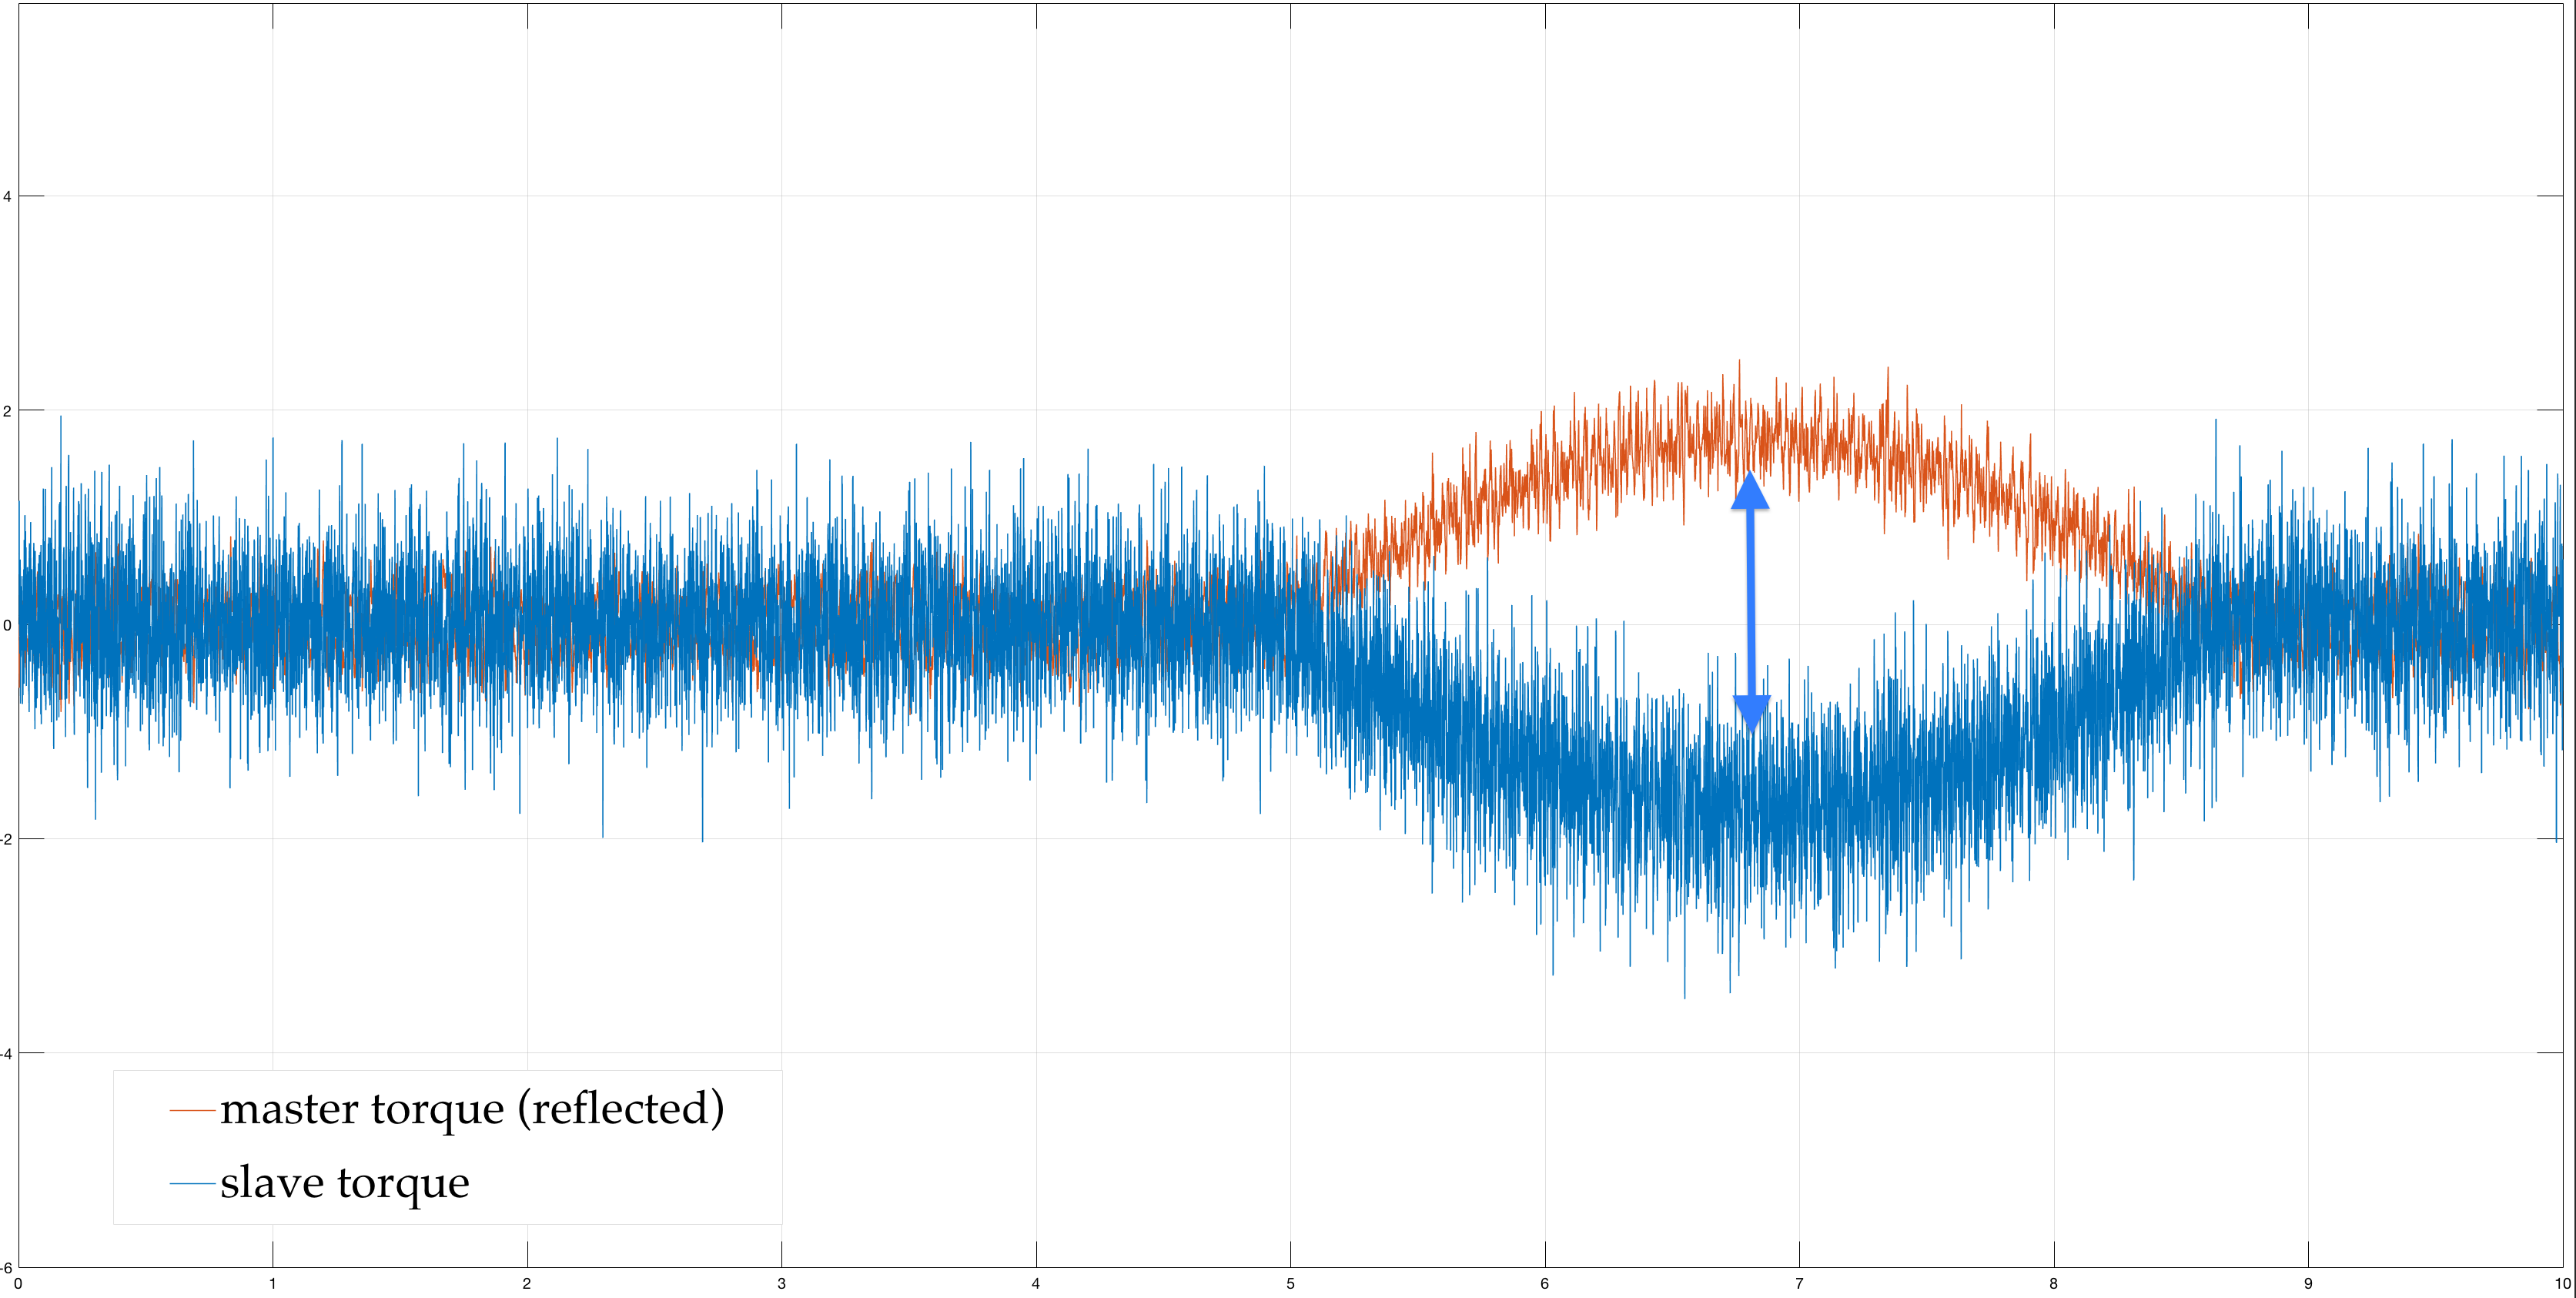
\includegraphics[width=1\linewidth]{Images/setPointContactReacTorArrow}
% 	\caption{bodo}
% 	\label{fig:ContactSetTor}
% \end{figure}

% \begin{figure}[h]
% 	\centering
% 	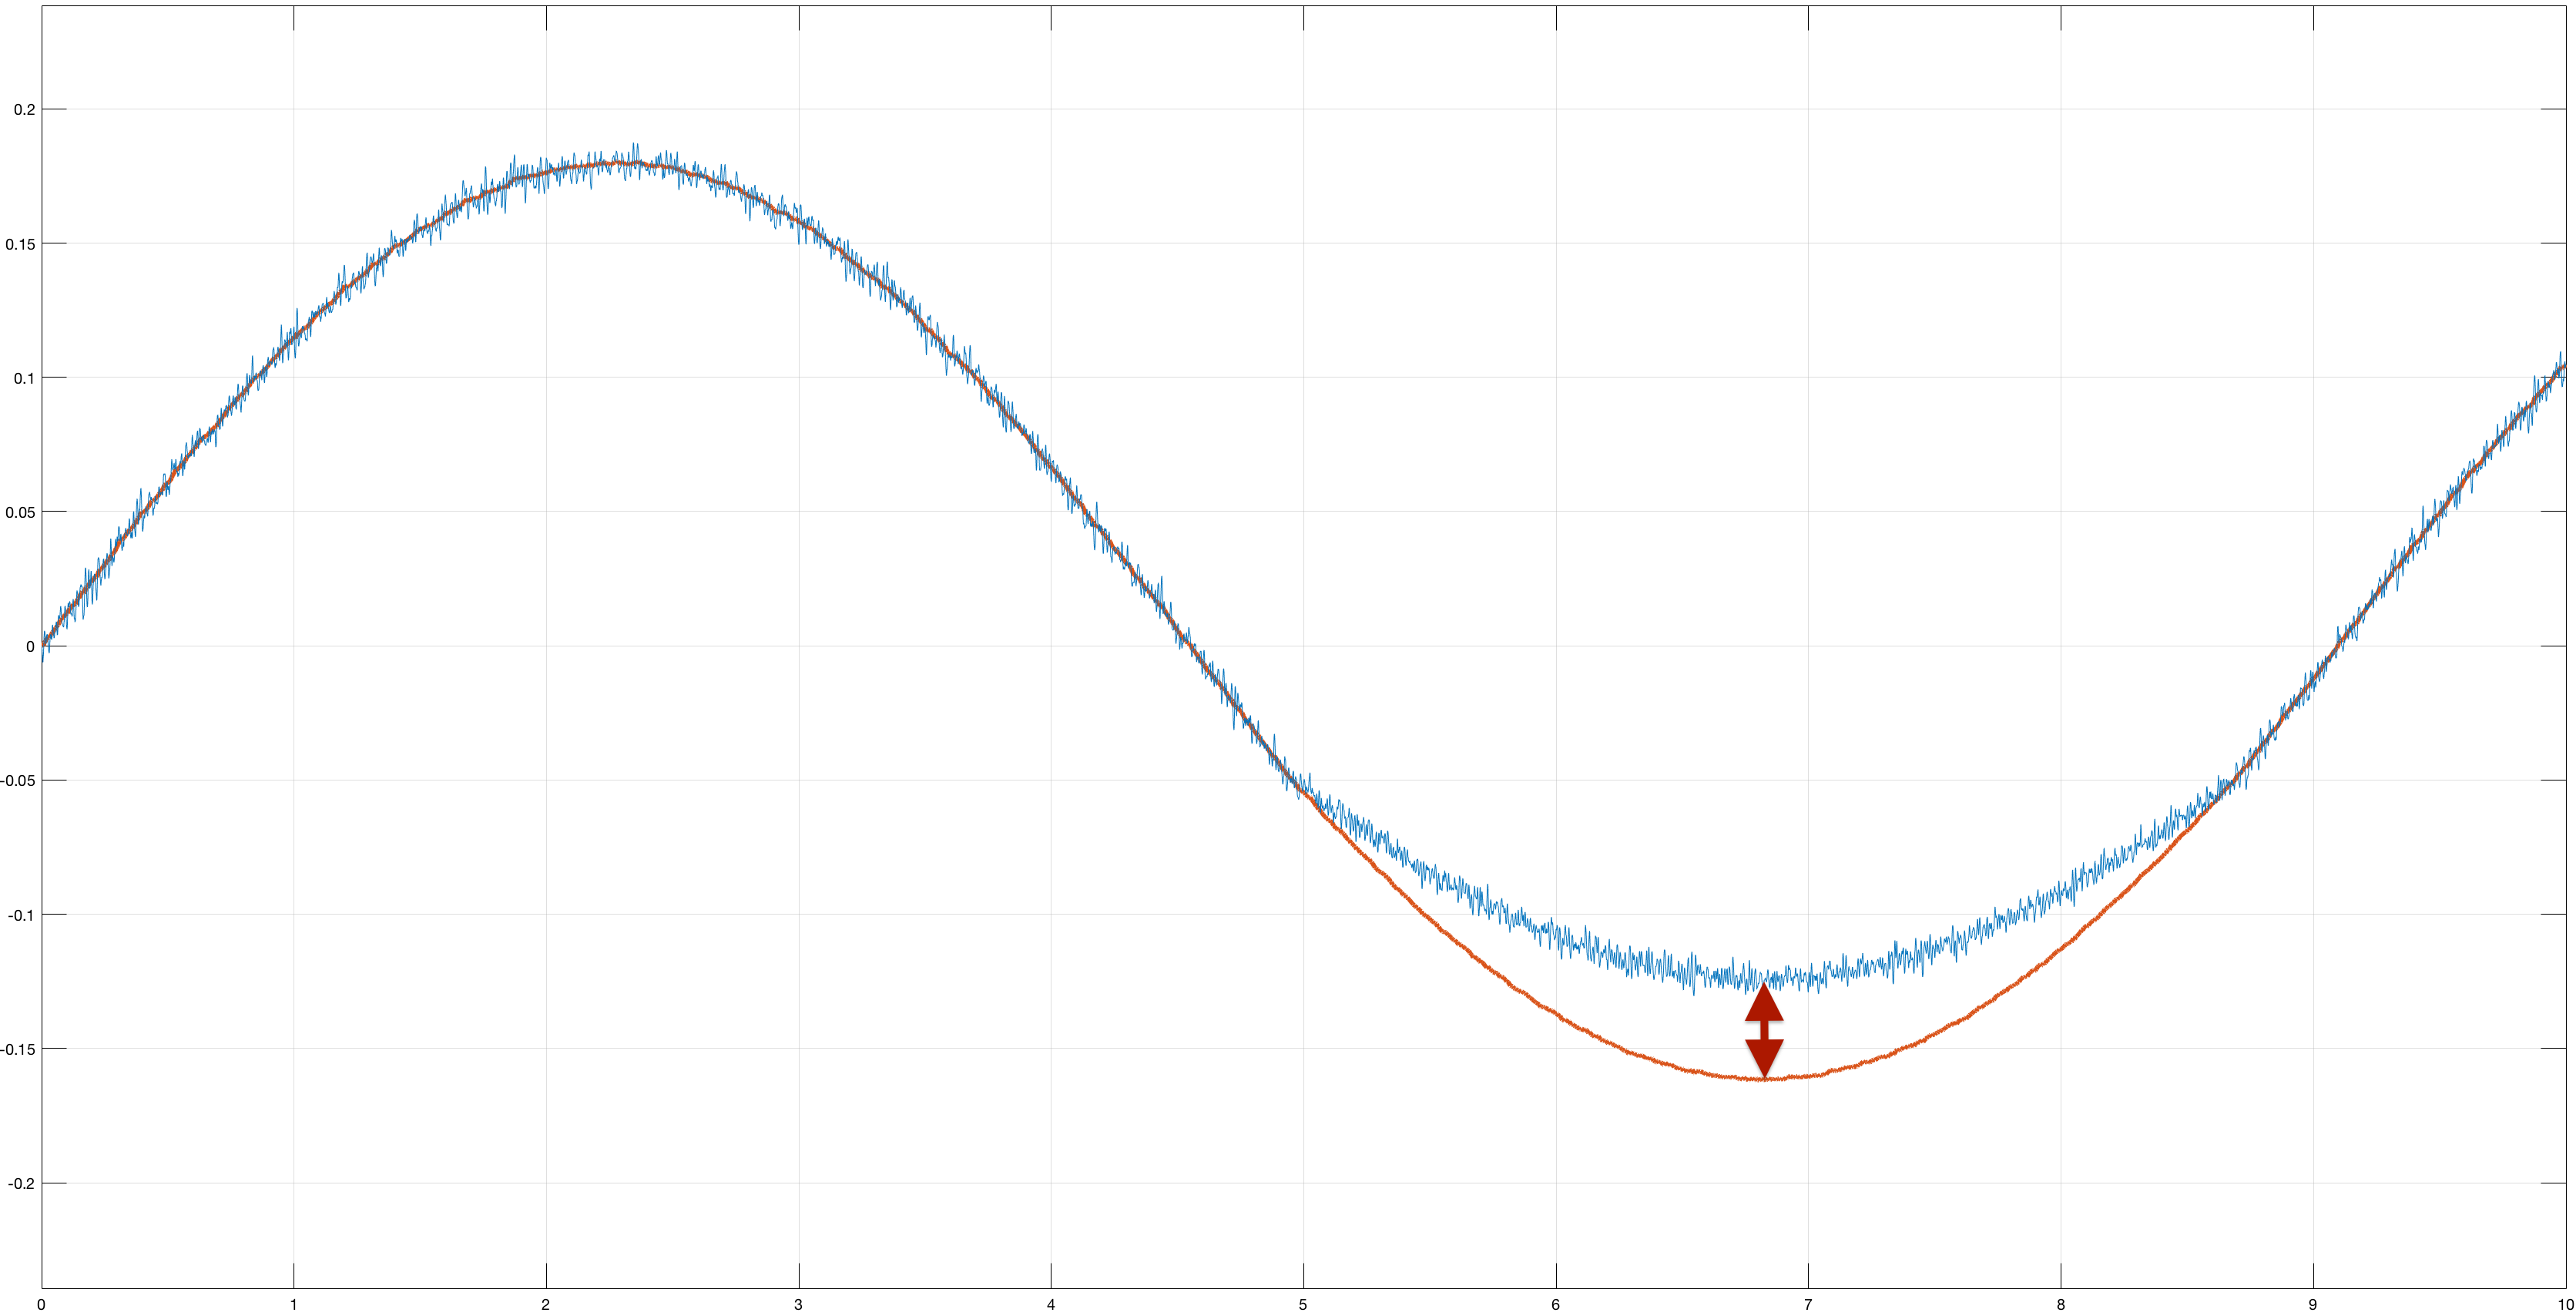
\includegraphics[width=1\linewidth]{Images/rigidContactReacPosArrow}
% 	\caption{bodo}
% 	\label{fig:ContactRigPos}
% \end{figure}

% \begin{figure}[h]
% 	\centering
% 	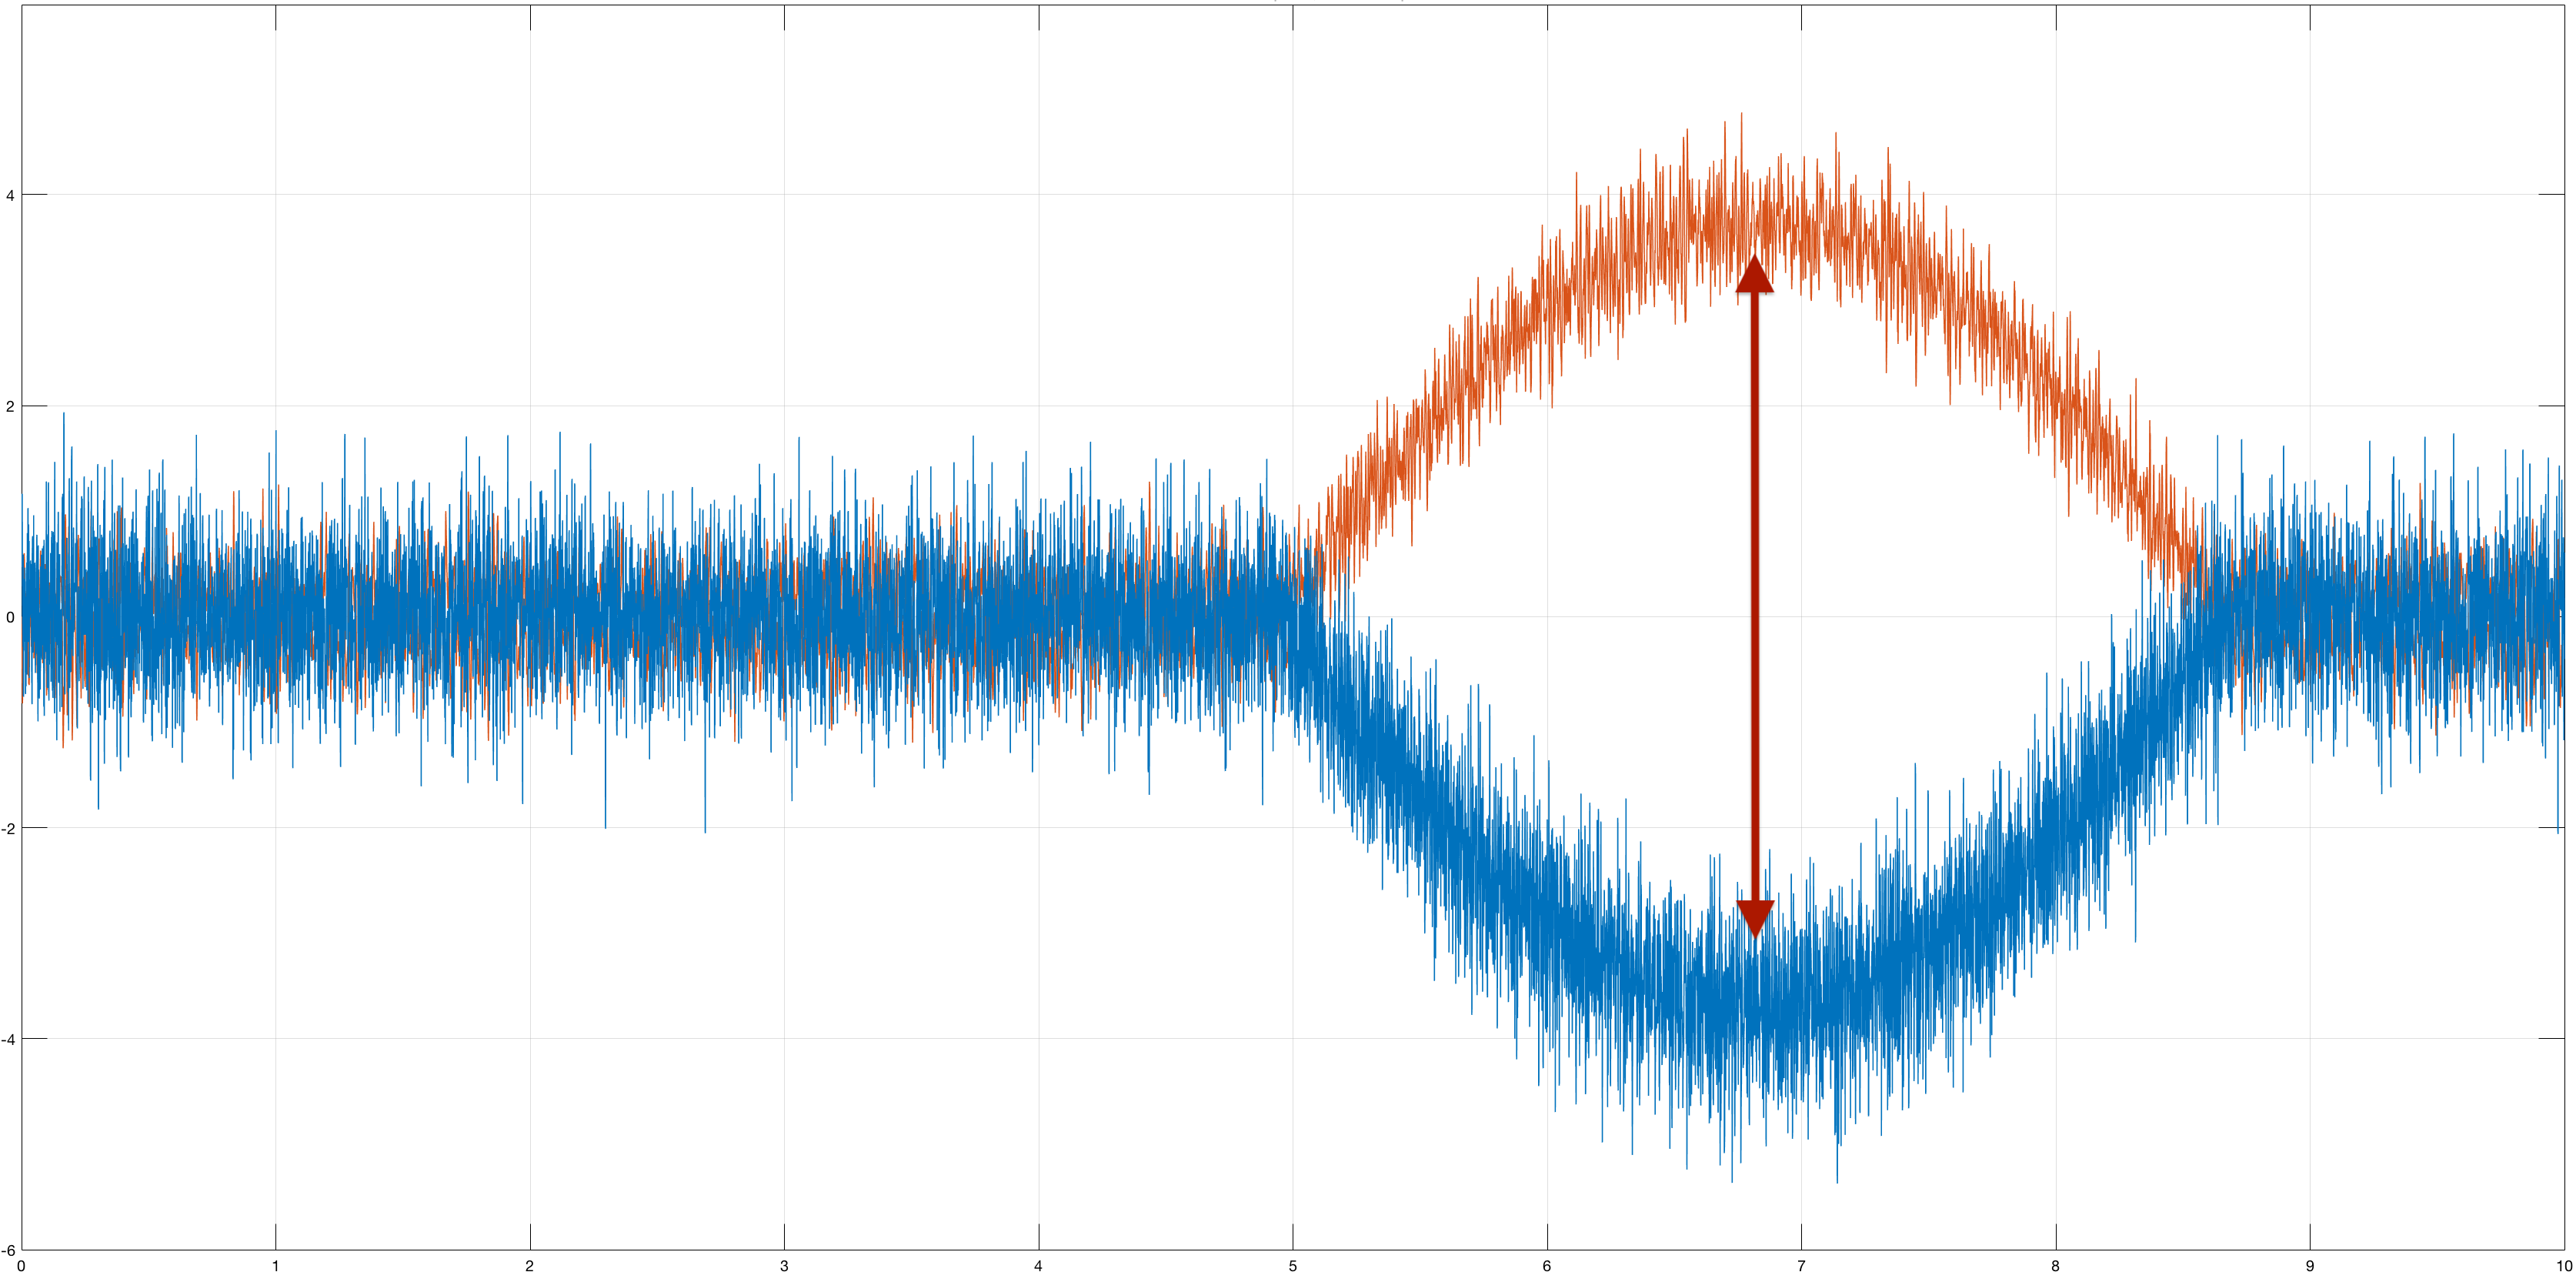
\includegraphics[width=1\linewidth]{Images/rigidContactReacTorArrow}
% 	\caption{bodo}
% 	\label{fig:ContactRigTor}
% \end{figure}


\newpage
\section{Conclusions}
% Furthermore, this kind of vibrations ( $\approx 10^3 Htz$ ) are more likely to belong
% to environment noise are
% filtered  out with greater efficency by the proposed virtual parameter sets than
% in the rigid coupling behaviour.




% as depicited by fig

